%%================================================
%% Filename: main.tex
%% Encoding: UTF-8
%% Created: 2017-05-20 
%%================================================
\documentclass[bachelor]{zzuthesis}
% \documentclass[%
%   bachelor|master|doctor, % mandatory option
%   openany|openright]{zzuthesis}
% 自定义宏包
\usepackage{docutils}

% 图形文件路径
\graphicspath{{figures/}}

\begin{document}

%%%%%%%%%%%%%%%%%%%%%%%%%%%%%%%%%%%%%%%%%%%%%%%%%%
%% 前言
%%%%%%%%%%%%%%%%%%%%%%%%%%%%%%%%%%%%%%%%%%%%%%%%%%
\frontmatter

%%================================================
%% Filename: cover.tex
%% Encoding: UTF-8
%% Author: Yuan Xiaoshuai - yxshuai@gmail.com
%% Created: 2012-01-14 13:44
%% Last modified: 2016-08-28 21:09
%%================================================
% 研究生论文:学校代码、学号或申请号、密级
\schoolcode{10459}
\id{208010102893000753}
\secretlevel{}

% 论文题目
\ctitle{郑州大学学位论文 \LaTeX\ 模板使用示例}

% 研究生论文:
% 培养院系、学科门类、专业名称、专业学位名称(仅限于专业博士、硕士学位论文)、
% 导师姓名、完成时间
% 本科论文:
% 指导老师、职称、学生姓名、学号、专业、院(系)、完成时间
\cdepartment{物理工程学院}
\csubject{工\hspace{2em}学}
\cmajor{电子科学与技术}
\cauthor{赵钱孙} 
\csupervisor{吴郑王}
\protitle{教授}%
\stuno{201322302XX}%本科论文需要学号
% 时间自动生成
% \cdate{\CJKdigits{\the\year}年\CJKnumber{\the\month}月}
% \cdate{2012年6月}

% 研究生论文:英文封面
\etitle{An Introduction to \LaTeX{} Thesis Template of Zhengzhou University} 
\emajor{Materials Science and Engineering} 
\edepartment{School of Materials Science and Engineering}
\eauthor{Zhao Qiansun} 
\esupervisor{Prof. Wu Zhengwang} 
% \edate{December, 2005}%英文日期自动生成
%封面
\makecover

%%================================================
%% Filename: abstract.tex
%% Encoding: UTF-8
%% Author: Yuan Xiaoshuai - yxshuai@gmail.com
%% Created: 2012-04-24 00:21
%% Last modified: 2016-08-28 21:05
%%================================================
\begin{cabstract}

论文的摘要是对论文研究内容和成果的高度概括。摘要应对论文所研究的问题及其研究目
的进行描述,对研究方法和过程进行简单介绍,对研究成果和所得结论进行概括。摘要应
具有独立性和自创性,其内容应包含与论文全文同等量的主要信息。

论文摘要的书写应力求精确、简明。硕士学位论文建议1000字以内,博士学位论文建议
2000字以内。部分学生用外文撰写学位论文时,博士学位论文的摘要应不少于5000字符,
硕士应不少于2500字符。切忌写成对论文书写内容进行提要的形式,尤其要避免“第1章……
;第2章……;……”这种或类似的陈述方式。摘要中不可出现图片、图表、表格或其他插图材
料。

关键词是为了便于做文献索引和检索工作而从论文中选取出来用以表示全文主题内容信息
的单词或术语。关键词应体现论文特色,具有语义性,在论文中有明确的出处,并应尽量
采用《汉语主题词表》或各专业主题词表提供的规范词。在摘要内容下方另起一行标明,
一般3~8个,之间用空格分开。为便于国际交流,应标注与中文对应的英文关键词。

\zzuthesis{}(郑州大学学位论文模板)提供郑州大学本科毕业设计(论文)和研究生学位
论文的模板,其代码来源于清华大学学位论文模板(\textsc{ThuThesis}),并根据《郑州
大学材料科学与工程学院本科毕业设计(论文)基本规范》和《郑州大学学位论文写作规范
格式》的规范要求进行了修改,目前该模板已基本符合学校学院的相关要求。本文介绍该
模板的使用方法,并给出相关示例。

本文的创新点主要有:

  \begin{itemize}
    \item 用例子来解释模板的使用方法;
    \item 用废话来填充无关紧要的部分;
    \item 一边学习摸索一边编写新代码。
  \end{itemize}

\textsf{模板作者声明}:关键词分隔符用半角逗号,模板会自动处理替换为《规范》中
规定的分隔符,英文关键词同理。该分隔符在 \verb|zzuthesis.cfg| 中定义。

\ckeywords{\TeX{}/\LaTeX{}, \XeLaTeX{}与中文处理, 科技排版, 郑州大学, 学位论文
模板, 关于摘要}

\end{cabstract}

\begin{eabstract} 

An abstract of a dissertation is a summary and extraction of research work and
contributions. Included in an abstract should be description of research topic
and research objective, brief introduction to methodology and research
process, and summarization of conclusion and contributions of the research. An
abstract should be characterized by independence and clarity and carry
identical information with the dissertation. It should be such that the
general idea and major contributions of the dissertation are conveyed without
reading the dissertation. 

An abstract should be concise and to the point. It is recommended that the
abstract of master thesis be less than 1000 characters, and the doctor
dissertation less than 2000 characters accordingly. For students who write
their thesis in foreign languages, the abstract should be no more than 2500 \&
5000 words respectively. It is a misunderstanding to make an abstract an
outline of the dissertation and words ``the first chapter'', ``the second
chapter'' and the like should be avoided in the abstract. No pictures, charts,
tables or illustrations are allowed in the abstract.

Key words are terms used in a dissertation for indexing, reflecting core
information of the dissertation. An abstract may contain 3$\sim$8 key words,
with comma used in between to separate one another. In order to facilitate
international exchanges, Enlish keywords should be marked on the corresponding
keywords in Chinese.

\ekeywords{\TeX/\LaTeX, \XeLaTeX\&Chinese, Scientific typesetting system,
Academic thesis template, Zhengzhou University, About keywords}

\end{eabstract}
%摘要

\tableofcontents%目录

\listoffigures%插图清单,本科论文重新定义为\relax
\listoftables%表格清单,本科论文重新定义为\relax

\makeatletter%符号对照表
  \ifzzu@bachelor\else%%================================================
%% Filename: denotation.tex
%% Encoding: UTF-8
%% Author: Yuan Xiaoshuai - yxshuai@gmail.com
%% Created: 2012-01-14 13:44
%% Last modified: 2016-08-28 21:09
%%================================================
\begin{denotation}

\item[HPC] 高性能计算 (High Performance Computing)
\item[cluster] 集群
\item[Itanium] 安腾
\item[SMP] 对称多处理
\item[API] 应用程序编程接口
\item[PI]	聚酰亚胺
\item[MPI]	聚酰亚胺模型化合物,N-苯基邻苯酰亚胺
\item[PBI]	聚苯并咪唑
\item[MPBI]	聚苯并咪唑模型化合物,N-苯基苯并咪唑
\item[PY]	聚吡咙
\item[PMDA-BDA]	均苯四酸二酐与联苯四胺合成的聚吡咙薄膜
\item[$\Delta G$]  	活化自由能~(Activation Free Energy)
\item [$\chi$] 传输系数~(Transmission Coefficient)
\item[$E$] 能量
\item[$m$] 质量
\item[$c$] 光速
\item[$P$] 概率
\item[$T$] 时间
\item[$v$] 速度
\item[劝学] 君子曰:学不可以已。青,取之于蓝,而青于蓝;冰,水为之,而寒于水。
木直中绳。(车柔)以为轮,其曲中规。虽有槁暴,不复挺者,(车柔)使之然也。故木
受绳则直, 金就砺则利,君子博学而日参省乎己,则知明而行无过矣。吾尝终日而思矣
,  不如须臾之所学也;吾尝(足齐)而望矣,不如登高之博见也。登高而招,臂非加长
也,  而见者远;  顺风而呼,  声非加疾也,而闻者彰。假舆马者,非利足也,而致千
里;假舟楫者,非能水也,而绝江河,  君子生非异也,善假于物也。积土成山,风雨兴
焉;积水成渊,蛟龙生焉;积善成德,而神明自得,圣心备焉。故不积跬步,无以至千里
;不积小流,无以成江海。骐骥一跃,不能十步;驽马十驾,功在不舍。锲而舍之,朽木
不折;  锲而不舍,金石可镂。蚓无爪牙之利,筋骨之强,上食埃土,下饮黄泉,用心一
也。蟹六跪而二螯,非蛇鳝之穴无可寄托者,用心躁也。\pozhehao{} 荀况
\end{denotation}
\fi%本科论文不要求
\makeatother

%%%%%%%%%%%%%%%%%%%%%%%%%%%%%%%%%%%%%%%%%%%%%%%%%%
%% 正文
%%%%%%%%%%%%%%%%%%%%%%%%%%%%%%%%%%%%%%%%%%%%%%%%%%
\mainmatter
%%================================================
%% Filename: chap01.tex
%% Encoding: UTF-8
%% Created: 2017-05-220 
%%================================================
\chapter{\TeX/\LaTeX{}系统概述}
\label{cha:overview}

\TeX{}\footnote{\TeX{}的名称是由三个大写的希腊字母ΤЄΧ组成,在希腊语中这个词是“
科学”和“艺术”的意思。为了方便的缘故,一般都写成“TeX”,念做“teck”。}是一个格式
化排版系统,它一问世便以其排版效果的高质量震动整个出版界。尤其是在排版含有大量
数学公式的科技文献方面更显示了它的优越性。\TeX{}还是一个程序源代码公开的免费排
版系统,因此吸引了许多计算机专家及\TeX{}爱好者为之添砖加瓦。

\TeX{}不仅是一个排版程序,而且是一种程序语言。\LaTeX{}\footnote{\LaTeX{}的读法
应为“lay--teck”,念成“lay--tecks”也可以。}就是使用这种语言写成的一个“\TeX{}宏
包”,它扩展了\TeX{}的功能,使我们很方便地进行富于逻辑性的创作而不是专心于字体
、缩进等这些烦人的东西。

\TeX{}是\LaTeX{}的基石,\LaTeX{}建立在\TeX{}之上;各种宏包和类型文件是\LaTeX{}
大厦的装饰材料。\LaTeX{}是特殊版本的\TeX{},并且加进了很多新功能,使得使用者可
以更为方便的利用\TeX{}的强大功能。使用\LaTeX{}基本上不需要使用者自己设计命令和
宏等,因为\LaTeX{}已经替你做好了。因此,即使使用者并不是很了解\TeX{},也可以在
很短的时间内制成高质量的文件。对于排版复杂的数学公式,\LaTeX{}表现的更为出色。

\LaTeX{}与Word是两种不同类型的文本编辑处理系统,各有所长,如果要对文字编辑性能
和使用便捷程度等作综合评比,Word明显优于\LaTeX{},仅“所见即所得”一项,Word就会
赢得绝大多数用户,但要仅限定在学术报告和科技论文方面,评比结果就不同了:

\section*{从头开始}

Word特点就是“所见即所得”,其基本功能初学者很容易掌握,很多Word用户都是无师自通
。但随着篇幅和复杂程度的增加,花费在文稿格式上的精力和时间要明显加大。因为创建
自定义编号、交叉引用、索引和参考文献等就不是“所见即所得”了,得耐着性子反复查阅
Word的在线帮助或借助相关软件帮忙。

对于\LaTeX{}初学者,即就是编排很简单的文章,也要花较多的精力和时间去学习那些枯
燥的命令和语法,特别是排写数学公式,经常出错,多次编译不能通过,使很多初学者望
而却步。可是一旦掌握,不论文稿长短和复杂与否都会熟练迅速地完成,先前学习
\LaTeX{}的精力投入将由此得到回报。

\section*{内容与样式}

当用Word写作时,要花很多精力对页版式、章节样式、字体属性、对齐和行距等文本参数
进行反复选择对比,尤其是长篇文章,经常出现因疏忽而前后文体格式不一致的现象;当
在稿件中插入或删除一章或章节次序调整时,各章节标题、图表和公式等的编号都要用手
工作相应修改,稍有不慎就会出现重号或跳号。你既是作者又是编辑还兼排字工。

使用\LaTeX{}编版,如无特殊要求,只要将文稿的类型(article、report或book等)告
诉\LaTeX{},就可专心致志地写文章了,至于文稿样式的各种细节都由\LaTeX{}统一规划
设置,而且非常周到细致;当修改稿件时,其中的章节、图表和公式等的位置都可任意调
整,无须考虑编号,因为在源文件里就没有编号,文件中的所有编号都是在最后编译时
\LaTeX{}自动统一添加的,所以绝对不会出错。

换句话说,Word把文稿的内容与样式混为一体,而\LaTeX{}将它们分离,作者只需专注于
文稿的内容,而文稿的样式几乎不用过问,\LaTeX{}是你的聪明而忠诚的文字秘书,如有
特殊要求,也可使用命令修改,\LaTeX{}会自动将相关设置更新,无一遗漏。

接受\LaTeX{}稿件的出版社大都有自己的文稿样式模板,主要就是一个类型文件包,简称
类包。如果稿件未被甲出版社采用,在转投乙出版社前,只需将稿件第一句中类包名称由
甲出版社的改为乙出版社的,整篇稿件的样式就随之自动转换过来了。就一句话的事儿,
简单的不能再简单了,然而因为“体制”的原故,Word却根本无法做到这一点。

\section*{数学公式}

Word有个公式编辑器,可以编辑普通数学公式,但使用很不方便,外观效果较差,也不能
自动编号,尤其是很难作为文本的一部分,融入某一行中,大都专起一行。如果碰到复杂
的数学公式,编辑起来就很困难。有些用户只好另外安装可嵌入Word环境的工具软件
Math-Type来弥补这一不足。

\LaTeX{}的特长之一就是数学公式编辑,方法简单直观,“所想即所得”,公式的外观精致
细腻,而且公式越复杂这一优点就越明显。普通单行公式可以像纯文字文本一样插入字里
行间。尽管在默认状态下,就能将数学公式编排的非常精致美观,\LaTeX{}仍然还提供了
很多调节命令,可以对公式的外观作更加细微的调整,使其尽善尽美。

\section*{插图}

Word有个绘图工具,简易直观,但功能有限效果不佳。论文中的复杂图形大都用功能强大
的Visio、Photoshop等绘图软件绘制,然后插入Word。

\LaTeX{}自身也具有简单的绘图功能,如调用各种绘图宏包,可画出非常复杂的图形,缺
点是不直观,命令格式繁琐,不易熟练掌握,名曰画图,实为编程。可同样先使用Visio
绘图,然后粘贴到Adobe Illustrator,对图形的细节作进一步处理后,存储为PDF或EPS
格式,最后用插图命令调入\LaTeX{}源文件即可,其效果更为精致。

\section*{创建参考文献}

Word目前还不具备管理参考文献的功能,用户一般都是采用Reference Manager或是
NoteExpress等外部工具软件来解决这一问题。

创建参考文献可是\LaTeX{}的强项。\LaTeX{}自带一个辅助程序\BibTeX{},它可以根据
作者的检索要求,搜索一个或多个文献数据库,然后自动为文稿创建所需的参考文献条目
列表。如果编写其它文件用到相同的参考文献时可直接引用这个数据库。参考文献的样式
和排序方式都可以自行设定。

很多著名的科技刊物出版社、学术组织和TUG网站等都提供相关的\BibTeX{}文献数据库文
件,可免费下载。

\section*{显示与输出}

在文本对齐、字体变换、拼写检查、单词间距控制、自动断词和自动换行等纯文字处理功
能方面,Word经多次升级后已与\LaTeX{}相差无几,但是排版效果却有所不同。以Times
字体为例,在Word中“Ta”和“PA”两个字母的间距有些松散。\LaTeX{}将各种拼写组合时的
字母间距进一步优化调整,松紧得当,使整个文本的排版效果更加工整匀称。

在换行时,\LaTeX{}不仅可以根据音节自动断词,也可以按照作者的要求进行设定断词,
一个单词可以设定多种断词方式,特别适用于科技论文中反复出现的专业词汇或缩略写,
这既能保持单词间距均匀,又不易产生误解。

在科技著作手稿中经常可以看到某些论述附有说明、出处或考证;或者某些段落划上黑杠
以示删除;或在边空里写有准备补充的文字。在\LaTeX{}源文件中使用注释标记可以将上
述这些内容完整地保留下来,以备后用,而在编译后的PDF文件中还看不到这些内容。科
研论文要经过反复推敲,多次修改,注释功能非常实用。“所见即所得”的Word,当然没有
这个功能,它删除的内容就甭想再找回来了。

一篇论文,Word新手与牛人的排版美观程度差别很大,“所见即所得”成了一大缺点,因为
Word本身不能帮助作者美化作品,自己排成什么样就什么样,即:“所得仅所见”,就像在
白纸上作画,全凭个人的悟性与灵感。而\LaTeX{}初学与专家的排版外观差别很小,仅是
快慢不同,都能达到专业出版水平,这就是\LaTeX{}的一大优点,只要想法一致就能得到
相同的结果,也就是“所想即所得”。

目前PDF格式已成为全世界各种组织机构用来进行更加安全可靠的电子文件分发和交换的
出版规范,科技论文大都使用PDF格式。\LaTeX{}可以直接输出PDF、PS或DVI格式文件;
而Word输出的是DOC格式文件,还须将DOC转换为PDF;另外,图形中的数学公式或文本中
数学式的上下标,在转换后常出现位置偏移字形变大等问题。

\section*{可扩充性}

用户可以像搭积木那样对\LaTeX{}进行功能扩充或添加新的功能。例如,加载一个CJK宏
包,就可以处理中文,调用eucal宏包可将数学公式中的字符改为欧拉书写体;如果对某
个宏包效果不太满意,完全可以打开来修改,甚至照葫芦画瓢自己写一个。这些可附加的
宏包文件绝大多数都可从CTAN等网站无偿下载。

因为设计的超前性,\TeX{}/\LaTeX{}程序系统几十年来没有什么改动,而且由于它的可
扩充性,\LaTeX{}将永葆其先进性,也就是说,学习和使用\LaTeX{}永远不会过时。例如
,通过调用相关扩展宏包,\LaTeX{}立刻就具备了排版高质量高专业水准象棋谱、五线谱
或化学分子式的能力。对于\LaTeX{}这种机动灵活、简便免费的可扩充性能,Word只能望
尘。

\section*{稳定性和安全性}

一篇科技论文少则几十页,多则上百页,其中含有许多图形和公式(Word将公式处理为图
形),正是由于Word“所见即所得”,论文中的图形都要完整地插入页面。随着文件的篇幅
增大图形数量增多,处理速度明显减慢。编写一篇论文要无数次地打开、保存和关闭,往
往要长时间等待甚至死机或文稿无法打开,所以Word经常出现“文件恢复”提示信息,但其
中的图形很有可能丢失,取而代之的是一个小红叉。如果将文件分解为多个子文件,可以
缓解这一问题,但又会出现难以自动创建目录、索引和参考文献等新问题;若章节、图表
和公式需要在子文件之间调换调整,那编号就全乱套了。

\LaTeX{}是纯文本文件,所有图形都是在最后编译时调入。同一篇文章,其\LaTeX{}源文
件只有Word文件尺寸的几十分之一。所以,\LaTeX{}源文件的长短,不会对文件存取和编
辑过程产生明显影响。\LaTeX{}也允许采用多个子文件,章节和图表可随意增删,
\LaTeX{}是在最后编译时才将所有子文件汇总排序,生成统一的文件页码、标题序号、图
表和公式编号以及各种目录。

Word从问世到现在不断地更新版本,并经常要求下载补丁程序,防止病毒攻击。\LaTeX{}
及其前身\TeX{},近二十年来,没有发现系统漏洞,即使有,造成源文件损坏的风险也是
微乎其微;迄今也未发现任何宏包含有病毒。

\section*{版本兼容性}

Word十几年里已有多种版本,只能向下兼容,旧文件在新版本中打开,经常出现字形和文
本位置变动等问题。

二十年来\LaTeX{}也有几种版本,但可相互兼容,旧文件在新版本中打开,文本不会有丝
毫的变形,而且还可以继续追加新的功能,如这几年很流行的超文本链接和PDF书签等。

\section*{通用性}

随着计算机软硬件性能的提高,在PC机上使用Unix/Linux、MacOS或其他操作系统的用户
越来越多。由于\LaTeX{}系统的程序源代码是公开的,因此人们开发了用于各种操作系统
的版本,而且\LaTeX{}源文件全部采用国际通行的ASCII字符,所以\LaTeX{}及其源文件
可以毫无阻碍地跨平台、跨系统使用和传播。

而Word只能在Windows操作系统上运行。

高德纳教授曾说过:TeX排版系统追求的首要目标就是高品质,文件的排印效果不只是很
好,而是要最好。\LaTeX{}就是专门为排版高质量科技论文而设计的软件,当然在这方面
的性能就非常突出。在很多\LaTeX{}爱好者看来,\LaTeX{}不仅是一种文字编辑排版工具
,它更是一门艺术,给人以美的享受。然而,追求完美是要付出一定代价的,是否值得,
那得您说了算!


%%================================================
%% Filename: chap02.tex
%% Encoding: UTF-8
%% Author: Yuan Xiaoshuai - yxshuai@gmail.com
%% Created: 2012-04-27 19:37
%% Last modified: 2016-08-29 21:07
%%================================================
\chapter{模板简介及安装}
\label{cha:introduction}

\zzuthesis(\textbf{Z}heng\textbf{z}hou \textbf{U}niversity \textbf{Thesis})以
标准book类文档为基础,根据清华大学学位论文模板修改而来。本科毕业设计(论文)
和研究生学位论文(含硕士和博士)分别根据《郑州大学材料科学与工程学院本科毕业
设计(论文)基本规范》和《郑州大学学位论文写作规范格式》的规范要求定制,目前
该模板已基本符合相关《规范》的要求。除格式方面的修改外,还参考其它论文模板,
尽可能简化了代码,更有利于初学者使用。

\textsf{模板作者声明:}该模板非学校官方模板,尽管模板基本满足《规范》要求,并
参考2011年通过审核的学位论文进行调整,但难免还存在不足之处,欢迎大家反馈。

% \section{本科毕业设计论文内容要求}
% \label{sec:bachelor}
% 
% 根据《郑州大学材料科学与工程学院本科毕业设计(论文)基本规范》的要求,本科
% 毕业设计(论文)的装订如下:封面(格式版式固定,只替换文字),中文摘要,英
% 文摘要,目录,1. 前沿(概述),2. 实验过程(方法),3. 实验结果与讨论,4.
% 结论,5 . 参考文献,6. 表格附件(毕业设计(论文)任务书、郑州大学毕业论文开
% 题报告表、毕业设计(论文)计划进程表、郑州大学毕业设计中期检查表、毕业论文
% (论文)成绩评定表),7. 外文翻译,8. 外文原文,9. 致谢。
% 
% \section{研究生论文内容要求} \label{sec:graduates}
% 
% 根据二〇〇九年十月郑州大学学位办公室编制的《郑州大学博士、硕士学位论文写作
% 规范》的要求,学位论文一般由十五部分组成,依次为:1. 封面;2.英文封面;3.
% 学位论文原创性声明;4. 学位论文使用授权声明;5. 摘要;6. Abstract;7. 目录
% ;8.图和附表清单;\footnote{模板将图和附表清单分为插图清单和附表清单两个部
% 分}9.符号说明;10. 正文;11.注释;12. 参考文献;13. 致谢;14. 附录;15. 个
% 人简历、在学期间发表的学术论文及研究成果。
  
\section{模板系统需求}
\label{sec:requirements}

\TeXLive{}为多种基于Unix的平台提供了可执行文件\footnote{\TeXLive{}的安装参见:
\url{http://tug.org/texlive/acquire.html}。},包括GNU/Linux、Mac OS X、和
Cygwin,并支持Windows XP及后续版本。理论上该模板应该在常见的系统平台上都可以正
常运行,但仅在以下系统平台下进行了测试:
\begin{enumerate}
\item Fedora 16 + \TeXLive{} 2011 + Jabref 2.8
\item Windows XP + \TeXLive{} 2011 + Jabref 2.8
\end{enumerate}

由于模版文件中用到的部分命令在最新的发行版中有所更改,故在 2016 年 8 月 28 日
对模版进行修改,并在以下平台测试通过:

\begin{itemize}
\item CentOS 7.2.1511 + \TeXLive{} 2015
\end{itemize}

\section{模板的组成部分}

下表列出了 \zzuthesis{} 的主要文件及其功能介绍:
\begin{center}
\tablefirsthead{%
\hline
{\hei 文件(夹)} & {\hei 功能描述}\\\hline\hline}
\tablehead{\hline
{\hei 文件(夹)} & {\hei 功能描述}\\\hline\hline}
% \endhead
\tabletail{\hline}
% \endfoot
  \begin{mpsupertabular}{l|p{8cm}}
zzuthesis.cls & 模板类文件\\
zzuthesis.cfg & 模板配置文件\\
zzubib.bst & 参考文献样式文件\\\hline
docutils.sty & 模板示例文档用到的宏包及定义\footnote{使用该模板时可根据需要加
入其它自定义宏包及定义。}\\ 
main.tex & 示例文档主文件\\
spine.tex & 书脊示例文档\\
a3cover.tex & A3封面示例文档\\
ref/ & 示例文档参考文献目录\\
data/ & 示例文档章节具体内容\\
figures/ & 示例文档图片路径\\
fonts/ & 模版中用到的字体文件\\\hline
Makefile & Linux 自动编译工具\\
msmake.cmd & Windows 批处理工具\\
  \end{mpsupertabular}
\end{center}

该模板可以通过以下途径获取:
\begin{itemize}
\item 浏览器下载:
\href{https://codeload.github.com/tuxify/zzuthesis/zip/master}{Github Download Zip}
\item Git 命令:
\texttt{git clone https://github.com/tuxify/zzuthesis.git}
\end{itemize}

\section{准备工作}

模板中调用的宏包有:
\begin{center}
\begin{minipage}{1.0\linewidth}\centering
\begin{tabular}{*{7}{l}}\hline
calc & titletoc & amsmath & amssymb & amsthm & \\% txfonts 
geometry & tabularx & multirow & longtable & booktabs & subfig\footnote{版本要求:$\geq$2005/06/28 ver: 1.3} \\
graphicx & indentfirst\footnote{2016/8/28修改后首段不缩进,添加该宏包后解决} & paralist & xeCJK & natbib & hyperref \\
hypernat & & & & &\\\hline
\end{tabular}
\end{minipage}
\end{center}

这些包在常见的 \TeX{} 系统中都有,如果没有请到 \url{www.ctan.org} 下载。

模板中用到的字体有:
\begin{itemize}
\item 中文字体:Adobe Song Std、Adobe Heiti Std、Adobe Kaiti Std、Adobe Fangsong
Std;STXingkai\footnote{研究生论文封面需要用到该种字体。}、STZhongsong。
\item 英文字体:Times New Roman、Arial、Courier New。
\end{itemize}

模板使用\XeTeX{}避免了繁琐的字体配置,并通过xeCJK来控制中文字体。故只需把上述
字体放入系统文件夹即可。

\section{示例文档的生成}

示例文档的生成需要多次运行\XeLaTeX{},直到不再出现警告为止,详细过程如下:
\begin{code}
1. 发现文档的引用关系,文件后缀 .tex 可以省略
$ xelatex main
2. 编译参考文件源文件,生成 bbl 文件
$ bibtex main
3. 解决引用
$ xelatex main
4. 生成完整的 pdf 文件
$ xelatex main
\end{code}

由于一般情况下的使用方法每次需要输入数次命令,比较麻烦,故模板提供了一些自动
处理的文件。

Linux平台可以使用 \emph{Makefile} 文件:
\begin{code}
$ make thesis    # 生成示例文档
$ make a3cover   # 生成A3封面
$ make clean     # 清除临时文件
\end{code}

对于Windows平台,则提供了一个批处理脚本 \emph{msmake.cmd}\/:
\begin{code}
your_path $ msmake thesis  # 生成示例文档
your_path $ msmake a3cover # 生成A3封面
your_path $ msmake clean   # 清除临时文件
\end{code}

%%================================================
%% Filename: chap03.tex
%% Encoding: UTF-8
%% Created: 2017-05-20 
%%================================================
\chapter{关于该模板的使用}
\label{cha:usage}

模板核心文件只有三个:\emph{zzuthesis.cls},\emph{zzuthesis.cfg} 和
\emph{zzubib.bst},其中定义的命
令分为两类:一是格式控制,二是内容替换。格式控制如字体、字号、字距和行距。内容
替换如姓名、院系、专业、致谢等等。模板自带的示例文档里面基本涵盖了论文写作用到
的所有命令及其使用方法,只需要用自己的内容进行相应替换就可以。本章将会对模板中
的命令及其使用作一简要介绍。

\section{\zzuthesis{} 示例文件}

下面的例子描述了模板中章节的组织形式,来自于示例文档,具体内容可以参考模板附
带的 \emph{main.tex} 和 \emph{data}\//。
\begin{code}
\documentclass[bachelor]{zzuthesis}
% \documentclass[%
%   bachelor|master|doctor, % mandatory option
%   openany|openright]{zzuthesis}

\usepackage{docutils}%模板文档用到的宏包及定义

\graphicspath{{figures/}}
\end{code}
\begin{code}
\begin{document}
\frontmatter
%%================================================
%% Filename: cover.tex
%% Encoding: UTF-8
%% Author: Yuan Xiaoshuai - yxshuai@gmail.com
%% Created: 2012-01-14 13:44
%% Last modified: 2016-08-28 21:09
%%================================================
% 研究生论文:学校代码、学号或申请号、密级
\schoolcode{10459}
\id{208010102893000753}
\secretlevel{}

% 论文题目
\ctitle{郑州大学学位论文 \LaTeX\ 模板使用示例}

% 研究生论文:
% 培养院系、学科门类、专业名称、专业学位名称(仅限于专业博士、硕士学位论文)、
% 导师姓名、完成时间
% 本科论文:
% 指导老师、职称、学生姓名、学号、专业、院(系)、完成时间
\cdepartment{物理工程学院}
\csubject{工\hspace{2em}学}
\cmajor{电子科学与技术}
\cauthor{赵钱孙} 
\csupervisor{吴郑王}
\protitle{教授}%
\stuno{201322302XX}%本科论文需要学号
% 时间自动生成
% \cdate{\CJKdigits{\the\year}年\CJKnumber{\the\month}月}
% \cdate{2012年6月}

% 研究生论文:英文封面
\etitle{An Introduction to \LaTeX{} Thesis Template of Zhengzhou University} 
\emajor{Materials Science and Engineering} 
\edepartment{School of Materials Science and Engineering}
\eauthor{Zhao Qiansun} 
\esupervisor{Prof. Wu Zhengwang} 
% \edate{December, 2005}%英文日期自动生成
%封面
\makecover

%%================================================
%% Filename: abstract.tex
%% Encoding: UTF-8
%% Author: Yuan Xiaoshuai - yxshuai@gmail.com
%% Created: 2012-04-24 00:21
%% Last modified: 2016-08-28 21:05
%%================================================
\begin{cabstract}

论文的摘要是对论文研究内容和成果的高度概括。摘要应对论文所研究的问题及其研究目
的进行描述,对研究方法和过程进行简单介绍,对研究成果和所得结论进行概括。摘要应
具有独立性和自创性,其内容应包含与论文全文同等量的主要信息。

论文摘要的书写应力求精确、简明。硕士学位论文建议1000字以内,博士学位论文建议
2000字以内。部分学生用外文撰写学位论文时,博士学位论文的摘要应不少于5000字符,
硕士应不少于2500字符。切忌写成对论文书写内容进行提要的形式,尤其要避免“第1章……
;第2章……;……”这种或类似的陈述方式。摘要中不可出现图片、图表、表格或其他插图材
料。

关键词是为了便于做文献索引和检索工作而从论文中选取出来用以表示全文主题内容信息
的单词或术语。关键词应体现论文特色,具有语义性,在论文中有明确的出处,并应尽量
采用《汉语主题词表》或各专业主题词表提供的规范词。在摘要内容下方另起一行标明,
一般3~8个,之间用空格分开。为便于国际交流,应标注与中文对应的英文关键词。

\zzuthesis{}(郑州大学学位论文模板)提供郑州大学本科毕业设计(论文)和研究生学位
论文的模板,其代码来源于清华大学学位论文模板(\textsc{ThuThesis}),并根据《郑州
大学材料科学与工程学院本科毕业设计(论文)基本规范》和《郑州大学学位论文写作规范
格式》的规范要求进行了修改,目前该模板已基本符合学校学院的相关要求。本文介绍该
模板的使用方法,并给出相关示例。

本文的创新点主要有:

  \begin{itemize}
    \item 用例子来解释模板的使用方法;
    \item 用废话来填充无关紧要的部分;
    \item 一边学习摸索一边编写新代码。
  \end{itemize}

\textsf{模板作者声明}:关键词分隔符用半角逗号,模板会自动处理替换为《规范》中
规定的分隔符,英文关键词同理。该分隔符在 \verb|zzuthesis.cfg| 中定义。

\ckeywords{\TeX{}/\LaTeX{}, \XeLaTeX{}与中文处理, 科技排版, 郑州大学, 学位论文
模板, 关于摘要}

\end{cabstract}

\begin{eabstract} 

An abstract of a dissertation is a summary and extraction of research work and
contributions. Included in an abstract should be description of research topic
and research objective, brief introduction to methodology and research
process, and summarization of conclusion and contributions of the research. An
abstract should be characterized by independence and clarity and carry
identical information with the dissertation. It should be such that the
general idea and major contributions of the dissertation are conveyed without
reading the dissertation. 

An abstract should be concise and to the point. It is recommended that the
abstract of master thesis be less than 1000 characters, and the doctor
dissertation less than 2000 characters accordingly. For students who write
their thesis in foreign languages, the abstract should be no more than 2500 \&
5000 words respectively. It is a misunderstanding to make an abstract an
outline of the dissertation and words ``the first chapter'', ``the second
chapter'' and the like should be avoided in the abstract. No pictures, charts,
tables or illustrations are allowed in the abstract.

Key words are terms used in a dissertation for indexing, reflecting core
information of the dissertation. An abstract may contain 3$\sim$8 key words,
with comma used in between to separate one another. In order to facilitate
international exchanges, Enlish keywords should be marked on the corresponding
keywords in Chinese.

\ekeywords{\TeX/\LaTeX, \XeLaTeX\&Chinese, Scientific typesetting system,
Academic thesis template, Zhengzhou University, About keywords}

\end{eabstract}
%摘要

\tableofcontents%目录
\listoffigures%插图清单
\listoftables%表格清单
%%================================================
%% Filename: denotation.tex
%% Encoding: UTF-8
%% Author: Yuan Xiaoshuai - yxshuai@gmail.com
%% Created: 2012-01-14 13:44
%% Last modified: 2016-08-28 21:09
%%================================================
\begin{denotation}

\item[HPC] 高性能计算 (High Performance Computing)
\item[cluster] 集群
\item[Itanium] 安腾
\item[SMP] 对称多处理
\item[API] 应用程序编程接口
\item[PI]	聚酰亚胺
\item[MPI]	聚酰亚胺模型化合物,N-苯基邻苯酰亚胺
\item[PBI]	聚苯并咪唑
\item[MPBI]	聚苯并咪唑模型化合物,N-苯基苯并咪唑
\item[PY]	聚吡咙
\item[PMDA-BDA]	均苯四酸二酐与联苯四胺合成的聚吡咙薄膜
\item[$\Delta G$]  	活化自由能~(Activation Free Energy)
\item [$\chi$] 传输系数~(Transmission Coefficient)
\item[$E$] 能量
\item[$m$] 质量
\item[$c$] 光速
\item[$P$] 概率
\item[$T$] 时间
\item[$v$] 速度
\item[劝学] 君子曰:学不可以已。青,取之于蓝,而青于蓝;冰,水为之,而寒于水。
木直中绳。(车柔)以为轮,其曲中规。虽有槁暴,不复挺者,(车柔)使之然也。故木
受绳则直, 金就砺则利,君子博学而日参省乎己,则知明而行无过矣。吾尝终日而思矣
,  不如须臾之所学也;吾尝(足齐)而望矣,不如登高之博见也。登高而招,臂非加长
也,  而见者远;  顺风而呼,  声非加疾也,而闻者彰。假舆马者,非利足也,而致千
里;假舟楫者,非能水也,而绝江河,  君子生非异也,善假于物也。积土成山,风雨兴
焉;积水成渊,蛟龙生焉;积善成德,而神明自得,圣心备焉。故不积跬步,无以至千里
;不积小流,无以成江海。骐骥一跃,不能十步;驽马十驾,功在不舍。锲而舍之,朽木
不折;  锲而不舍,金石可镂。蚓无爪牙之利,筋骨之强,上食埃土,下饮黄泉,用心一
也。蟹六跪而二螯,非蛇鳝之穴无可寄托者,用心躁也。\pozhehao{} 荀况
\end{denotation}
%符号列表
\end{code}
\begin{code}
\mainmatter
%%================================================
%% Filename: chap01.tex
%% Encoding: UTF-8
%% Created: 2017-05-220 
%%================================================
\chapter{\TeX/\LaTeX{}系统概述}
\label{cha:overview}

\TeX{}\footnote{\TeX{}的名称是由三个大写的希腊字母ΤЄΧ组成,在希腊语中这个词是“
科学”和“艺术”的意思。为了方便的缘故,一般都写成“TeX”,念做“teck”。}是一个格式
化排版系统,它一问世便以其排版效果的高质量震动整个出版界。尤其是在排版含有大量
数学公式的科技文献方面更显示了它的优越性。\TeX{}还是一个程序源代码公开的免费排
版系统,因此吸引了许多计算机专家及\TeX{}爱好者为之添砖加瓦。

\TeX{}不仅是一个排版程序,而且是一种程序语言。\LaTeX{}\footnote{\LaTeX{}的读法
应为“lay--teck”,念成“lay--tecks”也可以。}就是使用这种语言写成的一个“\TeX{}宏
包”,它扩展了\TeX{}的功能,使我们很方便地进行富于逻辑性的创作而不是专心于字体
、缩进等这些烦人的东西。

\TeX{}是\LaTeX{}的基石,\LaTeX{}建立在\TeX{}之上;各种宏包和类型文件是\LaTeX{}
大厦的装饰材料。\LaTeX{}是特殊版本的\TeX{},并且加进了很多新功能,使得使用者可
以更为方便的利用\TeX{}的强大功能。使用\LaTeX{}基本上不需要使用者自己设计命令和
宏等,因为\LaTeX{}已经替你做好了。因此,即使使用者并不是很了解\TeX{},也可以在
很短的时间内制成高质量的文件。对于排版复杂的数学公式,\LaTeX{}表现的更为出色。

\LaTeX{}与Word是两种不同类型的文本编辑处理系统,各有所长,如果要对文字编辑性能
和使用便捷程度等作综合评比,Word明显优于\LaTeX{},仅“所见即所得”一项,Word就会
赢得绝大多数用户,但要仅限定在学术报告和科技论文方面,评比结果就不同了:

\section*{从头开始}

Word特点就是“所见即所得”,其基本功能初学者很容易掌握,很多Word用户都是无师自通
。但随着篇幅和复杂程度的增加,花费在文稿格式上的精力和时间要明显加大。因为创建
自定义编号、交叉引用、索引和参考文献等就不是“所见即所得”了,得耐着性子反复查阅
Word的在线帮助或借助相关软件帮忙。

对于\LaTeX{}初学者,即就是编排很简单的文章,也要花较多的精力和时间去学习那些枯
燥的命令和语法,特别是排写数学公式,经常出错,多次编译不能通过,使很多初学者望
而却步。可是一旦掌握,不论文稿长短和复杂与否都会熟练迅速地完成,先前学习
\LaTeX{}的精力投入将由此得到回报。

\section*{内容与样式}

当用Word写作时,要花很多精力对页版式、章节样式、字体属性、对齐和行距等文本参数
进行反复选择对比,尤其是长篇文章,经常出现因疏忽而前后文体格式不一致的现象;当
在稿件中插入或删除一章或章节次序调整时,各章节标题、图表和公式等的编号都要用手
工作相应修改,稍有不慎就会出现重号或跳号。你既是作者又是编辑还兼排字工。

使用\LaTeX{}编版,如无特殊要求,只要将文稿的类型(article、report或book等)告
诉\LaTeX{},就可专心致志地写文章了,至于文稿样式的各种细节都由\LaTeX{}统一规划
设置,而且非常周到细致;当修改稿件时,其中的章节、图表和公式等的位置都可任意调
整,无须考虑编号,因为在源文件里就没有编号,文件中的所有编号都是在最后编译时
\LaTeX{}自动统一添加的,所以绝对不会出错。

换句话说,Word把文稿的内容与样式混为一体,而\LaTeX{}将它们分离,作者只需专注于
文稿的内容,而文稿的样式几乎不用过问,\LaTeX{}是你的聪明而忠诚的文字秘书,如有
特殊要求,也可使用命令修改,\LaTeX{}会自动将相关设置更新,无一遗漏。

接受\LaTeX{}稿件的出版社大都有自己的文稿样式模板,主要就是一个类型文件包,简称
类包。如果稿件未被甲出版社采用,在转投乙出版社前,只需将稿件第一句中类包名称由
甲出版社的改为乙出版社的,整篇稿件的样式就随之自动转换过来了。就一句话的事儿,
简单的不能再简单了,然而因为“体制”的原故,Word却根本无法做到这一点。

\section*{数学公式}

Word有个公式编辑器,可以编辑普通数学公式,但使用很不方便,外观效果较差,也不能
自动编号,尤其是很难作为文本的一部分,融入某一行中,大都专起一行。如果碰到复杂
的数学公式,编辑起来就很困难。有些用户只好另外安装可嵌入Word环境的工具软件
Math-Type来弥补这一不足。

\LaTeX{}的特长之一就是数学公式编辑,方法简单直观,“所想即所得”,公式的外观精致
细腻,而且公式越复杂这一优点就越明显。普通单行公式可以像纯文字文本一样插入字里
行间。尽管在默认状态下,就能将数学公式编排的非常精致美观,\LaTeX{}仍然还提供了
很多调节命令,可以对公式的外观作更加细微的调整,使其尽善尽美。

\section*{插图}

Word有个绘图工具,简易直观,但功能有限效果不佳。论文中的复杂图形大都用功能强大
的Visio、Photoshop等绘图软件绘制,然后插入Word。

\LaTeX{}自身也具有简单的绘图功能,如调用各种绘图宏包,可画出非常复杂的图形,缺
点是不直观,命令格式繁琐,不易熟练掌握,名曰画图,实为编程。可同样先使用Visio
绘图,然后粘贴到Adobe Illustrator,对图形的细节作进一步处理后,存储为PDF或EPS
格式,最后用插图命令调入\LaTeX{}源文件即可,其效果更为精致。

\section*{创建参考文献}

Word目前还不具备管理参考文献的功能,用户一般都是采用Reference Manager或是
NoteExpress等外部工具软件来解决这一问题。

创建参考文献可是\LaTeX{}的强项。\LaTeX{}自带一个辅助程序\BibTeX{},它可以根据
作者的检索要求,搜索一个或多个文献数据库,然后自动为文稿创建所需的参考文献条目
列表。如果编写其它文件用到相同的参考文献时可直接引用这个数据库。参考文献的样式
和排序方式都可以自行设定。

很多著名的科技刊物出版社、学术组织和TUG网站等都提供相关的\BibTeX{}文献数据库文
件,可免费下载。

\section*{显示与输出}

在文本对齐、字体变换、拼写检查、单词间距控制、自动断词和自动换行等纯文字处理功
能方面,Word经多次升级后已与\LaTeX{}相差无几,但是排版效果却有所不同。以Times
字体为例,在Word中“Ta”和“PA”两个字母的间距有些松散。\LaTeX{}将各种拼写组合时的
字母间距进一步优化调整,松紧得当,使整个文本的排版效果更加工整匀称。

在换行时,\LaTeX{}不仅可以根据音节自动断词,也可以按照作者的要求进行设定断词,
一个单词可以设定多种断词方式,特别适用于科技论文中反复出现的专业词汇或缩略写,
这既能保持单词间距均匀,又不易产生误解。

在科技著作手稿中经常可以看到某些论述附有说明、出处或考证;或者某些段落划上黑杠
以示删除;或在边空里写有准备补充的文字。在\LaTeX{}源文件中使用注释标记可以将上
述这些内容完整地保留下来,以备后用,而在编译后的PDF文件中还看不到这些内容。科
研论文要经过反复推敲,多次修改,注释功能非常实用。“所见即所得”的Word,当然没有
这个功能,它删除的内容就甭想再找回来了。

一篇论文,Word新手与牛人的排版美观程度差别很大,“所见即所得”成了一大缺点,因为
Word本身不能帮助作者美化作品,自己排成什么样就什么样,即:“所得仅所见”,就像在
白纸上作画,全凭个人的悟性与灵感。而\LaTeX{}初学与专家的排版外观差别很小,仅是
快慢不同,都能达到专业出版水平,这就是\LaTeX{}的一大优点,只要想法一致就能得到
相同的结果,也就是“所想即所得”。

目前PDF格式已成为全世界各种组织机构用来进行更加安全可靠的电子文件分发和交换的
出版规范,科技论文大都使用PDF格式。\LaTeX{}可以直接输出PDF、PS或DVI格式文件;
而Word输出的是DOC格式文件,还须将DOC转换为PDF;另外,图形中的数学公式或文本中
数学式的上下标,在转换后常出现位置偏移字形变大等问题。

\section*{可扩充性}

用户可以像搭积木那样对\LaTeX{}进行功能扩充或添加新的功能。例如,加载一个CJK宏
包,就可以处理中文,调用eucal宏包可将数学公式中的字符改为欧拉书写体;如果对某
个宏包效果不太满意,完全可以打开来修改,甚至照葫芦画瓢自己写一个。这些可附加的
宏包文件绝大多数都可从CTAN等网站无偿下载。

因为设计的超前性,\TeX{}/\LaTeX{}程序系统几十年来没有什么改动,而且由于它的可
扩充性,\LaTeX{}将永葆其先进性,也就是说,学习和使用\LaTeX{}永远不会过时。例如
,通过调用相关扩展宏包,\LaTeX{}立刻就具备了排版高质量高专业水准象棋谱、五线谱
或化学分子式的能力。对于\LaTeX{}这种机动灵活、简便免费的可扩充性能,Word只能望
尘。

\section*{稳定性和安全性}

一篇科技论文少则几十页,多则上百页,其中含有许多图形和公式(Word将公式处理为图
形),正是由于Word“所见即所得”,论文中的图形都要完整地插入页面。随着文件的篇幅
增大图形数量增多,处理速度明显减慢。编写一篇论文要无数次地打开、保存和关闭,往
往要长时间等待甚至死机或文稿无法打开,所以Word经常出现“文件恢复”提示信息,但其
中的图形很有可能丢失,取而代之的是一个小红叉。如果将文件分解为多个子文件,可以
缓解这一问题,但又会出现难以自动创建目录、索引和参考文献等新问题;若章节、图表
和公式需要在子文件之间调换调整,那编号就全乱套了。

\LaTeX{}是纯文本文件,所有图形都是在最后编译时调入。同一篇文章,其\LaTeX{}源文
件只有Word文件尺寸的几十分之一。所以,\LaTeX{}源文件的长短,不会对文件存取和编
辑过程产生明显影响。\LaTeX{}也允许采用多个子文件,章节和图表可随意增删,
\LaTeX{}是在最后编译时才将所有子文件汇总排序,生成统一的文件页码、标题序号、图
表和公式编号以及各种目录。

Word从问世到现在不断地更新版本,并经常要求下载补丁程序,防止病毒攻击。\LaTeX{}
及其前身\TeX{},近二十年来,没有发现系统漏洞,即使有,造成源文件损坏的风险也是
微乎其微;迄今也未发现任何宏包含有病毒。

\section*{版本兼容性}

Word十几年里已有多种版本,只能向下兼容,旧文件在新版本中打开,经常出现字形和文
本位置变动等问题。

二十年来\LaTeX{}也有几种版本,但可相互兼容,旧文件在新版本中打开,文本不会有丝
毫的变形,而且还可以继续追加新的功能,如这几年很流行的超文本链接和PDF书签等。

\section*{通用性}

随着计算机软硬件性能的提高,在PC机上使用Unix/Linux、MacOS或其他操作系统的用户
越来越多。由于\LaTeX{}系统的程序源代码是公开的,因此人们开发了用于各种操作系统
的版本,而且\LaTeX{}源文件全部采用国际通行的ASCII字符,所以\LaTeX{}及其源文件
可以毫无阻碍地跨平台、跨系统使用和传播。

而Word只能在Windows操作系统上运行。

高德纳教授曾说过:TeX排版系统追求的首要目标就是高品质,文件的排印效果不只是很
好,而是要最好。\LaTeX{}就是专门为排版高质量科技论文而设计的软件,当然在这方面
的性能就非常突出。在很多\LaTeX{}爱好者看来,\LaTeX{}不仅是一种文字编辑排版工具
,它更是一门艺术,给人以美的享受。然而,追求完美是要付出一定代价的,是否值得,
那得您说了算!

%正文章节
%%================================================
%% Filename: chap02.tex
%% Encoding: UTF-8
%% Author: Yuan Xiaoshuai - yxshuai@gmail.com
%% Created: 2012-04-27 19:37
%% Last modified: 2016-08-29 21:07
%%================================================
\chapter{模板简介及安装}
\label{cha:introduction}

\zzuthesis(\textbf{Z}heng\textbf{z}hou \textbf{U}niversity \textbf{Thesis})以
标准book类文档为基础,根据清华大学学位论文模板修改而来。本科毕业设计(论文)
和研究生学位论文(含硕士和博士)分别根据《郑州大学材料科学与工程学院本科毕业
设计(论文)基本规范》和《郑州大学学位论文写作规范格式》的规范要求定制,目前
该模板已基本符合相关《规范》的要求。除格式方面的修改外,还参考其它论文模板,
尽可能简化了代码,更有利于初学者使用。

\textsf{模板作者声明:}该模板非学校官方模板,尽管模板基本满足《规范》要求,并
参考2011年通过审核的学位论文进行调整,但难免还存在不足之处,欢迎大家反馈。

% \section{本科毕业设计论文内容要求}
% \label{sec:bachelor}
% 
% 根据《郑州大学材料科学与工程学院本科毕业设计(论文)基本规范》的要求,本科
% 毕业设计(论文)的装订如下:封面(格式版式固定,只替换文字),中文摘要,英
% 文摘要,目录,1. 前沿(概述),2. 实验过程(方法),3. 实验结果与讨论,4.
% 结论,5 . 参考文献,6. 表格附件(毕业设计(论文)任务书、郑州大学毕业论文开
% 题报告表、毕业设计(论文)计划进程表、郑州大学毕业设计中期检查表、毕业论文
% (论文)成绩评定表),7. 外文翻译,8. 外文原文,9. 致谢。
% 
% \section{研究生论文内容要求} \label{sec:graduates}
% 
% 根据二〇〇九年十月郑州大学学位办公室编制的《郑州大学博士、硕士学位论文写作
% 规范》的要求,学位论文一般由十五部分组成,依次为:1. 封面;2.英文封面;3.
% 学位论文原创性声明;4. 学位论文使用授权声明;5. 摘要;6. Abstract;7. 目录
% ;8.图和附表清单;\footnote{模板将图和附表清单分为插图清单和附表清单两个部
% 分}9.符号说明;10. 正文;11.注释;12. 参考文献;13. 致谢;14. 附录;15. 个
% 人简历、在学期间发表的学术论文及研究成果。
  
\section{模板系统需求}
\label{sec:requirements}

\TeXLive{}为多种基于Unix的平台提供了可执行文件\footnote{\TeXLive{}的安装参见:
\url{http://tug.org/texlive/acquire.html}。},包括GNU/Linux、Mac OS X、和
Cygwin,并支持Windows XP及后续版本。理论上该模板应该在常见的系统平台上都可以正
常运行,但仅在以下系统平台下进行了测试:
\begin{enumerate}
\item Fedora 16 + \TeXLive{} 2011 + Jabref 2.8
\item Windows XP + \TeXLive{} 2011 + Jabref 2.8
\end{enumerate}

由于模版文件中用到的部分命令在最新的发行版中有所更改,故在 2016 年 8 月 28 日
对模版进行修改,并在以下平台测试通过:

\begin{itemize}
\item CentOS 7.2.1511 + \TeXLive{} 2015
\end{itemize}

\section{模板的组成部分}

下表列出了 \zzuthesis{} 的主要文件及其功能介绍:
\begin{center}
\tablefirsthead{%
\hline
{\hei 文件(夹)} & {\hei 功能描述}\\\hline\hline}
\tablehead{\hline
{\hei 文件(夹)} & {\hei 功能描述}\\\hline\hline}
% \endhead
\tabletail{\hline}
% \endfoot
  \begin{mpsupertabular}{l|p{8cm}}
zzuthesis.cls & 模板类文件\\
zzuthesis.cfg & 模板配置文件\\
zzubib.bst & 参考文献样式文件\\\hline
docutils.sty & 模板示例文档用到的宏包及定义\footnote{使用该模板时可根据需要加
入其它自定义宏包及定义。}\\ 
main.tex & 示例文档主文件\\
spine.tex & 书脊示例文档\\
a3cover.tex & A3封面示例文档\\
ref/ & 示例文档参考文献目录\\
data/ & 示例文档章节具体内容\\
figures/ & 示例文档图片路径\\
fonts/ & 模版中用到的字体文件\\\hline
Makefile & Linux 自动编译工具\\
msmake.cmd & Windows 批处理工具\\
  \end{mpsupertabular}
\end{center}

该模板可以通过以下途径获取:
\begin{itemize}
\item 浏览器下载:
\href{https://codeload.github.com/tuxify/zzuthesis/zip/master}{Github Download Zip}
\item Git 命令:
\texttt{git clone https://github.com/tuxify/zzuthesis.git}
\end{itemize}

\section{准备工作}

模板中调用的宏包有:
\begin{center}
\begin{minipage}{1.0\linewidth}\centering
\begin{tabular}{*{7}{l}}\hline
calc & titletoc & amsmath & amssymb & amsthm & \\% txfonts 
geometry & tabularx & multirow & longtable & booktabs & subfig\footnote{版本要求:$\geq$2005/06/28 ver: 1.3} \\
graphicx & indentfirst\footnote{2016/8/28修改后首段不缩进,添加该宏包后解决} & paralist & xeCJK & natbib & hyperref \\
hypernat & & & & &\\\hline
\end{tabular}
\end{minipage}
\end{center}

这些包在常见的 \TeX{} 系统中都有,如果没有请到 \url{www.ctan.org} 下载。

模板中用到的字体有:
\begin{itemize}
\item 中文字体:Adobe Song Std、Adobe Heiti Std、Adobe Kaiti Std、Adobe Fangsong
Std;STXingkai\footnote{研究生论文封面需要用到该种字体。}、STZhongsong。
\item 英文字体:Times New Roman、Arial、Courier New。
\end{itemize}

模板使用\XeTeX{}避免了繁琐的字体配置,并通过xeCJK来控制中文字体。故只需把上述
字体放入系统文件夹即可。

\section{示例文档的生成}

示例文档的生成需要多次运行\XeLaTeX{},直到不再出现警告为止,详细过程如下:
\begin{code}
1. 发现文档的引用关系,文件后缀 .tex 可以省略
$ xelatex main
2. 编译参考文件源文件,生成 bbl 文件
$ bibtex main
3. 解决引用
$ xelatex main
4. 生成完整的 pdf 文件
$ xelatex main
\end{code}

由于一般情况下的使用方法每次需要输入数次命令,比较麻烦,故模板提供了一些自动
处理的文件。

Linux平台可以使用 \emph{Makefile} 文件:
\begin{code}
$ make thesis    # 生成示例文档
$ make a3cover   # 生成A3封面
$ make clean     # 清除临时文件
\end{code}

对于Windows平台,则提供了一个批处理脚本 \emph{msmake.cmd}\/:
\begin{code}
your_path $ msmake thesis  # 生成示例文档
your_path $ msmake a3cover # 生成A3封面
your_path $ msmake clean   # 清除临时文件
\end{code}

%%================================================
%% Filename: chap03.tex
%% Encoding: UTF-8
%% Created: 2017-05-20 
%%================================================
\chapter{关于该模板的使用}
\label{cha:usage}

模板核心文件只有三个:\emph{zzuthesis.cls},\emph{zzuthesis.cfg} 和
\emph{zzubib.bst},其中定义的命
令分为两类:一是格式控制,二是内容替换。格式控制如字体、字号、字距和行距。内容
替换如姓名、院系、专业、致谢等等。模板自带的示例文档里面基本涵盖了论文写作用到
的所有命令及其使用方法,只需要用自己的内容进行相应替换就可以。本章将会对模板中
的命令及其使用作一简要介绍。

\section{\zzuthesis{} 示例文件}

下面的例子描述了模板中章节的组织形式,来自于示例文档,具体内容可以参考模板附
带的 \emph{main.tex} 和 \emph{data}\//。
\begin{code}
\documentclass[bachelor]{zzuthesis}
% \documentclass[%
%   bachelor|master|doctor, % mandatory option
%   openany|openright]{zzuthesis}

\usepackage{docutils}%模板文档用到的宏包及定义

\graphicspath{{figures/}}
\end{code}
\begin{code}
\begin{document}
\frontmatter
%%================================================
%% Filename: cover.tex
%% Encoding: UTF-8
%% Author: Yuan Xiaoshuai - yxshuai@gmail.com
%% Created: 2012-01-14 13:44
%% Last modified: 2016-08-28 21:09
%%================================================
% 研究生论文:学校代码、学号或申请号、密级
\schoolcode{10459}
\id{208010102893000753}
\secretlevel{}

% 论文题目
\ctitle{郑州大学学位论文 \LaTeX\ 模板使用示例}

% 研究生论文:
% 培养院系、学科门类、专业名称、专业学位名称(仅限于专业博士、硕士学位论文)、
% 导师姓名、完成时间
% 本科论文:
% 指导老师、职称、学生姓名、学号、专业、院(系)、完成时间
\cdepartment{物理工程学院}
\csubject{工\hspace{2em}学}
\cmajor{电子科学与技术}
\cauthor{赵钱孙} 
\csupervisor{吴郑王}
\protitle{教授}%
\stuno{201322302XX}%本科论文需要学号
% 时间自动生成
% \cdate{\CJKdigits{\the\year}年\CJKnumber{\the\month}月}
% \cdate{2012年6月}

% 研究生论文:英文封面
\etitle{An Introduction to \LaTeX{} Thesis Template of Zhengzhou University} 
\emajor{Materials Science and Engineering} 
\edepartment{School of Materials Science and Engineering}
\eauthor{Zhao Qiansun} 
\esupervisor{Prof. Wu Zhengwang} 
% \edate{December, 2005}%英文日期自动生成
%封面
\makecover

%%================================================
%% Filename: abstract.tex
%% Encoding: UTF-8
%% Author: Yuan Xiaoshuai - yxshuai@gmail.com
%% Created: 2012-04-24 00:21
%% Last modified: 2016-08-28 21:05
%%================================================
\begin{cabstract}

论文的摘要是对论文研究内容和成果的高度概括。摘要应对论文所研究的问题及其研究目
的进行描述,对研究方法和过程进行简单介绍,对研究成果和所得结论进行概括。摘要应
具有独立性和自创性,其内容应包含与论文全文同等量的主要信息。

论文摘要的书写应力求精确、简明。硕士学位论文建议1000字以内,博士学位论文建议
2000字以内。部分学生用外文撰写学位论文时,博士学位论文的摘要应不少于5000字符,
硕士应不少于2500字符。切忌写成对论文书写内容进行提要的形式,尤其要避免“第1章……
;第2章……;……”这种或类似的陈述方式。摘要中不可出现图片、图表、表格或其他插图材
料。

关键词是为了便于做文献索引和检索工作而从论文中选取出来用以表示全文主题内容信息
的单词或术语。关键词应体现论文特色,具有语义性,在论文中有明确的出处,并应尽量
采用《汉语主题词表》或各专业主题词表提供的规范词。在摘要内容下方另起一行标明,
一般3~8个,之间用空格分开。为便于国际交流,应标注与中文对应的英文关键词。

\zzuthesis{}(郑州大学学位论文模板)提供郑州大学本科毕业设计(论文)和研究生学位
论文的模板,其代码来源于清华大学学位论文模板(\textsc{ThuThesis}),并根据《郑州
大学材料科学与工程学院本科毕业设计(论文)基本规范》和《郑州大学学位论文写作规范
格式》的规范要求进行了修改,目前该模板已基本符合学校学院的相关要求。本文介绍该
模板的使用方法,并给出相关示例。

本文的创新点主要有:

  \begin{itemize}
    \item 用例子来解释模板的使用方法;
    \item 用废话来填充无关紧要的部分;
    \item 一边学习摸索一边编写新代码。
  \end{itemize}

\textsf{模板作者声明}:关键词分隔符用半角逗号,模板会自动处理替换为《规范》中
规定的分隔符,英文关键词同理。该分隔符在 \verb|zzuthesis.cfg| 中定义。

\ckeywords{\TeX{}/\LaTeX{}, \XeLaTeX{}与中文处理, 科技排版, 郑州大学, 学位论文
模板, 关于摘要}

\end{cabstract}

\begin{eabstract} 

An abstract of a dissertation is a summary and extraction of research work and
contributions. Included in an abstract should be description of research topic
and research objective, brief introduction to methodology and research
process, and summarization of conclusion and contributions of the research. An
abstract should be characterized by independence and clarity and carry
identical information with the dissertation. It should be such that the
general idea and major contributions of the dissertation are conveyed without
reading the dissertation. 

An abstract should be concise and to the point. It is recommended that the
abstract of master thesis be less than 1000 characters, and the doctor
dissertation less than 2000 characters accordingly. For students who write
their thesis in foreign languages, the abstract should be no more than 2500 \&
5000 words respectively. It is a misunderstanding to make an abstract an
outline of the dissertation and words ``the first chapter'', ``the second
chapter'' and the like should be avoided in the abstract. No pictures, charts,
tables or illustrations are allowed in the abstract.

Key words are terms used in a dissertation for indexing, reflecting core
information of the dissertation. An abstract may contain 3$\sim$8 key words,
with comma used in between to separate one another. In order to facilitate
international exchanges, Enlish keywords should be marked on the corresponding
keywords in Chinese.

\ekeywords{\TeX/\LaTeX, \XeLaTeX\&Chinese, Scientific typesetting system,
Academic thesis template, Zhengzhou University, About keywords}

\end{eabstract}
%摘要

\tableofcontents%目录
\listoffigures%插图清单
\listoftables%表格清单
%%================================================
%% Filename: denotation.tex
%% Encoding: UTF-8
%% Author: Yuan Xiaoshuai - yxshuai@gmail.com
%% Created: 2012-01-14 13:44
%% Last modified: 2016-08-28 21:09
%%================================================
\begin{denotation}

\item[HPC] 高性能计算 (High Performance Computing)
\item[cluster] 集群
\item[Itanium] 安腾
\item[SMP] 对称多处理
\item[API] 应用程序编程接口
\item[PI]	聚酰亚胺
\item[MPI]	聚酰亚胺模型化合物,N-苯基邻苯酰亚胺
\item[PBI]	聚苯并咪唑
\item[MPBI]	聚苯并咪唑模型化合物,N-苯基苯并咪唑
\item[PY]	聚吡咙
\item[PMDA-BDA]	均苯四酸二酐与联苯四胺合成的聚吡咙薄膜
\item[$\Delta G$]  	活化自由能~(Activation Free Energy)
\item [$\chi$] 传输系数~(Transmission Coefficient)
\item[$E$] 能量
\item[$m$] 质量
\item[$c$] 光速
\item[$P$] 概率
\item[$T$] 时间
\item[$v$] 速度
\item[劝学] 君子曰:学不可以已。青,取之于蓝,而青于蓝;冰,水为之,而寒于水。
木直中绳。(车柔)以为轮,其曲中规。虽有槁暴,不复挺者,(车柔)使之然也。故木
受绳则直, 金就砺则利,君子博学而日参省乎己,则知明而行无过矣。吾尝终日而思矣
,  不如须臾之所学也;吾尝(足齐)而望矣,不如登高之博见也。登高而招,臂非加长
也,  而见者远;  顺风而呼,  声非加疾也,而闻者彰。假舆马者,非利足也,而致千
里;假舟楫者,非能水也,而绝江河,  君子生非异也,善假于物也。积土成山,风雨兴
焉;积水成渊,蛟龙生焉;积善成德,而神明自得,圣心备焉。故不积跬步,无以至千里
;不积小流,无以成江海。骐骥一跃,不能十步;驽马十驾,功在不舍。锲而舍之,朽木
不折;  锲而不舍,金石可镂。蚓无爪牙之利,筋骨之强,上食埃土,下饮黄泉,用心一
也。蟹六跪而二螯,非蛇鳝之穴无可寄托者,用心躁也。\pozhehao{} 荀况
\end{denotation}
%符号列表
\end{code}
\begin{code}
\mainmatter
%%================================================
%% Filename: chap01.tex
%% Encoding: UTF-8
%% Created: 2017-05-220 
%%================================================
\chapter{\TeX/\LaTeX{}系统概述}
\label{cha:overview}

\TeX{}\footnote{\TeX{}的名称是由三个大写的希腊字母ΤЄΧ组成,在希腊语中这个词是“
科学”和“艺术”的意思。为了方便的缘故,一般都写成“TeX”,念做“teck”。}是一个格式
化排版系统,它一问世便以其排版效果的高质量震动整个出版界。尤其是在排版含有大量
数学公式的科技文献方面更显示了它的优越性。\TeX{}还是一个程序源代码公开的免费排
版系统,因此吸引了许多计算机专家及\TeX{}爱好者为之添砖加瓦。

\TeX{}不仅是一个排版程序,而且是一种程序语言。\LaTeX{}\footnote{\LaTeX{}的读法
应为“lay--teck”,念成“lay--tecks”也可以。}就是使用这种语言写成的一个“\TeX{}宏
包”,它扩展了\TeX{}的功能,使我们很方便地进行富于逻辑性的创作而不是专心于字体
、缩进等这些烦人的东西。

\TeX{}是\LaTeX{}的基石,\LaTeX{}建立在\TeX{}之上;各种宏包和类型文件是\LaTeX{}
大厦的装饰材料。\LaTeX{}是特殊版本的\TeX{},并且加进了很多新功能,使得使用者可
以更为方便的利用\TeX{}的强大功能。使用\LaTeX{}基本上不需要使用者自己设计命令和
宏等,因为\LaTeX{}已经替你做好了。因此,即使使用者并不是很了解\TeX{},也可以在
很短的时间内制成高质量的文件。对于排版复杂的数学公式,\LaTeX{}表现的更为出色。

\LaTeX{}与Word是两种不同类型的文本编辑处理系统,各有所长,如果要对文字编辑性能
和使用便捷程度等作综合评比,Word明显优于\LaTeX{},仅“所见即所得”一项,Word就会
赢得绝大多数用户,但要仅限定在学术报告和科技论文方面,评比结果就不同了:

\section*{从头开始}

Word特点就是“所见即所得”,其基本功能初学者很容易掌握,很多Word用户都是无师自通
。但随着篇幅和复杂程度的增加,花费在文稿格式上的精力和时间要明显加大。因为创建
自定义编号、交叉引用、索引和参考文献等就不是“所见即所得”了,得耐着性子反复查阅
Word的在线帮助或借助相关软件帮忙。

对于\LaTeX{}初学者,即就是编排很简单的文章,也要花较多的精力和时间去学习那些枯
燥的命令和语法,特别是排写数学公式,经常出错,多次编译不能通过,使很多初学者望
而却步。可是一旦掌握,不论文稿长短和复杂与否都会熟练迅速地完成,先前学习
\LaTeX{}的精力投入将由此得到回报。

\section*{内容与样式}

当用Word写作时,要花很多精力对页版式、章节样式、字体属性、对齐和行距等文本参数
进行反复选择对比,尤其是长篇文章,经常出现因疏忽而前后文体格式不一致的现象;当
在稿件中插入或删除一章或章节次序调整时,各章节标题、图表和公式等的编号都要用手
工作相应修改,稍有不慎就会出现重号或跳号。你既是作者又是编辑还兼排字工。

使用\LaTeX{}编版,如无特殊要求,只要将文稿的类型(article、report或book等)告
诉\LaTeX{},就可专心致志地写文章了,至于文稿样式的各种细节都由\LaTeX{}统一规划
设置,而且非常周到细致;当修改稿件时,其中的章节、图表和公式等的位置都可任意调
整,无须考虑编号,因为在源文件里就没有编号,文件中的所有编号都是在最后编译时
\LaTeX{}自动统一添加的,所以绝对不会出错。

换句话说,Word把文稿的内容与样式混为一体,而\LaTeX{}将它们分离,作者只需专注于
文稿的内容,而文稿的样式几乎不用过问,\LaTeX{}是你的聪明而忠诚的文字秘书,如有
特殊要求,也可使用命令修改,\LaTeX{}会自动将相关设置更新,无一遗漏。

接受\LaTeX{}稿件的出版社大都有自己的文稿样式模板,主要就是一个类型文件包,简称
类包。如果稿件未被甲出版社采用,在转投乙出版社前,只需将稿件第一句中类包名称由
甲出版社的改为乙出版社的,整篇稿件的样式就随之自动转换过来了。就一句话的事儿,
简单的不能再简单了,然而因为“体制”的原故,Word却根本无法做到这一点。

\section*{数学公式}

Word有个公式编辑器,可以编辑普通数学公式,但使用很不方便,外观效果较差,也不能
自动编号,尤其是很难作为文本的一部分,融入某一行中,大都专起一行。如果碰到复杂
的数学公式,编辑起来就很困难。有些用户只好另外安装可嵌入Word环境的工具软件
Math-Type来弥补这一不足。

\LaTeX{}的特长之一就是数学公式编辑,方法简单直观,“所想即所得”,公式的外观精致
细腻,而且公式越复杂这一优点就越明显。普通单行公式可以像纯文字文本一样插入字里
行间。尽管在默认状态下,就能将数学公式编排的非常精致美观,\LaTeX{}仍然还提供了
很多调节命令,可以对公式的外观作更加细微的调整,使其尽善尽美。

\section*{插图}

Word有个绘图工具,简易直观,但功能有限效果不佳。论文中的复杂图形大都用功能强大
的Visio、Photoshop等绘图软件绘制,然后插入Word。

\LaTeX{}自身也具有简单的绘图功能,如调用各种绘图宏包,可画出非常复杂的图形,缺
点是不直观,命令格式繁琐,不易熟练掌握,名曰画图,实为编程。可同样先使用Visio
绘图,然后粘贴到Adobe Illustrator,对图形的细节作进一步处理后,存储为PDF或EPS
格式,最后用插图命令调入\LaTeX{}源文件即可,其效果更为精致。

\section*{创建参考文献}

Word目前还不具备管理参考文献的功能,用户一般都是采用Reference Manager或是
NoteExpress等外部工具软件来解决这一问题。

创建参考文献可是\LaTeX{}的强项。\LaTeX{}自带一个辅助程序\BibTeX{},它可以根据
作者的检索要求,搜索一个或多个文献数据库,然后自动为文稿创建所需的参考文献条目
列表。如果编写其它文件用到相同的参考文献时可直接引用这个数据库。参考文献的样式
和排序方式都可以自行设定。

很多著名的科技刊物出版社、学术组织和TUG网站等都提供相关的\BibTeX{}文献数据库文
件,可免费下载。

\section*{显示与输出}

在文本对齐、字体变换、拼写检查、单词间距控制、自动断词和自动换行等纯文字处理功
能方面,Word经多次升级后已与\LaTeX{}相差无几,但是排版效果却有所不同。以Times
字体为例,在Word中“Ta”和“PA”两个字母的间距有些松散。\LaTeX{}将各种拼写组合时的
字母间距进一步优化调整,松紧得当,使整个文本的排版效果更加工整匀称。

在换行时,\LaTeX{}不仅可以根据音节自动断词,也可以按照作者的要求进行设定断词,
一个单词可以设定多种断词方式,特别适用于科技论文中反复出现的专业词汇或缩略写,
这既能保持单词间距均匀,又不易产生误解。

在科技著作手稿中经常可以看到某些论述附有说明、出处或考证;或者某些段落划上黑杠
以示删除;或在边空里写有准备补充的文字。在\LaTeX{}源文件中使用注释标记可以将上
述这些内容完整地保留下来,以备后用,而在编译后的PDF文件中还看不到这些内容。科
研论文要经过反复推敲,多次修改,注释功能非常实用。“所见即所得”的Word,当然没有
这个功能,它删除的内容就甭想再找回来了。

一篇论文,Word新手与牛人的排版美观程度差别很大,“所见即所得”成了一大缺点,因为
Word本身不能帮助作者美化作品,自己排成什么样就什么样,即:“所得仅所见”,就像在
白纸上作画,全凭个人的悟性与灵感。而\LaTeX{}初学与专家的排版外观差别很小,仅是
快慢不同,都能达到专业出版水平,这就是\LaTeX{}的一大优点,只要想法一致就能得到
相同的结果,也就是“所想即所得”。

目前PDF格式已成为全世界各种组织机构用来进行更加安全可靠的电子文件分发和交换的
出版规范,科技论文大都使用PDF格式。\LaTeX{}可以直接输出PDF、PS或DVI格式文件;
而Word输出的是DOC格式文件,还须将DOC转换为PDF;另外,图形中的数学公式或文本中
数学式的上下标,在转换后常出现位置偏移字形变大等问题。

\section*{可扩充性}

用户可以像搭积木那样对\LaTeX{}进行功能扩充或添加新的功能。例如,加载一个CJK宏
包,就可以处理中文,调用eucal宏包可将数学公式中的字符改为欧拉书写体;如果对某
个宏包效果不太满意,完全可以打开来修改,甚至照葫芦画瓢自己写一个。这些可附加的
宏包文件绝大多数都可从CTAN等网站无偿下载。

因为设计的超前性,\TeX{}/\LaTeX{}程序系统几十年来没有什么改动,而且由于它的可
扩充性,\LaTeX{}将永葆其先进性,也就是说,学习和使用\LaTeX{}永远不会过时。例如
,通过调用相关扩展宏包,\LaTeX{}立刻就具备了排版高质量高专业水准象棋谱、五线谱
或化学分子式的能力。对于\LaTeX{}这种机动灵活、简便免费的可扩充性能,Word只能望
尘。

\section*{稳定性和安全性}

一篇科技论文少则几十页,多则上百页,其中含有许多图形和公式(Word将公式处理为图
形),正是由于Word“所见即所得”,论文中的图形都要完整地插入页面。随着文件的篇幅
增大图形数量增多,处理速度明显减慢。编写一篇论文要无数次地打开、保存和关闭,往
往要长时间等待甚至死机或文稿无法打开,所以Word经常出现“文件恢复”提示信息,但其
中的图形很有可能丢失,取而代之的是一个小红叉。如果将文件分解为多个子文件,可以
缓解这一问题,但又会出现难以自动创建目录、索引和参考文献等新问题;若章节、图表
和公式需要在子文件之间调换调整,那编号就全乱套了。

\LaTeX{}是纯文本文件,所有图形都是在最后编译时调入。同一篇文章,其\LaTeX{}源文
件只有Word文件尺寸的几十分之一。所以,\LaTeX{}源文件的长短,不会对文件存取和编
辑过程产生明显影响。\LaTeX{}也允许采用多个子文件,章节和图表可随意增删,
\LaTeX{}是在最后编译时才将所有子文件汇总排序,生成统一的文件页码、标题序号、图
表和公式编号以及各种目录。

Word从问世到现在不断地更新版本,并经常要求下载补丁程序,防止病毒攻击。\LaTeX{}
及其前身\TeX{},近二十年来,没有发现系统漏洞,即使有,造成源文件损坏的风险也是
微乎其微;迄今也未发现任何宏包含有病毒。

\section*{版本兼容性}

Word十几年里已有多种版本,只能向下兼容,旧文件在新版本中打开,经常出现字形和文
本位置变动等问题。

二十年来\LaTeX{}也有几种版本,但可相互兼容,旧文件在新版本中打开,文本不会有丝
毫的变形,而且还可以继续追加新的功能,如这几年很流行的超文本链接和PDF书签等。

\section*{通用性}

随着计算机软硬件性能的提高,在PC机上使用Unix/Linux、MacOS或其他操作系统的用户
越来越多。由于\LaTeX{}系统的程序源代码是公开的,因此人们开发了用于各种操作系统
的版本,而且\LaTeX{}源文件全部采用国际通行的ASCII字符,所以\LaTeX{}及其源文件
可以毫无阻碍地跨平台、跨系统使用和传播。

而Word只能在Windows操作系统上运行。

高德纳教授曾说过:TeX排版系统追求的首要目标就是高品质,文件的排印效果不只是很
好,而是要最好。\LaTeX{}就是专门为排版高质量科技论文而设计的软件,当然在这方面
的性能就非常突出。在很多\LaTeX{}爱好者看来,\LaTeX{}不仅是一种文字编辑排版工具
,它更是一门艺术,给人以美的享受。然而,追求完美是要付出一定代价的,是否值得,
那得您说了算!

%正文章节
%%================================================
%% Filename: chap02.tex
%% Encoding: UTF-8
%% Author: Yuan Xiaoshuai - yxshuai@gmail.com
%% Created: 2012-04-27 19:37
%% Last modified: 2016-08-29 21:07
%%================================================
\chapter{模板简介及安装}
\label{cha:introduction}

\zzuthesis(\textbf{Z}heng\textbf{z}hou \textbf{U}niversity \textbf{Thesis})以
标准book类文档为基础,根据清华大学学位论文模板修改而来。本科毕业设计(论文)
和研究生学位论文(含硕士和博士)分别根据《郑州大学材料科学与工程学院本科毕业
设计(论文)基本规范》和《郑州大学学位论文写作规范格式》的规范要求定制,目前
该模板已基本符合相关《规范》的要求。除格式方面的修改外,还参考其它论文模板,
尽可能简化了代码,更有利于初学者使用。

\textsf{模板作者声明:}该模板非学校官方模板,尽管模板基本满足《规范》要求,并
参考2011年通过审核的学位论文进行调整,但难免还存在不足之处,欢迎大家反馈。

% \section{本科毕业设计论文内容要求}
% \label{sec:bachelor}
% 
% 根据《郑州大学材料科学与工程学院本科毕业设计(论文)基本规范》的要求,本科
% 毕业设计(论文)的装订如下:封面(格式版式固定,只替换文字),中文摘要,英
% 文摘要,目录,1. 前沿(概述),2. 实验过程(方法),3. 实验结果与讨论,4.
% 结论,5 . 参考文献,6. 表格附件(毕业设计(论文)任务书、郑州大学毕业论文开
% 题报告表、毕业设计(论文)计划进程表、郑州大学毕业设计中期检查表、毕业论文
% (论文)成绩评定表),7. 外文翻译,8. 外文原文,9. 致谢。
% 
% \section{研究生论文内容要求} \label{sec:graduates}
% 
% 根据二〇〇九年十月郑州大学学位办公室编制的《郑州大学博士、硕士学位论文写作
% 规范》的要求,学位论文一般由十五部分组成,依次为:1. 封面;2.英文封面;3.
% 学位论文原创性声明;4. 学位论文使用授权声明;5. 摘要;6. Abstract;7. 目录
% ;8.图和附表清单;\footnote{模板将图和附表清单分为插图清单和附表清单两个部
% 分}9.符号说明;10. 正文;11.注释;12. 参考文献;13. 致谢;14. 附录;15. 个
% 人简历、在学期间发表的学术论文及研究成果。
  
\section{模板系统需求}
\label{sec:requirements}

\TeXLive{}为多种基于Unix的平台提供了可执行文件\footnote{\TeXLive{}的安装参见:
\url{http://tug.org/texlive/acquire.html}。},包括GNU/Linux、Mac OS X、和
Cygwin,并支持Windows XP及后续版本。理论上该模板应该在常见的系统平台上都可以正
常运行,但仅在以下系统平台下进行了测试:
\begin{enumerate}
\item Fedora 16 + \TeXLive{} 2011 + Jabref 2.8
\item Windows XP + \TeXLive{} 2011 + Jabref 2.8
\end{enumerate}

由于模版文件中用到的部分命令在最新的发行版中有所更改,故在 2016 年 8 月 28 日
对模版进行修改,并在以下平台测试通过:

\begin{itemize}
\item CentOS 7.2.1511 + \TeXLive{} 2015
\end{itemize}

\section{模板的组成部分}

下表列出了 \zzuthesis{} 的主要文件及其功能介绍:
\begin{center}
\tablefirsthead{%
\hline
{\hei 文件(夹)} & {\hei 功能描述}\\\hline\hline}
\tablehead{\hline
{\hei 文件(夹)} & {\hei 功能描述}\\\hline\hline}
% \endhead
\tabletail{\hline}
% \endfoot
  \begin{mpsupertabular}{l|p{8cm}}
zzuthesis.cls & 模板类文件\\
zzuthesis.cfg & 模板配置文件\\
zzubib.bst & 参考文献样式文件\\\hline
docutils.sty & 模板示例文档用到的宏包及定义\footnote{使用该模板时可根据需要加
入其它自定义宏包及定义。}\\ 
main.tex & 示例文档主文件\\
spine.tex & 书脊示例文档\\
a3cover.tex & A3封面示例文档\\
ref/ & 示例文档参考文献目录\\
data/ & 示例文档章节具体内容\\
figures/ & 示例文档图片路径\\
fonts/ & 模版中用到的字体文件\\\hline
Makefile & Linux 自动编译工具\\
msmake.cmd & Windows 批处理工具\\
  \end{mpsupertabular}
\end{center}

该模板可以通过以下途径获取:
\begin{itemize}
\item 浏览器下载:
\href{https://codeload.github.com/tuxify/zzuthesis/zip/master}{Github Download Zip}
\item Git 命令:
\texttt{git clone https://github.com/tuxify/zzuthesis.git}
\end{itemize}

\section{准备工作}

模板中调用的宏包有:
\begin{center}
\begin{minipage}{1.0\linewidth}\centering
\begin{tabular}{*{7}{l}}\hline
calc & titletoc & amsmath & amssymb & amsthm & \\% txfonts 
geometry & tabularx & multirow & longtable & booktabs & subfig\footnote{版本要求:$\geq$2005/06/28 ver: 1.3} \\
graphicx & indentfirst\footnote{2016/8/28修改后首段不缩进,添加该宏包后解决} & paralist & xeCJK & natbib & hyperref \\
hypernat & & & & &\\\hline
\end{tabular}
\end{minipage}
\end{center}

这些包在常见的 \TeX{} 系统中都有,如果没有请到 \url{www.ctan.org} 下载。

模板中用到的字体有:
\begin{itemize}
\item 中文字体:Adobe Song Std、Adobe Heiti Std、Adobe Kaiti Std、Adobe Fangsong
Std;STXingkai\footnote{研究生论文封面需要用到该种字体。}、STZhongsong。
\item 英文字体:Times New Roman、Arial、Courier New。
\end{itemize}

模板使用\XeTeX{}避免了繁琐的字体配置,并通过xeCJK来控制中文字体。故只需把上述
字体放入系统文件夹即可。

\section{示例文档的生成}

示例文档的生成需要多次运行\XeLaTeX{},直到不再出现警告为止,详细过程如下:
\begin{code}
1. 发现文档的引用关系,文件后缀 .tex 可以省略
$ xelatex main
2. 编译参考文件源文件,生成 bbl 文件
$ bibtex main
3. 解决引用
$ xelatex main
4. 生成完整的 pdf 文件
$ xelatex main
\end{code}

由于一般情况下的使用方法每次需要输入数次命令,比较麻烦,故模板提供了一些自动
处理的文件。

Linux平台可以使用 \emph{Makefile} 文件:
\begin{code}
$ make thesis    # 生成示例文档
$ make a3cover   # 生成A3封面
$ make clean     # 清除临时文件
\end{code}

对于Windows平台,则提供了一个批处理脚本 \emph{msmake.cmd}\/:
\begin{code}
your_path $ msmake thesis  # 生成示例文档
your_path $ msmake a3cover # 生成A3封面
your_path $ msmake clean   # 清除临时文件
\end{code}

%%================================================
%% Filename: chap03.tex
%% Encoding: UTF-8
%% Created: 2017-05-20 
%%================================================
\chapter{关于该模板的使用}
\label{cha:usage}

模板核心文件只有三个:\emph{zzuthesis.cls},\emph{zzuthesis.cfg} 和
\emph{zzubib.bst},其中定义的命
令分为两类:一是格式控制,二是内容替换。格式控制如字体、字号、字距和行距。内容
替换如姓名、院系、专业、致谢等等。模板自带的示例文档里面基本涵盖了论文写作用到
的所有命令及其使用方法,只需要用自己的内容进行相应替换就可以。本章将会对模板中
的命令及其使用作一简要介绍。

\section{\zzuthesis{} 示例文件}

下面的例子描述了模板中章节的组织形式,来自于示例文档,具体内容可以参考模板附
带的 \emph{main.tex} 和 \emph{data}\//。
\begin{code}
\documentclass[bachelor]{zzuthesis}
% \documentclass[%
%   bachelor|master|doctor, % mandatory option
%   openany|openright]{zzuthesis}

\usepackage{docutils}%模板文档用到的宏包及定义

\graphicspath{{figures/}}
\end{code}
\begin{code}
\begin{document}
\frontmatter
\input{data/cover}%封面
\makecover

\input{data/abstract}%摘要

\tableofcontents%目录
\listoffigures%插图清单
\listoftables%表格清单
\include{data/denotation}%符号列表
\end{code}
\begin{code}
\mainmatter
\include{data/chap01}%正文章节
\include{data/chap02}
\include{data/chap03}
\end{code}
\begin{code}
\backmatter

\bibliographystyle{zzubib}
\bibliography{ref/refs}%参考文献

\include{data/ack}%致谢

\begin{appendix}%附录
  \input{data/app01}
  \input{data/app02}
\end{appendix}

\include{data/resume}%简历

\end{document}
\end{code}

\section{模板选项}
\label{sec:option}

{\noindent\verb|\documentclass[bachelor]{zzuthesis}|}

\begin{itemize}
\item 论文类型:\verb|bachelor|、\verb|master|、\verb|doctor|
% \item \verb|openright|、\verb|openany|
\end{itemize}
论文类型是模板的必选项,在使用该文档类时,必须指定论文类型。其中
\texttt{bachelor}、\texttt{master}、\texttt{doctor} 分别代表本科毕业设计论文、
硕士研究生学位论文、博士研究生学位论文。

\emph{zzuthesis.cls} 中载入book类时默认选项有:\texttt{12pt},\texttt{a4paper}
。此外,当指定\texttt{doctor} 选项时,默认载入 \texttt{openright} 选项,此时文
档章节出现在奇数页,适合双面打印;指定 \texttt{bachelor} 或 \texttt{master} 选
项时,默认载入 \texttt{openany} 选项,用于单面打印。如果需要更改,则需要修改
\emph{zzuthesis.cls} 的定义。

示例文档 \emph{main.tex} 导言区还定义了图形文件的搜索路径,即命令
\verb|\graphicspath{}|。模板 \verb|.cls| 文档中命令:\\
\verb|\DeclareGraphicsExtensions{.pdf,.eps,.png,.jpg,.jpeg}|\\\noindent
定义了搜索图形文件的扩展名。

此外,由于本科论文与研究生论文要求内容及排布次序不同,为了尽量减少更改文档类型
时需要修改的选项,示例文档 \emph{main.tex} 中用到了 \verb|\ifzzu@bachelor| 等
条件判断命令,以自动控制内容的显示及插入次序。由于该命令中含有 \verb|@| 字符,
故在使用该命令前需要先用命令 \verb|\makeatletter| ,之后还要用
\verb|\makeatother| 恢复其定义。事实上,完全可以删除这些不必要的内容。

\section{基本控制命令}

\subsection*{字体}

\verb|\song|、\verb|\fs|、\verb|\kai|、\verb|\hei|、\verb|\cusong|、
\verb|\xingkai|% 、\verb|\vertfont| 
等命令分别用来切换宋体、仿宋、楷体、黑体、粗宋、行楷% 、竖排宋体
等字体。此外,模板还定义了其它一些切换命令,对应关系如下:
\begin{center}
\begin{tabular}{llll}\hline
 \verb|\song| & \verb|\fs| & \verb|\hei| & \verb|\kai| \\\hline
 \verb|\songti| & \verb|\fangsong| & \verb|\heiti| & \verb|\kaiti| \\\hline
\end{tabular}
\end{center}

\subsection*{字号}

\verb|\chuhao| 等命令定义了一组字体大小,分别为:

\begin{center}
\begin{tabular}{lllll}
\hline
\verb|\chuhao|&\verb|\xiaochu|&\verb|\yihao|&\verb|\xiaoyi|&\\
\verb|\erhao|&\verb|\xiaoer|&\verb|\sanhao|&\verb|\xiaosan|&\\
\verb|\sihao|&\verb|\banxiaosi|&\verb|\xiaosi|&\verb|\wuhao|&\verb|\xiaowu|\\
\verb|\liuhao|&\verb|\xiaoliu|&\verb|\qihao|&\verb|\bahao|&\\\hline
\end{tabular}
\end{center}

使用方法为:\verb|\command[<num>]|,其中 \texttt{command} 为字号命令,
\texttt{num} 为行距。比如 \verb|\xiaosi[1.5]| 表示选择小四字体,行距 1.5 倍。

\subsection*{字距}

\verb|\ziju| 更改汉字之间的默认距离,使用格式为 \verb|\ziju{4bp}|,其中的距离只
要是合适的\TeX{}长度即可。

\subsection*{破折号}

\verb|\pozhehao| 中文破折号在 CJK-\LaTeX\ 里没有很好的处理,我们平时输入的都是
两个小短线,比如这样,{\hei 中国——中华人民共和国}。这不符合中文习惯。所以这里
定义了一个命令生成更好看的破折号,不过这似乎不是一个好的解决办法。有同学说不能
用在 \verb|\section{}| 等命令中使用,简单的办法是可以提供一个不带破折号的段标题
:\\
\verb|\section[<没有破折号精简标题>]{<带破折号的标题>}|。

以下命令是为了模板示例文档而定义的,一般不会用到:
\begin{itemize}
  \item \verb|\TeXLive| \TeX{}发行版名称。
  \item \verb|\zzuthesis| 模板名称:用了大体小写,即\zzuthesis{}。
  \item \verb|\version| 模板版本号:当前版本号为\version。
\end{itemize}

\section{封面及版权声明、摘要}
\label{sec:cover}

\subsection*{封面}

封面格式已经在模板中定义,只需填入相应信息即可。
\begin{itemize}
\item 本科毕业设计论文:
  \begin{itemize}
    \item 中文标题 \verb|\ctitle{<title>}|
    \item 英文标题 \verb|\etitle{<title>}|
    \item 指导老师 \verb|\csupervisor{<name>}|
    \item 职称 \verb|\protitle{<title>}|
    \item 学生姓名 \verb|\cauthor{<name>}|
    \item 学号 \verb|\stuno{<number>}|
    \item 专业 \verb|\cmajor{<major>}|
    \item 院系 \verb|\cdepartment{<department>}|
    \item 完成时间 \verb|\cdate{<date>}|
    % \item 提交时间 \verb|\submitdate{<date>}|
  \end{itemize}
\item 硕士学位论文:
  \begin{itemize}
    \item 学校代码 \verb|\schoolcode{<number>}|
    \item 学号或申请号 \verb|\id{<number>}|
    \item 密级 \verb|\secretlevel{<level>}|
    \item 中文标题 \verb|\ctitle{<title>}|
    \item 作者姓名 \verb|\cauthor{<name>}|
    \item 导师姓名 \verb|\csupervisor{<name>}|
    \item 职称 \verb|\protitle{<title>}|
    \item 学科门类 \verb|\csubject{<subject>}|
    \item 专业名称 \verb|\cmajor{<major>}|
    \item 培养院系 \verb|\cdepartment{<department>}|
    \item 完成时间 \verb|\cdate{<date>}|
  \end{itemize}
\item 博士学位论文需要填入的信息无“培养院系”命令,其它与硕士相同。
\item 硕士与博士学位论文英文封面需填入的信息相同,均为:
  \begin{itemize}
    \item 英文题目 \verb|\ctitle{<title>}|
    \item 作者 \verb|\eauthor{<name>}|
    \item 导师 \verb|\esupervisor{<name>}|
    \item 专业 \verb|\emajor{<major>}|
    \item 院系 \verb|\edepartment{<department>}|\footnote{《规范》中仅提供一个英文封面,博士似乎不应有此项信息。
}
    \item 时间 \verb|\edate{<date>}|。
  \end{itemize}
\end{itemize}
以上信息及相应命令在 \emph{data/cover.tex} 均有示例,使用时一般也应在该文件中
修改。% 其中,模板默认本科论文中提交时间为当前日期,研究生论文中完成时间也默认为
% 当前日期,其它命令默认为空。

版权声明在 \emph{zzuthesis.cfg} 中定义,内容及格式已固定,一般不需要修改,也
没有需要填入的信息。

\subsection*{摘要}

\begin{code}
\begin{cabstract}
 摘要请写在这里...
\end{cabstract}
\begin{eabstract}
 here comes English abstract...
\end{eabstract}
\end{code}

摘要标题的定义用命令:\\
\verb|\zzu@chapter*[tocline]{title}[header]|\\\noindent
该命令通过两个可选项\texttt{tocline} 和 \texttt{header} ,可以控制标题是否在目
录或者页眉中出现,非常强大。该模板中目录、图和附表清单、参考文献、符号说明、致
谢、附录、个人简历等标题的定义均用到了该命令。

\subsection*{关键词}

关键词用英文逗号分割写入相应的命令中,模板会解析各关键词并生成符合不同论文格式
要求的关键词格式。
\begin{code}
\ckeywords{关键词 1, 关键词 2}
\ekeywords{keyword 1, key word 2}
\end{code}

\section{正文章节}
\label{sec:mainbody}

论文各章节标题的格式分别通过重新定义 \verb|\chapter{}| 、 \verb|\section{}| 、
\verb|\subsection{}| 和 \verb|\subsubsection{}| 命令实现。

论文正文部分字号与行距的定义通过对文档类中 \verb|\normalsize| 命令修改而得到;
其中本科论文要求行距为1.25倍,但由于\LaTeX{}中行距的定义与Word中存在区别,行
距设置为1.25倍时略嫌小,故采取与研究生论文同样的固定20磅行距。

% \section{字体字号}
% \label{sec:fonts}
% 
% 模板中定义的字体有:
% \begin{center}
% \begin{tabular}{cccccc}
% \toprule
% 字体 & 命令 & 字体 & 命令 & 字体 & 命令 \\
% \midrule
% 宋体 & \verb|\song| & 仿宋 & \verb|\fs| & 楷体 & \verb|\kai| \\
% 黑体 & \verb|\hei| & 粗宋 & \verb|\cusong| & 行楷 & \verb|\xingkai| \\
% \bottomrule
% \end{tabular}
% \end{center}

% 模板中定义的控制字号大小的命令有:
% \begin{center}
% \begin{tabular}{cccccc}
% \toprule
% 字号 & 命令 & 字号 & 命令 & 字号 & 命令\\
% \midrule
% 初号 & \verb|\chuhao[]| & 一号 & \verb|\yihao[]| & 小一 & \verb|\xiaoyi[]| \\
% 二号 & \verb|\erhao[]| & 小二 & \verb|\xiaoer[]| & 三号 & \verb|\sanhao[]| \\
% 小三 & \verb|\xiaosan[]| & 四号 & \verb|\sihao[]| & 半小四 & \verb|\banxiaosi[]| \\
% 小四 & \verb|\xiaosi[]| & 五号 & \verb|\wuhao[]| & 小五 & \verb|\xiaowu[]| \\
% 六号 & \verb|\liuhao[]| & 小六 & \verb|\xiaoliu[]| & 七号 & \verb|\qihao[]| \\
% 八号 & \verb|\bahao[]| & & & & \\
% \bottomrule
% \end{tabular}
% \end{center}
% 以上命令均提供控制相应行距的可选参数,默认参数为1,即单倍行距。\footnote{此处
% 行距较Word中相应行距略小。}

\section{参考文献}
\label{sec:bib}

关于参考文献模板推荐使用\BibTeX{},文献的管理可以用JabRef,可以比较方便地导入
其他格式的文献引用,或者使用 Google 学术搜索也可以很容易地得到 \emph{bib} 格式
的文献引用信息。

模板中使用命令 \verb|\cite{}| 表示上标标注,并另外定义了 \verb|\onlinecite{}|
命令,作为形文中的参考文献标注。下面是示例:

% 关于书的\cite{tex, companion, ColdSources},还有这些\cite{Krasnogor2004e,
% clzs, zjsw},关于杂志的\cite{ELIDRISSI94, MELLINGER96, SHELL02},硕士论文
% \cite{zhubajie, metamori2004},博士论文\cite{shaheshang, FistSystem01},标准
% 文件\cite{IEEE-1363},会议论文\cite{DPMG,kocher99},技术报告\cite{NPB2}。

% 普通图书
% \cite{gxzzzzqlyt1993,jiangyouxu1998,tangxujun1999,zhaokaihua1995,wangang1912,zhaoyaodong1998,crawfprd1995,iflai1977,obrien1994,rood2001,angwen1988}
% ;论文集、会议录\cite{zglxxh1990,ROSENTHALL1963,GANZHA2000};科技报告
% \cite{dtha1990,who1970,ZHANGZHIXIANG1998,CALMS1965};专利文献
% \cite{LIUJIALIN1993,hblz2001,KOSEKI2002};专著中的析出文献
% \cite{baishunong1998,gjbzjxxflbmyjs1988,hanjiren1985,BUSECK1980,FOURNEY1971,feilisheng1981,MARTIN1996}
% ;期刊中的析出文献
% \cite{libingmu2000,taorengji1984,yzdztbmz1978,MARAIS1992,HEWITT1984};报纸中的
% 析出文献\cite{Dingwenxiang2000,Zhangtianqing2000};电子文献(包括专著或连续出
% 版物中析出的电子文献)
% \cite{jiangxiangdong1999,xiaoniu2001,CHRISTINE1998,METCALF1995,TURCOTTE1992,Scitor1983}
% 。

% 普通期刊\cite{chen2001, nadkarni1992, hua1973, zhu1973};
% 普通图书\cite{zhu1973, huo1981, timoshenko1959};
% 析出文献\cite{zhang1991, dupont1974};
% 博士论文\cite{ding2001, cairns1965, patent};
% 其它参考文献\cite{patent, standard, wang2005}。

普通图书 book
\cite{cdy, hlswedl, bjszxmzhzjwyh,qgxxywxbzhjswyh,xgx, gyw, wfz, zgdylsdag, zxg, tjdxtmgcfzgjzdsys,zgzzxh,peebles,baldock,sommers}
 或 inbook 或 incollection
% \cite{zhang1991, dupont1974}; % Warning--can't use both author and editor fields

论文集、会议录 proceedings \cite{nzm, yufin, jdq} 或 inproceedings 或 conference;

%报告 techreport
%\cite{};

学位论文 masterthesis 或 phdthesis
\cite{mh, ding2001, cairns1965};

专利 patent*
\cite{jiang1989};

标准 standard*
\cite{gb6447};

图书(的析出文献) article
\cite{cgw,cjb, mks, weinstein, roberson};
% wfz2 % Warning--empty author

期刊(的析出文献) article
\cite{chen2001, nadkarni1992, hua1973};

%报纸 newspaper*
%\cite{};

%数据库 database*
%\cite{};
%计算机程序 program*
%\cite{};

%电子公告 online*
%\cite{wang2005};

%档案 archive*
%\cite{};
%舆图 map*
%\cite{};
%数据集 dataset*
%\cite{};
%其他 misc
%\cite{};

%中文参考文献应增加 \texttt{language=``zh''} 字段,以便进行相应处理。另外,这
%个\emph{bst} 对中文文献的支持并不是十全十美,
有时候不想要上标,那么可以这样 \onlinecite{cdy}。如果有不如意的地方,请手动修改\emph{bbl} 文件。


\section{其它部分}
\label{sec:otherparts}

\subsection*{符号对照表}

简单定义的一个 list,跟 description 非常类似,使用方法参见示例文件。带一个可选
参数,用来指定符号列的宽度(默认为 $2.5\,\mathrm{cm}$)。
\begin{code}
\begin{denotation}[1.5cm]
  \item[E] 能量
  \item[m] 质量
  \item[c] 光速
\end{denotation}
\end{code}

\subsection*{目录、图和附表清单}

模板中章节编号深度 \texttt{secnumdepth} 定义为3,即四级编号;目录深度
\texttt{tocdepth} 定义为2,即目录中显示三级标题。在 \emph{main.tex} 文件中使用
命令 \verb|\tableofcontents|可以生成目录。

模板将插图和附表清单分开,使用命令 \verb|\listoffigures| 和 \verb|\listoftables|
可以分别生成插图清单和表格清单,将其插入到期望的位置即可。

目录和插图及附表清单标题的格式分别通过重新定义命令 \verb|\tableofcontents|、
\verb|\listoftables|和 \verb|listoffigures| 实现;目录和清单条目格式的定义均是
利用 \textbf{titletoc} 宏包中\\
\begin{verbatim}
\titlecontents{<section>}[<left>]{<above>}
              {<before with label>}{<before without label>}
              {<filter and page>}[<after>]
\end{verbatim}
命令。

需要注意的是,由于本科论文不要求插图和附表清单,故在重新定义
\verb|\listoftables| 和 \verb|listoffigures| 时将该两条命令定义为空命令,从而
避免本科论文显示插图和附表清单。

\subsection*{简历}

新定义的环境 \texttt{resume},其中可以包含子标题,如发表的学术论文等,用
\verb|\resumeitem{}|命令即可,例子在示例文档 \emph{data/resume.tex}。

\subsection*{附录}

附录会更改默认的 \texttt{chapter} 属性,故所有附录均插入到 \texttt{appendix} 环境中,避免影响后
文内容。
\begin{code}
\begin{appendix}
 \input{data/app01}
 \input{data/app02}
\end{appendix}
\end{code}

\subsection*{致谢}

用法跟摘要、简历等类似,没什么可说的,看示例:\emph{data/ack.tex}。

\subsection*{注释及文中数量符号}

文中注释采用脚注,命令为 \verb|\footnote{}|,显示格式为\LaTeX{}默认,仅修改了脚
注字体大小及行距,通过对命令 \verb|\footnotesize| 进行修改实现。

量的符号一般为单个拉丁字母或希腊字母,并一律采用斜体($\mathrm{pH}$例外)。为
区别不同情况,可在量符号上附加角标。在表达量值时,在公式、图、表和文字叙述中,
一律使用单位的国际符号,且无例外地用正体。单位符号与数值间要留适当间隙。建议统
一使用公式输入,其中单位需使用 \verb|\mathrm| 命令,单位符号与数值间的间隙用命
令 \verb|$\,$|。示例:量的符号—— \verb|$t_d$|,显示为$t_d$,单位数值——
\verb|$12\,\mathrm{kg}$|,显示为$12\,\mathrm{kg}$。

\subsection*{列表环境}

为了适合中文习惯,模板将 \texttt{itemize}、 \texttt{enumerate} 和
\texttt{description} 三个常用的列表环境
用 \textbf{paralist} 对应的压缩环境替换。一方面减少了多余空间,另一方面可以自
己指定标签的样式和符号。细节请参看\textbf{paralist} 文档,此处不再赘述。示例:
\begin{enumerate}
\item Fedora 16 + \TeXLive{} 2011 + Jabref 2.7.2
  \begin{enumerate}
    \item Fedora 16 + \TeXLive{} 2011 + Jabref 2.7.2
    \item Windows XP + \TeXLive{} 2011 + Jabref 2.7.2
  \end{enumerate}
\item Windows XP + \TeXLive{} 2011 + Jabref 2.7.2
\end{enumerate}

\end{code}
\begin{code}
\backmatter

\bibliographystyle{zzubib}
\bibliography{ref/refs}%参考文献

%%================================================
%% Filename: ack.tex
%% Encoding: UTF-8
%% Author: Yuan Xiaoshuai - yxshuai@gmail.com
%% Created: 2012-01-12 18:09
%% Last modified: 2016-08-28 21:05
%%================================================
\begin{ack}

韶华易逝,光阴荏苒,余自入渝倏忽而又三年矣。曩者,离鲁地,弃吴越奔巴蜀,恢恢乎
若漏网之鲫,惶惶乎似惊弓之鸟,几无容身之地。幸遇刘徐二相荐,得拜于恩师魏公门下
,而今已历六秋。先生治学严谨,博通中外,蔚为家,研习学术,废寝忘食,已臻忘我之
境界。犹忆当年,乍入门墙,耻无寸功先生不以余愚钝,委以重托,是以矢勤矢勇,思惟
速战,毋负所托。然欲速不心忧如焚。全赖先生数次点拨,每自躬亲,甚于子夜,共为进
退,方有所成。于缀词成文,苦心孤诣,字斟句酌,独具匠心,深为叹服,并于耳提面命
之际益良多。先生之德才,若高山仰止,亦非庸庸如吾辈者所能望其项背。每至周常言:
“修身者智之府也,爱施者仁之端也,取予者义之符也,耻辱者勇之决也立名者行之极也
。凡此五者,皆安身立命之本,不可偏废。”言之谆谆,听之诚若醍醐灌顶。退而思之,
果斯然也,大为拜服。兼之师母,待余恩厚,视若螟多得给养,感激涕零。余素朴陋,尚
无剖符丹书之功,反受此殊遇,非结草衔不可报也!今虽即辞师门,必常怀乌鸟之情,反
哺之心,诚不失其望也!

师门同侪,学强张骞,皆忠义之士,情同手足;乐至四国,许都耀琼,此良实,多蒙所助
;兰莉二姊,性行淑均,爱如姐弟。其他诸君,皆为志虑忠纯士,多有广益。区区不才,
有何德能,安得广助若此?感荷之心,亦自拳拳。实验中曾多次求教于杨(明莉)、杜(
军)二老师,受益匪浅;中心实验室(光辉)、鲜(晓红)二位老师及刘姊渝萍为实验工
作大开方便之门,谨表谢忱家中上至期颐之祖母,中至慈爱之父母、姊姊,下至始龀之甥
男,均不遗力以支持,融融亲情,曷其幸甚!谨撰此文,鱼传尺素,答报椿萱!

嗟乎!聚散无常,盛况难再;书不尽意,略陈固陋。临别赠言,幸承恩于公;登高作赋,
是所望于群贤。斗胆献拙,情之不已;一言均赋,四韵俱成。洒陵江,以酹逝去之岁月。

\begin{center}
西入渝州已六霜,貔貅帐里铸鱼肠。\\
书山文海研学术,翠袖红巾戏皮黄。\\
莫叹时舛惟虎踞,且图运转季鹰扬。\\
今朝叩别师尊去,一片丹心化碧江。
\footnote{重庆大学化工博士季孟波学位论文《抗溺水性气体多孔电极的研究》致谢词}
\end{center}

\end{ack}
%致谢

\begin{appendix}%附录
  %%================================================
%% Filename: app01.tex
%% Encoding: UTF-8
%% Created: 2017-05-20
%%================================================
\newgeometry{left=2cm,top=3cm,bottom=2cm,right=2cm,includefoot}
\chapter{表格附件}
\section*{\centering\sanhao\hei 毕业设计(论文)任务书}
\addcontentsline{toc}{section}{附表~1:毕业设计(论文)任务书}
\vspace*{.5ex}
\begin{center}
\renewcommand\arraystretch{1.25}
\newcommand{\minitab}[2][>{\rm}m{2em}]{\begin{tabular}{#1}#2\end{tabular}}
\begin{tabularx}{\textwidth}{|>{\centering\rm}m{2em}|X|}
\hline
\multirow{6}{2em}{\minitab{课\\题\\情\\况}} &
\minitab[>{\centering\rm}m{7em}|c]{课题名称 & } \\ 
\cline{2-2}
&\minitab[>{\centering\rm}m{7em}|>{\centering}m{3em}|>{\centering\rm}m{2em}|>{\centering}m{2em}|>{\centering\rm}m{2em}|>{\centering}m{2em}|>{\centering\rm}m{3em}|X]{
教师姓名 & & 职称 & & 学位 & & 教研室 & }\\
\cline{2-2}
 & \minitab[>{\centering\rm}m{7em}|>{\rm}c]{课题来源 & A. 科研 \checkmark\quad B. 生产\quad C. 教学\quad D. 其它}\\
\cline{2-2}
 &\minitab[>{\centering\rm}m{7em}|>{\centering\rm}m{12em}|>{\centering\rm}m{4em}|X]{课题类别 & A. 设计\quad B. 论文 \checkmark & 实施地点 & }\\
\cline{2-2}
 &
\minitab[>{\centering\rm}m{7em}|>{\centering}m{12em}|>{\centering\rm}m{4em}|>{\rm}X]{起止时间 & 2011 年 11 月 $\sim$ 2012 年 6 月 & 上机时数 & }\\
\cline{2-2}
 & \minitab[>{\centering\rm}m{7em}|>{\rm}X]{拟指导的学生数 & \minitab[c|>{\rm}c|c]{1 人 & 对学生的特殊要求 & 基础知识扎实,动手能力较强}}\\
\hline
{\renewcommand\arraystretch{1}\minitab{主\\要\\研\\究\\内\\容}}&{
\vspace*{-7ex}\begin{minipage}[t][10ex][s]{.9\textwidth}\hspace{2em}
主要研究内容
\end{minipage}
}\\
\hline
{\renewcommand\arraystretch{1}\minitab{目\\标\\和\\要\\求}} &{
\vspace*{-6.4ex}\begin{minipage}[t][10ex][s]{.9\textwidth}\hspace{2em}
目标和要求
\end{minipage}
}\\
\hline
{\renewcommand\arraystretch{1}\minitab{特\\色}} & 特色\\
\hline
{成果形式} & 论文\\
\hline
{成果价值} & 有一定的学术价值\\
\hline
{\renewcommand\arraystretch{1}\minitab{科\\室\\审\\题\\意\\见}} &
{\rm\vspace*{2.4ex}\hbox{\hspace{.2\textwidth}负责人签字:\hspace{8em}年\hspace{2em}月\hspace{2em}日}}
\\
\hline
{\renewcommand\arraystretch{1}\minitab{学\\院\\审\\批\\意\\见}} &
{\rm\vspace*{2.4ex}\hbox{\hspace{.2\textwidth}主管院长签字:\hspace{7em}年\hspace{2em}月\hspace{2em}日}}
\\
\hline
\end{tabularx}
\end{center}

\newpage
\renewcommand\arraystretch{1.25}
\section*{\centering\song\sanhao 郑州大学毕业论文开题报告表}
\addcontentsline{toc}{section}{附表~2:郑州大学毕业论文开题报告表}
\begin{center}
\vspace*{0.5ex}
\hfil 院(系):\texttt{物理工程学院}\hspace{15em} 类别:论文\hfil\hfil
\vspace*{0.5ex}

\begin{tabularx}{\textwidth}{|>{\centering\rm}p{.12\textwidth}|>{\centering}p{.12\textwidth}|>{\centering\rm}p{.08\textwidth}|>{\centering}p{.15\textwidth}|>{\centering\rm}p{.05\textwidth}|Z|}
\hline
课题名称 & \multicolumn{5}{c|}{} \\
\hline
导师姓名 & & 职\quad{}称 & \multicolumn{3}{c|}{} \\
\hline
学生姓名 & & 学\quad{}号 & & 专业 & \\
\hline
\multicolumn{6}{|c|}{
\begin{minipage}[c]{.96\textwidth}
\vskip 1ex
\textrm{开题报告内容:}(调研资料的准备,选题依据、目的、要求;毕业论文进度安
排;完成毕业论文所需要实验条件等、主要参考文献与资料情况等)\CJKindent

\vspace*{.5ex}
一、选题依据、目的和要求
\vspace*{.5ex}

\vspace*{15ex}

\vspace*{.5ex}
二、实验和检测方法
\vspace*{.5ex}

\vspace*{15ex}

\vspace*{.5ex}
三、实验进度安排
\vspace*{.5ex}

\vspace*{15ex}

\vspace*{.5ex}
四、主要参考文献
\vspace*{.5ex}

\vspace*{15ex}

% \begin{enumerate}[{$[$}1{$]$}]
% 
% \item 
% 
% \end{enumerate}

\vskip 5ex
\hfill \textrm{指导教师:}\hspace{.4\textwidth}
\vskip 1.5ex
\hfill \textrm{学\hspace{2em}生:}\hspace{.4\textwidth}
\vskip 1.5ex
\hfill \textrm{年\hspace{2em}月\hspace{2em}日}\hspace{.2\textwidth}
\vspace{1ex}
\end{minipage}}\\
\hline
\end{tabularx}
\end{center}

\newpage

\section*{\centering\sanhao 毕业设计(论文)计划进程表}
\addcontentsline{toc}{section}{附表~3:毕业设计(论文)计划进程表}

\begin{center}
\renewcommand\arraystretch{1.5}
\newcommand{\minitab}[2][>{\rm}c]{\begin{tabular}{#1}#2\end{tabular}}
\begin{tabularx}{\textwidth}{|>{\centering\rm}p{.12\textwidth}|X|}
\hline
学生姓名 & \minitab[c|>{\rm}c|c|>{\rm}c|c|>{\rm}c|c]{\hspace{4em} & 学号 & \hspace{4em} & 教师姓名 & \hspace{4em} & 职称 & \hspace{3em}}\\\hline
题\hspace{2em}目 & {}\\\hline
周\hspace{2em}次 & {\hfil\textrm{工作内容}\hfil}\\\hline
 & \\
1 $\sim$ 8 周 & \\
9 $\sim$ 10 周 & \\
11 $\sim$ 16 周 & \\
17 $\sim$ 18 周 & \\
19 $\sim$ 21 周 & \\
22 $\sim$ 23 周 & \\
24 周 & \\
 & \begin{minipage}[c]{\textwidth}
\vspace{64ex}
\end{minipage}\\\hline
\end{tabularx}
\end{center}

\newpage
\section*{\centering\sanhao 郑州大学毕业设计中期检查表}
\addcontentsline{toc}{section}{附表~4:郑州大学毕业设计中期检查表}
\begin{center}
\vspace*{0.5ex}
院系:\texttt{物理工程学院}\hfill
\vspace*{0.5ex}

\newcommand{\minitab}[2][>{\rm}c]{\begin{tabular}{#1}#2\end{tabular}}
\begin{tabularx}{\textwidth}{|l|}
\hline
\minitab[>{\rm}c|X]{题\hspace{2em}目 & }\\\hline
\minitab[>{\rm}c|c|>{\rm}c|c]{导师姓名 & \hspace{3em} & 职称 & \hspace{3em}}\\\hline
\minitab[>{\rm}c|c|>{\rm}c|c|>{\rm}c|c]{学生姓名 & \hspace{3em} & 学号 & \hspace{5em} 
& 专业 & \hspace{6em}}\\\hline
\begin{minipage}[c]{.96\textwidth}
\vskip 2ex 
\textrm{一、阶段性成果}
\vskip 1ex\CJKindent

\vspace*{15ex}

\vspace{20ex}
\end{minipage}\\\hline
\begin{minipage}[c]{.96\textwidth}
\vskip 2ex
\textrm{二、存在问题及解决方法}
\vskip 1ex\CJKindent

\vspace*{15ex}

\vskip 1ex
解决方法:
\vskip 1ex

\vskip 20ex
\hfill \textrm{指导教师:}\hspace{.4\textwidth}
\vskip 1.5ex
\hfill \textrm{学\hspace{2em}生:}\hspace{.4\textwidth}
\vskip 1.5ex
\hfill \textrm{年\hspace{2em}月\hspace{2em}日}\hspace{.2\textwidth}
\vspace{2ex}
\end{minipage}\\\hline
\end{tabularx}
\end{center}

\newpage
\section*{\centering\sanhao 毕业设计(论文)成绩评定表}
\addcontentsline{toc}{section}{附表~5:毕业设计(论文)成绩评定表}
\begin{center}
\vspace*{.5ex}
\hspace{4em}学院:\texttt{物理工程学院}\hfill 班级:\hspace{6em}
\vspace*{1ex}

\renewcommand\arraystretch{1.5}
\newcommand{\minitab}[2][>{\rm}c]{\begin{tabular}{#1}#2\end{tabular}}
\begin{tabularx}{\textwidth}{!{\vrule width1.5bp}>{\centering\rm}Z|>{\centering}p{6em}|>{\rm}Z|>{\centering}p{8em}|>{\rm}Z|>{\centering}p{5em}!{\vrule width1.5bp}}
\Xhline{1.5bp}
姓名 & & 学号 & & 总成绩 & \\\hline
题目 & \multicolumn{5}{c!{\vrule width1.5bp}}{}\\\hline
\multirow{8}{3em}{% \renewcommand\arraystretch{1}
  \minitab{指\\导\\老\\师\\评\\语}} &
  \multicolumn{5}{>{\rm}c!{\vrule width1.5bp}}{\multirow{5}*{}}\\
  & \multicolumn{5}{>{\rm}c!{\vrule width1.5bp}}{}\\
  & \multicolumn{5}{>{\rm}c!{\vrule width1.5bp}}{}\\
  & \multicolumn{5}{>{\rm}c!{\vrule width1.5bp}}{}\\
  & \multicolumn{5}{>{\rm}c!{\vrule width1.5bp}}{}\\
  & \multicolumn{5}{>{\rm}c!{\vrule width1.5bp}}{}\\
  & \multicolumn{5}{>{\rm}c!{\vrule width1.5bp}}{}\\
  \cline{2-6}
  & \multicolumn{5}{>{\rm}c!{\vrule width1.5bp}}{
\hspace{2em}评定成绩:\hfill 签名:\hfill \hspace{2em}年\hspace{2em}月
\hspace{2em}日\hspace{2em}
}\\
\hline
\multirow{7}{3em}{% \renewcommand\arraystretch{1}
  \minitab{评\\阅\\人\\评\\语}} &
  \multicolumn{5}{>{\rm}c!{\vrule width1.5bp}}{\multirow{5}*{}}\\
  & \multicolumn{5}{>{\rm}c!{\vrule width1.5bp}}{}\\
  & \multicolumn{5}{>{\rm}c!{\vrule width1.5bp}}{}\\
  & \multicolumn{5}{>{\rm}c!{\vrule width1.5bp}}{}\\
  & \multicolumn{5}{>{\rm}c!{\vrule width1.5bp}}{}\\
  & \multicolumn{5}{>{\rm}c!{\vrule width1.5bp}}{}\\
  \cline{2-6}
  & \multicolumn{5}{>{\rm}c!{\vrule width1.5bp}}{
\hspace{2em}评定成绩:\hfill 签名:\hfill \hspace{2em}年\hspace{2em}月
\hspace{2em}日\hspace{2em}
}\\
\hline
\multirow{8}{3em}{% \renewcommand\arraystretch{1}
  \minitab{答\\辩\\小\\组\\评\\语}} &
  \multicolumn{5}{>{\rm}c!{\vrule width1.5bp}}{\multirow{5}*{}}\\
  & \multicolumn{5}{>{\rm}c!{\vrule width1.5bp}}{}\\
  & \multicolumn{5}{>{\rm}c!{\vrule width1.5bp}}{}\\
  & \multicolumn{5}{>{\rm}c!{\vrule width1.5bp}}{}\\
  & \multicolumn{5}{>{\rm}c!{\vrule width1.5bp}}{}\\
  & \multicolumn{5}{>{\rm}c!{\vrule width1.5bp}}{答辩组成员签名\hspace{12em}}\\
  & \multicolumn{5}{>{\rm}c!{\vrule width1.5bp}}{}\\
  \cline{2-6}
  & \multicolumn{5}{>{\rm}c!{\vrule width1.5bp}}{
\hspace{2em}评定成绩:\hfill 签名:\hfill \hspace{2em}年\hspace{2em}月
\hspace{2em}日\hspace{2em}
}\\
\Xhline{1.5bp}
\end{tabularx}
\end{center}
{\wuhao 注:设计(论文)总成绩 = 指导教师评定成绩(30\%) + 评阅人评定成绩(
30\%) +答辩成绩(40\%)}
\restoregeometry

  %%================================================
%% Filename: app02.tex
%% Encoding: UTF-8
%% Author: Yuan Xiaoshuai - yxshuai@gmail.com
%% Created: 2012-05-04 18:51
%% Last modified: 2016-08-28 21:06
%%================================================
\chapter{\sl The Name of the Game}

English words like `technology' stem from a Greek root beginning with
the letters $\tau\epsilon\chi\ldots\,$; and this same Greek word means {\sl
art\/} as well as technology. Hence the name \TeX, which is an
uppercase form of $\tau\epsilon\chi$.

Insiders pronounce the $\chi$ of \TeX\ as a Greek chi, not as an `x', so that
\TeX\ rhymes with the word blecchhh. It's the `ch' sound in Scottish words
like {\sl loch\/} or German words like {\sl ach\/}; it's a Spanish `j' and a
Russian `kh'. When you say it correctly to your computer, the terminal
may become slightly moist.

The purpose of this pronunciation exercise is to remind you that \TeX\ is
primarily concerned with high-quality technical manuscripts: Its emphasis is
on art and technology, as in the underlying Greek word. If you merely want
to produce a passably good document---something acceptable and basically
readable but not really beautiful---a simpler system will usually suffice.
With \TeX\ the goal is to produce the {\sl finest\/} quality; this requires
more attention to detail, but you will not find it much harder to go the
extra distance, and you'll be able to take special pride in the finished
product. 

On the other hand, it's important to notice another thing about \TeX's name:
The `E' is out of kilter. This 
displaced `E' is a reminder that \TeX\ is about typesetting, and it
distinguishes \TeX\ from other system names. In fact, TEX (pronounced
{\sl tecks\/}) is the admirable {\sl Text EXecutive\/} processor developed by
Honeywell Information Systems. Since these two system names are
pronounced quite differently, they should also be spelled differently. The
correct way to refer to \TeX\ in a computer file, or when using some other
medium that doesn't allow lowering of the `E', is to type `TeX'. Then
there will be no confusion with similar names, and people will be
primed to pronounce everything properly.

\section*{References}
\noindent{\itshape NOTE: these references are only for demonstration, they are
  not real citations in the original text.}

\begin{enumerate}[{$[$}1{$]$}]
\item Donald E. Knuth. The \TeX book. Addison-Wesley, 1984. ISBN: 0-201-13448-9
\item Paul W. Abrahams, Karl Berry and Kathryn A. Hargreaves. \TeX\ for the
  Impatient. Addison-Wesley, 1990. ISBN: 0-201-51375-7
\item David Salomon. The advanced \TeX book.  New York : Springer, 1995. ISBN:0-387-94556-3
\end{enumerate}

\end{appendix}

%%================================================
%% Filename: resume.tex
%% Encoding: UTF-8
%% Created: 2017-05-20 
%%================================================
\begin{resume}

  \resumeitem{个人简历}

  xxxx 年 xx 月 xx 日出生于 xx 省 xx 县。
  
  xxxx 年 9 月考入 xx 大学 xx 系 xx 专业,xxxx 年 7 月本科毕业并获得 xx 学士学位。
  
  xxxx 年 9 月免试进入 xx 大学 xx 系攻读 xx 学位至今。

  \resumeitem{发表的学术论文} % 发表的和录用的合在一起

  \begin{enumerate}[{[}1{]}]
  \item Yang Y, Ren T L, Zhang L T, et al. Miniature microphone with silicon-
    based ferroelectric thin films. Integrated Ferroelectrics, 2003,
    52:229-235. (SCI 收录, 检索号:758FZ.)
  \item 杨轶, 张宁欣, 任天令, 等. 硅基铁电微声学器件中薄膜残余应力的研究. 中国机
    械工程, 2005, 16(14):1289-1291. (EI 收录, 检索号:0534931 2907.)
  \item 杨轶, 张宁欣, 任天令, 等. 集成铁电器件中的关键工艺研究. 仪器仪表学报,
    2003, 24(S4):192-193. (EI 源刊.)
  \item Yang Y, Ren T L, Zhu Y P, et al. PMUTs for handwriting recognition. In
    press. (已被 Integrated Ferroelectrics 录用. SCI 源刊.)
  \item Wu X M, Yang Y, Cai J, et al. Measurements of ferroelectric MEMS
    microphones. Integrated Ferroelectrics, 2005, 69:417-429. (SCI 收录, 检索号
    :896KM.)
  \item 贾泽, 杨轶, 陈兢, 等. 用于压电和电容微麦克风的体硅腐蚀相关研究. 压电与声
    光, 2006, 28(1):117-119. (EI 收录, 检索号:06129773469.)
  \item 伍晓明, 杨轶, 张宁欣, 等. 基于MEMS技术的集成铁电硅微麦克风. 中国集成电路, 
    2003, 53:59-61.
  \end{enumerate}

  \resumeitem{研究成果} % 有就写,没有就删除
  \begin{enumerate}[{[}1{]}]
  \item 任天令, 杨轶, 朱一平, 等. 硅基铁电微声学传感器畴极化区域控制和电极连接的
    方法: 中国, CN1602118A. (中国专利公开号.)
  \item Ren T L, Yang Y, Zhu Y P, et al. Piezoelectric micro acoustic sensor
    based on ferroelectric materials: USA, No.11/215, 102. (美国发明专利申请号.)
  \end{enumerate}
\end{resume}
%简历

\end{document}
\end{code}

\section{模板选项}
\label{sec:option}

{\noindent\verb|\documentclass[bachelor]{zzuthesis}|}

\begin{itemize}
\item 论文类型:\verb|bachelor|、\verb|master|、\verb|doctor|
% \item \verb|openright|、\verb|openany|
\end{itemize}
论文类型是模板的必选项,在使用该文档类时,必须指定论文类型。其中
\texttt{bachelor}、\texttt{master}、\texttt{doctor} 分别代表本科毕业设计论文、
硕士研究生学位论文、博士研究生学位论文。

\emph{zzuthesis.cls} 中载入book类时默认选项有:\texttt{12pt},\texttt{a4paper}
。此外,当指定\texttt{doctor} 选项时,默认载入 \texttt{openright} 选项,此时文
档章节出现在奇数页,适合双面打印;指定 \texttt{bachelor} 或 \texttt{master} 选
项时,默认载入 \texttt{openany} 选项,用于单面打印。如果需要更改,则需要修改
\emph{zzuthesis.cls} 的定义。

示例文档 \emph{main.tex} 导言区还定义了图形文件的搜索路径,即命令
\verb|\graphicspath{}|。模板 \verb|.cls| 文档中命令:\\
\verb|\DeclareGraphicsExtensions{.pdf,.eps,.png,.jpg,.jpeg}|\\\noindent
定义了搜索图形文件的扩展名。

此外,由于本科论文与研究生论文要求内容及排布次序不同,为了尽量减少更改文档类型
时需要修改的选项,示例文档 \emph{main.tex} 中用到了 \verb|\ifzzu@bachelor| 等
条件判断命令,以自动控制内容的显示及插入次序。由于该命令中含有 \verb|@| 字符,
故在使用该命令前需要先用命令 \verb|\makeatletter| ,之后还要用
\verb|\makeatother| 恢复其定义。事实上,完全可以删除这些不必要的内容。

\section{基本控制命令}

\subsection*{字体}

\verb|\song|、\verb|\fs|、\verb|\kai|、\verb|\hei|、\verb|\cusong|、
\verb|\xingkai|% 、\verb|\vertfont| 
等命令分别用来切换宋体、仿宋、楷体、黑体、粗宋、行楷% 、竖排宋体
等字体。此外,模板还定义了其它一些切换命令,对应关系如下:
\begin{center}
\begin{tabular}{llll}\hline
 \verb|\song| & \verb|\fs| & \verb|\hei| & \verb|\kai| \\\hline
 \verb|\songti| & \verb|\fangsong| & \verb|\heiti| & \verb|\kaiti| \\\hline
\end{tabular}
\end{center}

\subsection*{字号}

\verb|\chuhao| 等命令定义了一组字体大小,分别为:

\begin{center}
\begin{tabular}{lllll}
\hline
\verb|\chuhao|&\verb|\xiaochu|&\verb|\yihao|&\verb|\xiaoyi|&\\
\verb|\erhao|&\verb|\xiaoer|&\verb|\sanhao|&\verb|\xiaosan|&\\
\verb|\sihao|&\verb|\banxiaosi|&\verb|\xiaosi|&\verb|\wuhao|&\verb|\xiaowu|\\
\verb|\liuhao|&\verb|\xiaoliu|&\verb|\qihao|&\verb|\bahao|&\\\hline
\end{tabular}
\end{center}

使用方法为:\verb|\command[<num>]|,其中 \texttt{command} 为字号命令,
\texttt{num} 为行距。比如 \verb|\xiaosi[1.5]| 表示选择小四字体,行距 1.5 倍。

\subsection*{字距}

\verb|\ziju| 更改汉字之间的默认距离,使用格式为 \verb|\ziju{4bp}|,其中的距离只
要是合适的\TeX{}长度即可。

\subsection*{破折号}

\verb|\pozhehao| 中文破折号在 CJK-\LaTeX\ 里没有很好的处理,我们平时输入的都是
两个小短线,比如这样,{\hei 中国——中华人民共和国}。这不符合中文习惯。所以这里
定义了一个命令生成更好看的破折号,不过这似乎不是一个好的解决办法。有同学说不能
用在 \verb|\section{}| 等命令中使用,简单的办法是可以提供一个不带破折号的段标题
:\\
\verb|\section[<没有破折号精简标题>]{<带破折号的标题>}|。

以下命令是为了模板示例文档而定义的,一般不会用到:
\begin{itemize}
  \item \verb|\TeXLive| \TeX{}发行版名称。
  \item \verb|\zzuthesis| 模板名称:用了大体小写,即\zzuthesis{}。
  \item \verb|\version| 模板版本号:当前版本号为\version。
\end{itemize}

\section{封面及版权声明、摘要}
\label{sec:cover}

\subsection*{封面}

封面格式已经在模板中定义,只需填入相应信息即可。
\begin{itemize}
\item 本科毕业设计论文:
  \begin{itemize}
    \item 中文标题 \verb|\ctitle{<title>}|
    \item 英文标题 \verb|\etitle{<title>}|
    \item 指导老师 \verb|\csupervisor{<name>}|
    \item 职称 \verb|\protitle{<title>}|
    \item 学生姓名 \verb|\cauthor{<name>}|
    \item 学号 \verb|\stuno{<number>}|
    \item 专业 \verb|\cmajor{<major>}|
    \item 院系 \verb|\cdepartment{<department>}|
    \item 完成时间 \verb|\cdate{<date>}|
    % \item 提交时间 \verb|\submitdate{<date>}|
  \end{itemize}
\item 硕士学位论文:
  \begin{itemize}
    \item 学校代码 \verb|\schoolcode{<number>}|
    \item 学号或申请号 \verb|\id{<number>}|
    \item 密级 \verb|\secretlevel{<level>}|
    \item 中文标题 \verb|\ctitle{<title>}|
    \item 作者姓名 \verb|\cauthor{<name>}|
    \item 导师姓名 \verb|\csupervisor{<name>}|
    \item 职称 \verb|\protitle{<title>}|
    \item 学科门类 \verb|\csubject{<subject>}|
    \item 专业名称 \verb|\cmajor{<major>}|
    \item 培养院系 \verb|\cdepartment{<department>}|
    \item 完成时间 \verb|\cdate{<date>}|
  \end{itemize}
\item 博士学位论文需要填入的信息无“培养院系”命令,其它与硕士相同。
\item 硕士与博士学位论文英文封面需填入的信息相同,均为:
  \begin{itemize}
    \item 英文题目 \verb|\ctitle{<title>}|
    \item 作者 \verb|\eauthor{<name>}|
    \item 导师 \verb|\esupervisor{<name>}|
    \item 专业 \verb|\emajor{<major>}|
    \item 院系 \verb|\edepartment{<department>}|\footnote{《规范》中仅提供一个英文封面,博士似乎不应有此项信息。
}
    \item 时间 \verb|\edate{<date>}|。
  \end{itemize}
\end{itemize}
以上信息及相应命令在 \emph{data/cover.tex} 均有示例,使用时一般也应在该文件中
修改。% 其中,模板默认本科论文中提交时间为当前日期,研究生论文中完成时间也默认为
% 当前日期,其它命令默认为空。

版权声明在 \emph{zzuthesis.cfg} 中定义,内容及格式已固定,一般不需要修改,也
没有需要填入的信息。

\subsection*{摘要}

\begin{code}
\begin{cabstract}
 摘要请写在这里...
\end{cabstract}
\begin{eabstract}
 here comes English abstract...
\end{eabstract}
\end{code}

摘要标题的定义用命令:\\
\verb|\zzu@chapter*[tocline]{title}[header]|\\\noindent
该命令通过两个可选项\texttt{tocline} 和 \texttt{header} ,可以控制标题是否在目
录或者页眉中出现,非常强大。该模板中目录、图和附表清单、参考文献、符号说明、致
谢、附录、个人简历等标题的定义均用到了该命令。

\subsection*{关键词}

关键词用英文逗号分割写入相应的命令中,模板会解析各关键词并生成符合不同论文格式
要求的关键词格式。
\begin{code}
\ckeywords{关键词 1, 关键词 2}
\ekeywords{keyword 1, key word 2}
\end{code}

\section{正文章节}
\label{sec:mainbody}

论文各章节标题的格式分别通过重新定义 \verb|\chapter{}| 、 \verb|\section{}| 、
\verb|\subsection{}| 和 \verb|\subsubsection{}| 命令实现。

论文正文部分字号与行距的定义通过对文档类中 \verb|\normalsize| 命令修改而得到;
其中本科论文要求行距为1.25倍,但由于\LaTeX{}中行距的定义与Word中存在区别,行
距设置为1.25倍时略嫌小,故采取与研究生论文同样的固定20磅行距。

% \section{字体字号}
% \label{sec:fonts}
% 
% 模板中定义的字体有:
% \begin{center}
% \begin{tabular}{cccccc}
% \toprule
% 字体 & 命令 & 字体 & 命令 & 字体 & 命令 \\
% \midrule
% 宋体 & \verb|\song| & 仿宋 & \verb|\fs| & 楷体 & \verb|\kai| \\
% 黑体 & \verb|\hei| & 粗宋 & \verb|\cusong| & 行楷 & \verb|\xingkai| \\
% \bottomrule
% \end{tabular}
% \end{center}

% 模板中定义的控制字号大小的命令有:
% \begin{center}
% \begin{tabular}{cccccc}
% \toprule
% 字号 & 命令 & 字号 & 命令 & 字号 & 命令\\
% \midrule
% 初号 & \verb|\chuhao[]| & 一号 & \verb|\yihao[]| & 小一 & \verb|\xiaoyi[]| \\
% 二号 & \verb|\erhao[]| & 小二 & \verb|\xiaoer[]| & 三号 & \verb|\sanhao[]| \\
% 小三 & \verb|\xiaosan[]| & 四号 & \verb|\sihao[]| & 半小四 & \verb|\banxiaosi[]| \\
% 小四 & \verb|\xiaosi[]| & 五号 & \verb|\wuhao[]| & 小五 & \verb|\xiaowu[]| \\
% 六号 & \verb|\liuhao[]| & 小六 & \verb|\xiaoliu[]| & 七号 & \verb|\qihao[]| \\
% 八号 & \verb|\bahao[]| & & & & \\
% \bottomrule
% \end{tabular}
% \end{center}
% 以上命令均提供控制相应行距的可选参数,默认参数为1,即单倍行距。\footnote{此处
% 行距较Word中相应行距略小。}

\section{参考文献}
\label{sec:bib}

关于参考文献模板推荐使用\BibTeX{},文献的管理可以用JabRef,可以比较方便地导入
其他格式的文献引用,或者使用 Google 学术搜索也可以很容易地得到 \emph{bib} 格式
的文献引用信息。

模板中使用命令 \verb|\cite{}| 表示上标标注,并另外定义了 \verb|\onlinecite{}|
命令,作为形文中的参考文献标注。下面是示例:

% 关于书的\cite{tex, companion, ColdSources},还有这些\cite{Krasnogor2004e,
% clzs, zjsw},关于杂志的\cite{ELIDRISSI94, MELLINGER96, SHELL02},硕士论文
% \cite{zhubajie, metamori2004},博士论文\cite{shaheshang, FistSystem01},标准
% 文件\cite{IEEE-1363},会议论文\cite{DPMG,kocher99},技术报告\cite{NPB2}。

% 普通图书
% \cite{gxzzzzqlyt1993,jiangyouxu1998,tangxujun1999,zhaokaihua1995,wangang1912,zhaoyaodong1998,crawfprd1995,iflai1977,obrien1994,rood2001,angwen1988}
% ;论文集、会议录\cite{zglxxh1990,ROSENTHALL1963,GANZHA2000};科技报告
% \cite{dtha1990,who1970,ZHANGZHIXIANG1998,CALMS1965};专利文献
% \cite{LIUJIALIN1993,hblz2001,KOSEKI2002};专著中的析出文献
% \cite{baishunong1998,gjbzjxxflbmyjs1988,hanjiren1985,BUSECK1980,FOURNEY1971,feilisheng1981,MARTIN1996}
% ;期刊中的析出文献
% \cite{libingmu2000,taorengji1984,yzdztbmz1978,MARAIS1992,HEWITT1984};报纸中的
% 析出文献\cite{Dingwenxiang2000,Zhangtianqing2000};电子文献(包括专著或连续出
% 版物中析出的电子文献)
% \cite{jiangxiangdong1999,xiaoniu2001,CHRISTINE1998,METCALF1995,TURCOTTE1992,Scitor1983}
% 。

% 普通期刊\cite{chen2001, nadkarni1992, hua1973, zhu1973};
% 普通图书\cite{zhu1973, huo1981, timoshenko1959};
% 析出文献\cite{zhang1991, dupont1974};
% 博士论文\cite{ding2001, cairns1965, patent};
% 其它参考文献\cite{patent, standard, wang2005}。

普通图书 book
\cite{cdy, hlswedl, bjszxmzhzjwyh,qgxxywxbzhjswyh,xgx, gyw, wfz, zgdylsdag, zxg, tjdxtmgcfzgjzdsys,zgzzxh,peebles,baldock,sommers}
 或 inbook 或 incollection
% \cite{zhang1991, dupont1974}; % Warning--can't use both author and editor fields

论文集、会议录 proceedings \cite{nzm, yufin, jdq} 或 inproceedings 或 conference;

%报告 techreport
%\cite{};

学位论文 masterthesis 或 phdthesis
\cite{mh, ding2001, cairns1965};

专利 patent*
\cite{jiang1989};

标准 standard*
\cite{gb6447};

图书(的析出文献) article
\cite{cgw,cjb, mks, weinstein, roberson};
% wfz2 % Warning--empty author

期刊(的析出文献) article
\cite{chen2001, nadkarni1992, hua1973};

%报纸 newspaper*
%\cite{};

%数据库 database*
%\cite{};
%计算机程序 program*
%\cite{};

%电子公告 online*
%\cite{wang2005};

%档案 archive*
%\cite{};
%舆图 map*
%\cite{};
%数据集 dataset*
%\cite{};
%其他 misc
%\cite{};

%中文参考文献应增加 \texttt{language=``zh''} 字段,以便进行相应处理。另外,这
%个\emph{bst} 对中文文献的支持并不是十全十美,
有时候不想要上标,那么可以这样 \onlinecite{cdy}。如果有不如意的地方,请手动修改\emph{bbl} 文件。


\section{其它部分}
\label{sec:otherparts}

\subsection*{符号对照表}

简单定义的一个 list,跟 description 非常类似,使用方法参见示例文件。带一个可选
参数,用来指定符号列的宽度(默认为 $2.5\,\mathrm{cm}$)。
\begin{code}
\begin{denotation}[1.5cm]
  \item[E] 能量
  \item[m] 质量
  \item[c] 光速
\end{denotation}
\end{code}

\subsection*{目录、图和附表清单}

模板中章节编号深度 \texttt{secnumdepth} 定义为3,即四级编号;目录深度
\texttt{tocdepth} 定义为2,即目录中显示三级标题。在 \emph{main.tex} 文件中使用
命令 \verb|\tableofcontents|可以生成目录。

模板将插图和附表清单分开,使用命令 \verb|\listoffigures| 和 \verb|\listoftables|
可以分别生成插图清单和表格清单,将其插入到期望的位置即可。

目录和插图及附表清单标题的格式分别通过重新定义命令 \verb|\tableofcontents|、
\verb|\listoftables|和 \verb|listoffigures| 实现;目录和清单条目格式的定义均是
利用 \textbf{titletoc} 宏包中\\
\begin{verbatim}
\titlecontents{<section>}[<left>]{<above>}
              {<before with label>}{<before without label>}
              {<filter and page>}[<after>]
\end{verbatim}
命令。

需要注意的是,由于本科论文不要求插图和附表清单,故在重新定义
\verb|\listoftables| 和 \verb|listoffigures| 时将该两条命令定义为空命令,从而
避免本科论文显示插图和附表清单。

\subsection*{简历}

新定义的环境 \texttt{resume},其中可以包含子标题,如发表的学术论文等,用
\verb|\resumeitem{}|命令即可,例子在示例文档 \emph{data/resume.tex}。

\subsection*{附录}

附录会更改默认的 \texttt{chapter} 属性,故所有附录均插入到 \texttt{appendix} 环境中,避免影响后
文内容。
\begin{code}
\begin{appendix}
 %%================================================
%% Filename: app01.tex
%% Encoding: UTF-8
%% Created: 2017-05-20
%%================================================
\newgeometry{left=2cm,top=3cm,bottom=2cm,right=2cm,includefoot}
\chapter{表格附件}
\section*{\centering\sanhao\hei 毕业设计(论文)任务书}
\addcontentsline{toc}{section}{附表~1:毕业设计(论文)任务书}
\vspace*{.5ex}
\begin{center}
\renewcommand\arraystretch{1.25}
\newcommand{\minitab}[2][>{\rm}m{2em}]{\begin{tabular}{#1}#2\end{tabular}}
\begin{tabularx}{\textwidth}{|>{\centering\rm}m{2em}|X|}
\hline
\multirow{6}{2em}{\minitab{课\\题\\情\\况}} &
\minitab[>{\centering\rm}m{7em}|c]{课题名称 & } \\ 
\cline{2-2}
&\minitab[>{\centering\rm}m{7em}|>{\centering}m{3em}|>{\centering\rm}m{2em}|>{\centering}m{2em}|>{\centering\rm}m{2em}|>{\centering}m{2em}|>{\centering\rm}m{3em}|X]{
教师姓名 & & 职称 & & 学位 & & 教研室 & }\\
\cline{2-2}
 & \minitab[>{\centering\rm}m{7em}|>{\rm}c]{课题来源 & A. 科研 \checkmark\quad B. 生产\quad C. 教学\quad D. 其它}\\
\cline{2-2}
 &\minitab[>{\centering\rm}m{7em}|>{\centering\rm}m{12em}|>{\centering\rm}m{4em}|X]{课题类别 & A. 设计\quad B. 论文 \checkmark & 实施地点 & }\\
\cline{2-2}
 &
\minitab[>{\centering\rm}m{7em}|>{\centering}m{12em}|>{\centering\rm}m{4em}|>{\rm}X]{起止时间 & 2011 年 11 月 $\sim$ 2012 年 6 月 & 上机时数 & }\\
\cline{2-2}
 & \minitab[>{\centering\rm}m{7em}|>{\rm}X]{拟指导的学生数 & \minitab[c|>{\rm}c|c]{1 人 & 对学生的特殊要求 & 基础知识扎实,动手能力较强}}\\
\hline
{\renewcommand\arraystretch{1}\minitab{主\\要\\研\\究\\内\\容}}&{
\vspace*{-7ex}\begin{minipage}[t][10ex][s]{.9\textwidth}\hspace{2em}
主要研究内容
\end{minipage}
}\\
\hline
{\renewcommand\arraystretch{1}\minitab{目\\标\\和\\要\\求}} &{
\vspace*{-6.4ex}\begin{minipage}[t][10ex][s]{.9\textwidth}\hspace{2em}
目标和要求
\end{minipage}
}\\
\hline
{\renewcommand\arraystretch{1}\minitab{特\\色}} & 特色\\
\hline
{成果形式} & 论文\\
\hline
{成果价值} & 有一定的学术价值\\
\hline
{\renewcommand\arraystretch{1}\minitab{科\\室\\审\\题\\意\\见}} &
{\rm\vspace*{2.4ex}\hbox{\hspace{.2\textwidth}负责人签字:\hspace{8em}年\hspace{2em}月\hspace{2em}日}}
\\
\hline
{\renewcommand\arraystretch{1}\minitab{学\\院\\审\\批\\意\\见}} &
{\rm\vspace*{2.4ex}\hbox{\hspace{.2\textwidth}主管院长签字:\hspace{7em}年\hspace{2em}月\hspace{2em}日}}
\\
\hline
\end{tabularx}
\end{center}

\newpage
\renewcommand\arraystretch{1.25}
\section*{\centering\song\sanhao 郑州大学毕业论文开题报告表}
\addcontentsline{toc}{section}{附表~2:郑州大学毕业论文开题报告表}
\begin{center}
\vspace*{0.5ex}
\hfil 院(系):\texttt{物理工程学院}\hspace{15em} 类别:论文\hfil\hfil
\vspace*{0.5ex}

\begin{tabularx}{\textwidth}{|>{\centering\rm}p{.12\textwidth}|>{\centering}p{.12\textwidth}|>{\centering\rm}p{.08\textwidth}|>{\centering}p{.15\textwidth}|>{\centering\rm}p{.05\textwidth}|Z|}
\hline
课题名称 & \multicolumn{5}{c|}{} \\
\hline
导师姓名 & & 职\quad{}称 & \multicolumn{3}{c|}{} \\
\hline
学生姓名 & & 学\quad{}号 & & 专业 & \\
\hline
\multicolumn{6}{|c|}{
\begin{minipage}[c]{.96\textwidth}
\vskip 1ex
\textrm{开题报告内容:}(调研资料的准备,选题依据、目的、要求;毕业论文进度安
排;完成毕业论文所需要实验条件等、主要参考文献与资料情况等)\CJKindent

\vspace*{.5ex}
一、选题依据、目的和要求
\vspace*{.5ex}

\vspace*{15ex}

\vspace*{.5ex}
二、实验和检测方法
\vspace*{.5ex}

\vspace*{15ex}

\vspace*{.5ex}
三、实验进度安排
\vspace*{.5ex}

\vspace*{15ex}

\vspace*{.5ex}
四、主要参考文献
\vspace*{.5ex}

\vspace*{15ex}

% \begin{enumerate}[{$[$}1{$]$}]
% 
% \item 
% 
% \end{enumerate}

\vskip 5ex
\hfill \textrm{指导教师:}\hspace{.4\textwidth}
\vskip 1.5ex
\hfill \textrm{学\hspace{2em}生:}\hspace{.4\textwidth}
\vskip 1.5ex
\hfill \textrm{年\hspace{2em}月\hspace{2em}日}\hspace{.2\textwidth}
\vspace{1ex}
\end{minipage}}\\
\hline
\end{tabularx}
\end{center}

\newpage

\section*{\centering\sanhao 毕业设计(论文)计划进程表}
\addcontentsline{toc}{section}{附表~3:毕业设计(论文)计划进程表}

\begin{center}
\renewcommand\arraystretch{1.5}
\newcommand{\minitab}[2][>{\rm}c]{\begin{tabular}{#1}#2\end{tabular}}
\begin{tabularx}{\textwidth}{|>{\centering\rm}p{.12\textwidth}|X|}
\hline
学生姓名 & \minitab[c|>{\rm}c|c|>{\rm}c|c|>{\rm}c|c]{\hspace{4em} & 学号 & \hspace{4em} & 教师姓名 & \hspace{4em} & 职称 & \hspace{3em}}\\\hline
题\hspace{2em}目 & {}\\\hline
周\hspace{2em}次 & {\hfil\textrm{工作内容}\hfil}\\\hline
 & \\
1 $\sim$ 8 周 & \\
9 $\sim$ 10 周 & \\
11 $\sim$ 16 周 & \\
17 $\sim$ 18 周 & \\
19 $\sim$ 21 周 & \\
22 $\sim$ 23 周 & \\
24 周 & \\
 & \begin{minipage}[c]{\textwidth}
\vspace{64ex}
\end{minipage}\\\hline
\end{tabularx}
\end{center}

\newpage
\section*{\centering\sanhao 郑州大学毕业设计中期检查表}
\addcontentsline{toc}{section}{附表~4:郑州大学毕业设计中期检查表}
\begin{center}
\vspace*{0.5ex}
院系:\texttt{物理工程学院}\hfill
\vspace*{0.5ex}

\newcommand{\minitab}[2][>{\rm}c]{\begin{tabular}{#1}#2\end{tabular}}
\begin{tabularx}{\textwidth}{|l|}
\hline
\minitab[>{\rm}c|X]{题\hspace{2em}目 & }\\\hline
\minitab[>{\rm}c|c|>{\rm}c|c]{导师姓名 & \hspace{3em} & 职称 & \hspace{3em}}\\\hline
\minitab[>{\rm}c|c|>{\rm}c|c|>{\rm}c|c]{学生姓名 & \hspace{3em} & 学号 & \hspace{5em} 
& 专业 & \hspace{6em}}\\\hline
\begin{minipage}[c]{.96\textwidth}
\vskip 2ex 
\textrm{一、阶段性成果}
\vskip 1ex\CJKindent

\vspace*{15ex}

\vspace{20ex}
\end{minipage}\\\hline
\begin{minipage}[c]{.96\textwidth}
\vskip 2ex
\textrm{二、存在问题及解决方法}
\vskip 1ex\CJKindent

\vspace*{15ex}

\vskip 1ex
解决方法:
\vskip 1ex

\vskip 20ex
\hfill \textrm{指导教师:}\hspace{.4\textwidth}
\vskip 1.5ex
\hfill \textrm{学\hspace{2em}生:}\hspace{.4\textwidth}
\vskip 1.5ex
\hfill \textrm{年\hspace{2em}月\hspace{2em}日}\hspace{.2\textwidth}
\vspace{2ex}
\end{minipage}\\\hline
\end{tabularx}
\end{center}

\newpage
\section*{\centering\sanhao 毕业设计(论文)成绩评定表}
\addcontentsline{toc}{section}{附表~5:毕业设计(论文)成绩评定表}
\begin{center}
\vspace*{.5ex}
\hspace{4em}学院:\texttt{物理工程学院}\hfill 班级:\hspace{6em}
\vspace*{1ex}

\renewcommand\arraystretch{1.5}
\newcommand{\minitab}[2][>{\rm}c]{\begin{tabular}{#1}#2\end{tabular}}
\begin{tabularx}{\textwidth}{!{\vrule width1.5bp}>{\centering\rm}Z|>{\centering}p{6em}|>{\rm}Z|>{\centering}p{8em}|>{\rm}Z|>{\centering}p{5em}!{\vrule width1.5bp}}
\Xhline{1.5bp}
姓名 & & 学号 & & 总成绩 & \\\hline
题目 & \multicolumn{5}{c!{\vrule width1.5bp}}{}\\\hline
\multirow{8}{3em}{% \renewcommand\arraystretch{1}
  \minitab{指\\导\\老\\师\\评\\语}} &
  \multicolumn{5}{>{\rm}c!{\vrule width1.5bp}}{\multirow{5}*{}}\\
  & \multicolumn{5}{>{\rm}c!{\vrule width1.5bp}}{}\\
  & \multicolumn{5}{>{\rm}c!{\vrule width1.5bp}}{}\\
  & \multicolumn{5}{>{\rm}c!{\vrule width1.5bp}}{}\\
  & \multicolumn{5}{>{\rm}c!{\vrule width1.5bp}}{}\\
  & \multicolumn{5}{>{\rm}c!{\vrule width1.5bp}}{}\\
  & \multicolumn{5}{>{\rm}c!{\vrule width1.5bp}}{}\\
  \cline{2-6}
  & \multicolumn{5}{>{\rm}c!{\vrule width1.5bp}}{
\hspace{2em}评定成绩:\hfill 签名:\hfill \hspace{2em}年\hspace{2em}月
\hspace{2em}日\hspace{2em}
}\\
\hline
\multirow{7}{3em}{% \renewcommand\arraystretch{1}
  \minitab{评\\阅\\人\\评\\语}} &
  \multicolumn{5}{>{\rm}c!{\vrule width1.5bp}}{\multirow{5}*{}}\\
  & \multicolumn{5}{>{\rm}c!{\vrule width1.5bp}}{}\\
  & \multicolumn{5}{>{\rm}c!{\vrule width1.5bp}}{}\\
  & \multicolumn{5}{>{\rm}c!{\vrule width1.5bp}}{}\\
  & \multicolumn{5}{>{\rm}c!{\vrule width1.5bp}}{}\\
  & \multicolumn{5}{>{\rm}c!{\vrule width1.5bp}}{}\\
  \cline{2-6}
  & \multicolumn{5}{>{\rm}c!{\vrule width1.5bp}}{
\hspace{2em}评定成绩:\hfill 签名:\hfill \hspace{2em}年\hspace{2em}月
\hspace{2em}日\hspace{2em}
}\\
\hline
\multirow{8}{3em}{% \renewcommand\arraystretch{1}
  \minitab{答\\辩\\小\\组\\评\\语}} &
  \multicolumn{5}{>{\rm}c!{\vrule width1.5bp}}{\multirow{5}*{}}\\
  & \multicolumn{5}{>{\rm}c!{\vrule width1.5bp}}{}\\
  & \multicolumn{5}{>{\rm}c!{\vrule width1.5bp}}{}\\
  & \multicolumn{5}{>{\rm}c!{\vrule width1.5bp}}{}\\
  & \multicolumn{5}{>{\rm}c!{\vrule width1.5bp}}{}\\
  & \multicolumn{5}{>{\rm}c!{\vrule width1.5bp}}{答辩组成员签名\hspace{12em}}\\
  & \multicolumn{5}{>{\rm}c!{\vrule width1.5bp}}{}\\
  \cline{2-6}
  & \multicolumn{5}{>{\rm}c!{\vrule width1.5bp}}{
\hspace{2em}评定成绩:\hfill 签名:\hfill \hspace{2em}年\hspace{2em}月
\hspace{2em}日\hspace{2em}
}\\
\Xhline{1.5bp}
\end{tabularx}
\end{center}
{\wuhao 注:设计(论文)总成绩 = 指导教师评定成绩(30\%) + 评阅人评定成绩(
30\%) +答辩成绩(40\%)}
\restoregeometry

 %%================================================
%% Filename: app02.tex
%% Encoding: UTF-8
%% Author: Yuan Xiaoshuai - yxshuai@gmail.com
%% Created: 2012-05-04 18:51
%% Last modified: 2016-08-28 21:06
%%================================================
\chapter{\sl The Name of the Game}

English words like `technology' stem from a Greek root beginning with
the letters $\tau\epsilon\chi\ldots\,$; and this same Greek word means {\sl
art\/} as well as technology. Hence the name \TeX, which is an
uppercase form of $\tau\epsilon\chi$.

Insiders pronounce the $\chi$ of \TeX\ as a Greek chi, not as an `x', so that
\TeX\ rhymes with the word blecchhh. It's the `ch' sound in Scottish words
like {\sl loch\/} or German words like {\sl ach\/}; it's a Spanish `j' and a
Russian `kh'. When you say it correctly to your computer, the terminal
may become slightly moist.

The purpose of this pronunciation exercise is to remind you that \TeX\ is
primarily concerned with high-quality technical manuscripts: Its emphasis is
on art and technology, as in the underlying Greek word. If you merely want
to produce a passably good document---something acceptable and basically
readable but not really beautiful---a simpler system will usually suffice.
With \TeX\ the goal is to produce the {\sl finest\/} quality; this requires
more attention to detail, but you will not find it much harder to go the
extra distance, and you'll be able to take special pride in the finished
product. 

On the other hand, it's important to notice another thing about \TeX's name:
The `E' is out of kilter. This 
displaced `E' is a reminder that \TeX\ is about typesetting, and it
distinguishes \TeX\ from other system names. In fact, TEX (pronounced
{\sl tecks\/}) is the admirable {\sl Text EXecutive\/} processor developed by
Honeywell Information Systems. Since these two system names are
pronounced quite differently, they should also be spelled differently. The
correct way to refer to \TeX\ in a computer file, or when using some other
medium that doesn't allow lowering of the `E', is to type `TeX'. Then
there will be no confusion with similar names, and people will be
primed to pronounce everything properly.

\section*{References}
\noindent{\itshape NOTE: these references are only for demonstration, they are
  not real citations in the original text.}

\begin{enumerate}[{$[$}1{$]$}]
\item Donald E. Knuth. The \TeX book. Addison-Wesley, 1984. ISBN: 0-201-13448-9
\item Paul W. Abrahams, Karl Berry and Kathryn A. Hargreaves. \TeX\ for the
  Impatient. Addison-Wesley, 1990. ISBN: 0-201-51375-7
\item David Salomon. The advanced \TeX book.  New York : Springer, 1995. ISBN:0-387-94556-3
\end{enumerate}

\end{appendix}
\end{code}

\subsection*{致谢}

用法跟摘要、简历等类似,没什么可说的,看示例:\emph{data/ack.tex}。

\subsection*{注释及文中数量符号}

文中注释采用脚注,命令为 \verb|\footnote{}|,显示格式为\LaTeX{}默认,仅修改了脚
注字体大小及行距,通过对命令 \verb|\footnotesize| 进行修改实现。

量的符号一般为单个拉丁字母或希腊字母,并一律采用斜体($\mathrm{pH}$例外)。为
区别不同情况,可在量符号上附加角标。在表达量值时,在公式、图、表和文字叙述中,
一律使用单位的国际符号,且无例外地用正体。单位符号与数值间要留适当间隙。建议统
一使用公式输入,其中单位需使用 \verb|\mathrm| 命令,单位符号与数值间的间隙用命
令 \verb|$\,$|。示例:量的符号—— \verb|$t_d$|,显示为$t_d$,单位数值——
\verb|$12\,\mathrm{kg}$|,显示为$12\,\mathrm{kg}$。

\subsection*{列表环境}

为了适合中文习惯,模板将 \texttt{itemize}、 \texttt{enumerate} 和
\texttt{description} 三个常用的列表环境
用 \textbf{paralist} 对应的压缩环境替换。一方面减少了多余空间,另一方面可以自
己指定标签的样式和符号。细节请参看\textbf{paralist} 文档,此处不再赘述。示例:
\begin{enumerate}
\item Fedora 16 + \TeXLive{} 2011 + Jabref 2.7.2
  \begin{enumerate}
    \item Fedora 16 + \TeXLive{} 2011 + Jabref 2.7.2
    \item Windows XP + \TeXLive{} 2011 + Jabref 2.7.2
  \end{enumerate}
\item Windows XP + \TeXLive{} 2011 + Jabref 2.7.2
\end{enumerate}

\end{code}
\begin{code}
\backmatter

\bibliographystyle{zzubib}
\bibliography{ref/refs}%参考文献

%%================================================
%% Filename: ack.tex
%% Encoding: UTF-8
%% Author: Yuan Xiaoshuai - yxshuai@gmail.com
%% Created: 2012-01-12 18:09
%% Last modified: 2016-08-28 21:05
%%================================================
\begin{ack}

韶华易逝,光阴荏苒,余自入渝倏忽而又三年矣。曩者,离鲁地,弃吴越奔巴蜀,恢恢乎
若漏网之鲫,惶惶乎似惊弓之鸟,几无容身之地。幸遇刘徐二相荐,得拜于恩师魏公门下
,而今已历六秋。先生治学严谨,博通中外,蔚为家,研习学术,废寝忘食,已臻忘我之
境界。犹忆当年,乍入门墙,耻无寸功先生不以余愚钝,委以重托,是以矢勤矢勇,思惟
速战,毋负所托。然欲速不心忧如焚。全赖先生数次点拨,每自躬亲,甚于子夜,共为进
退,方有所成。于缀词成文,苦心孤诣,字斟句酌,独具匠心,深为叹服,并于耳提面命
之际益良多。先生之德才,若高山仰止,亦非庸庸如吾辈者所能望其项背。每至周常言:
“修身者智之府也,爱施者仁之端也,取予者义之符也,耻辱者勇之决也立名者行之极也
。凡此五者,皆安身立命之本,不可偏废。”言之谆谆,听之诚若醍醐灌顶。退而思之,
果斯然也,大为拜服。兼之师母,待余恩厚,视若螟多得给养,感激涕零。余素朴陋,尚
无剖符丹书之功,反受此殊遇,非结草衔不可报也!今虽即辞师门,必常怀乌鸟之情,反
哺之心,诚不失其望也!

师门同侪,学强张骞,皆忠义之士,情同手足;乐至四国,许都耀琼,此良实,多蒙所助
;兰莉二姊,性行淑均,爱如姐弟。其他诸君,皆为志虑忠纯士,多有广益。区区不才,
有何德能,安得广助若此?感荷之心,亦自拳拳。实验中曾多次求教于杨(明莉)、杜(
军)二老师,受益匪浅;中心实验室(光辉)、鲜(晓红)二位老师及刘姊渝萍为实验工
作大开方便之门,谨表谢忱家中上至期颐之祖母,中至慈爱之父母、姊姊,下至始龀之甥
男,均不遗力以支持,融融亲情,曷其幸甚!谨撰此文,鱼传尺素,答报椿萱!

嗟乎!聚散无常,盛况难再;书不尽意,略陈固陋。临别赠言,幸承恩于公;登高作赋,
是所望于群贤。斗胆献拙,情之不已;一言均赋,四韵俱成。洒陵江,以酹逝去之岁月。

\begin{center}
西入渝州已六霜,貔貅帐里铸鱼肠。\\
书山文海研学术,翠袖红巾戏皮黄。\\
莫叹时舛惟虎踞,且图运转季鹰扬。\\
今朝叩别师尊去,一片丹心化碧江。
\footnote{重庆大学化工博士季孟波学位论文《抗溺水性气体多孔电极的研究》致谢词}
\end{center}

\end{ack}
%致谢

\begin{appendix}%附录
  %%================================================
%% Filename: app01.tex
%% Encoding: UTF-8
%% Created: 2017-05-20
%%================================================
\newgeometry{left=2cm,top=3cm,bottom=2cm,right=2cm,includefoot}
\chapter{表格附件}
\section*{\centering\sanhao\hei 毕业设计(论文)任务书}
\addcontentsline{toc}{section}{附表~1:毕业设计(论文)任务书}
\vspace*{.5ex}
\begin{center}
\renewcommand\arraystretch{1.25}
\newcommand{\minitab}[2][>{\rm}m{2em}]{\begin{tabular}{#1}#2\end{tabular}}
\begin{tabularx}{\textwidth}{|>{\centering\rm}m{2em}|X|}
\hline
\multirow{6}{2em}{\minitab{课\\题\\情\\况}} &
\minitab[>{\centering\rm}m{7em}|c]{课题名称 & } \\ 
\cline{2-2}
&\minitab[>{\centering\rm}m{7em}|>{\centering}m{3em}|>{\centering\rm}m{2em}|>{\centering}m{2em}|>{\centering\rm}m{2em}|>{\centering}m{2em}|>{\centering\rm}m{3em}|X]{
教师姓名 & & 职称 & & 学位 & & 教研室 & }\\
\cline{2-2}
 & \minitab[>{\centering\rm}m{7em}|>{\rm}c]{课题来源 & A. 科研 \checkmark\quad B. 生产\quad C. 教学\quad D. 其它}\\
\cline{2-2}
 &\minitab[>{\centering\rm}m{7em}|>{\centering\rm}m{12em}|>{\centering\rm}m{4em}|X]{课题类别 & A. 设计\quad B. 论文 \checkmark & 实施地点 & }\\
\cline{2-2}
 &
\minitab[>{\centering\rm}m{7em}|>{\centering}m{12em}|>{\centering\rm}m{4em}|>{\rm}X]{起止时间 & 2011 年 11 月 $\sim$ 2012 年 6 月 & 上机时数 & }\\
\cline{2-2}
 & \minitab[>{\centering\rm}m{7em}|>{\rm}X]{拟指导的学生数 & \minitab[c|>{\rm}c|c]{1 人 & 对学生的特殊要求 & 基础知识扎实,动手能力较强}}\\
\hline
{\renewcommand\arraystretch{1}\minitab{主\\要\\研\\究\\内\\容}}&{
\vspace*{-7ex}\begin{minipage}[t][10ex][s]{.9\textwidth}\hspace{2em}
主要研究内容
\end{minipage}
}\\
\hline
{\renewcommand\arraystretch{1}\minitab{目\\标\\和\\要\\求}} &{
\vspace*{-6.4ex}\begin{minipage}[t][10ex][s]{.9\textwidth}\hspace{2em}
目标和要求
\end{minipage}
}\\
\hline
{\renewcommand\arraystretch{1}\minitab{特\\色}} & 特色\\
\hline
{成果形式} & 论文\\
\hline
{成果价值} & 有一定的学术价值\\
\hline
{\renewcommand\arraystretch{1}\minitab{科\\室\\审\\题\\意\\见}} &
{\rm\vspace*{2.4ex}\hbox{\hspace{.2\textwidth}负责人签字:\hspace{8em}年\hspace{2em}月\hspace{2em}日}}
\\
\hline
{\renewcommand\arraystretch{1}\minitab{学\\院\\审\\批\\意\\见}} &
{\rm\vspace*{2.4ex}\hbox{\hspace{.2\textwidth}主管院长签字:\hspace{7em}年\hspace{2em}月\hspace{2em}日}}
\\
\hline
\end{tabularx}
\end{center}

\newpage
\renewcommand\arraystretch{1.25}
\section*{\centering\song\sanhao 郑州大学毕业论文开题报告表}
\addcontentsline{toc}{section}{附表~2:郑州大学毕业论文开题报告表}
\begin{center}
\vspace*{0.5ex}
\hfil 院(系):\texttt{物理工程学院}\hspace{15em} 类别:论文\hfil\hfil
\vspace*{0.5ex}

\begin{tabularx}{\textwidth}{|>{\centering\rm}p{.12\textwidth}|>{\centering}p{.12\textwidth}|>{\centering\rm}p{.08\textwidth}|>{\centering}p{.15\textwidth}|>{\centering\rm}p{.05\textwidth}|Z|}
\hline
课题名称 & \multicolumn{5}{c|}{} \\
\hline
导师姓名 & & 职\quad{}称 & \multicolumn{3}{c|}{} \\
\hline
学生姓名 & & 学\quad{}号 & & 专业 & \\
\hline
\multicolumn{6}{|c|}{
\begin{minipage}[c]{.96\textwidth}
\vskip 1ex
\textrm{开题报告内容:}(调研资料的准备,选题依据、目的、要求;毕业论文进度安
排;完成毕业论文所需要实验条件等、主要参考文献与资料情况等)\CJKindent

\vspace*{.5ex}
一、选题依据、目的和要求
\vspace*{.5ex}

\vspace*{15ex}

\vspace*{.5ex}
二、实验和检测方法
\vspace*{.5ex}

\vspace*{15ex}

\vspace*{.5ex}
三、实验进度安排
\vspace*{.5ex}

\vspace*{15ex}

\vspace*{.5ex}
四、主要参考文献
\vspace*{.5ex}

\vspace*{15ex}

% \begin{enumerate}[{$[$}1{$]$}]
% 
% \item 
% 
% \end{enumerate}

\vskip 5ex
\hfill \textrm{指导教师:}\hspace{.4\textwidth}
\vskip 1.5ex
\hfill \textrm{学\hspace{2em}生:}\hspace{.4\textwidth}
\vskip 1.5ex
\hfill \textrm{年\hspace{2em}月\hspace{2em}日}\hspace{.2\textwidth}
\vspace{1ex}
\end{minipage}}\\
\hline
\end{tabularx}
\end{center}

\newpage

\section*{\centering\sanhao 毕业设计(论文)计划进程表}
\addcontentsline{toc}{section}{附表~3:毕业设计(论文)计划进程表}

\begin{center}
\renewcommand\arraystretch{1.5}
\newcommand{\minitab}[2][>{\rm}c]{\begin{tabular}{#1}#2\end{tabular}}
\begin{tabularx}{\textwidth}{|>{\centering\rm}p{.12\textwidth}|X|}
\hline
学生姓名 & \minitab[c|>{\rm}c|c|>{\rm}c|c|>{\rm}c|c]{\hspace{4em} & 学号 & \hspace{4em} & 教师姓名 & \hspace{4em} & 职称 & \hspace{3em}}\\\hline
题\hspace{2em}目 & {}\\\hline
周\hspace{2em}次 & {\hfil\textrm{工作内容}\hfil}\\\hline
 & \\
1 $\sim$ 8 周 & \\
9 $\sim$ 10 周 & \\
11 $\sim$ 16 周 & \\
17 $\sim$ 18 周 & \\
19 $\sim$ 21 周 & \\
22 $\sim$ 23 周 & \\
24 周 & \\
 & \begin{minipage}[c]{\textwidth}
\vspace{64ex}
\end{minipage}\\\hline
\end{tabularx}
\end{center}

\newpage
\section*{\centering\sanhao 郑州大学毕业设计中期检查表}
\addcontentsline{toc}{section}{附表~4:郑州大学毕业设计中期检查表}
\begin{center}
\vspace*{0.5ex}
院系:\texttt{物理工程学院}\hfill
\vspace*{0.5ex}

\newcommand{\minitab}[2][>{\rm}c]{\begin{tabular}{#1}#2\end{tabular}}
\begin{tabularx}{\textwidth}{|l|}
\hline
\minitab[>{\rm}c|X]{题\hspace{2em}目 & }\\\hline
\minitab[>{\rm}c|c|>{\rm}c|c]{导师姓名 & \hspace{3em} & 职称 & \hspace{3em}}\\\hline
\minitab[>{\rm}c|c|>{\rm}c|c|>{\rm}c|c]{学生姓名 & \hspace{3em} & 学号 & \hspace{5em} 
& 专业 & \hspace{6em}}\\\hline
\begin{minipage}[c]{.96\textwidth}
\vskip 2ex 
\textrm{一、阶段性成果}
\vskip 1ex\CJKindent

\vspace*{15ex}

\vspace{20ex}
\end{minipage}\\\hline
\begin{minipage}[c]{.96\textwidth}
\vskip 2ex
\textrm{二、存在问题及解决方法}
\vskip 1ex\CJKindent

\vspace*{15ex}

\vskip 1ex
解决方法:
\vskip 1ex

\vskip 20ex
\hfill \textrm{指导教师:}\hspace{.4\textwidth}
\vskip 1.5ex
\hfill \textrm{学\hspace{2em}生:}\hspace{.4\textwidth}
\vskip 1.5ex
\hfill \textrm{年\hspace{2em}月\hspace{2em}日}\hspace{.2\textwidth}
\vspace{2ex}
\end{minipage}\\\hline
\end{tabularx}
\end{center}

\newpage
\section*{\centering\sanhao 毕业设计(论文)成绩评定表}
\addcontentsline{toc}{section}{附表~5:毕业设计(论文)成绩评定表}
\begin{center}
\vspace*{.5ex}
\hspace{4em}学院:\texttt{物理工程学院}\hfill 班级:\hspace{6em}
\vspace*{1ex}

\renewcommand\arraystretch{1.5}
\newcommand{\minitab}[2][>{\rm}c]{\begin{tabular}{#1}#2\end{tabular}}
\begin{tabularx}{\textwidth}{!{\vrule width1.5bp}>{\centering\rm}Z|>{\centering}p{6em}|>{\rm}Z|>{\centering}p{8em}|>{\rm}Z|>{\centering}p{5em}!{\vrule width1.5bp}}
\Xhline{1.5bp}
姓名 & & 学号 & & 总成绩 & \\\hline
题目 & \multicolumn{5}{c!{\vrule width1.5bp}}{}\\\hline
\multirow{8}{3em}{% \renewcommand\arraystretch{1}
  \minitab{指\\导\\老\\师\\评\\语}} &
  \multicolumn{5}{>{\rm}c!{\vrule width1.5bp}}{\multirow{5}*{}}\\
  & \multicolumn{5}{>{\rm}c!{\vrule width1.5bp}}{}\\
  & \multicolumn{5}{>{\rm}c!{\vrule width1.5bp}}{}\\
  & \multicolumn{5}{>{\rm}c!{\vrule width1.5bp}}{}\\
  & \multicolumn{5}{>{\rm}c!{\vrule width1.5bp}}{}\\
  & \multicolumn{5}{>{\rm}c!{\vrule width1.5bp}}{}\\
  & \multicolumn{5}{>{\rm}c!{\vrule width1.5bp}}{}\\
  \cline{2-6}
  & \multicolumn{5}{>{\rm}c!{\vrule width1.5bp}}{
\hspace{2em}评定成绩:\hfill 签名:\hfill \hspace{2em}年\hspace{2em}月
\hspace{2em}日\hspace{2em}
}\\
\hline
\multirow{7}{3em}{% \renewcommand\arraystretch{1}
  \minitab{评\\阅\\人\\评\\语}} &
  \multicolumn{5}{>{\rm}c!{\vrule width1.5bp}}{\multirow{5}*{}}\\
  & \multicolumn{5}{>{\rm}c!{\vrule width1.5bp}}{}\\
  & \multicolumn{5}{>{\rm}c!{\vrule width1.5bp}}{}\\
  & \multicolumn{5}{>{\rm}c!{\vrule width1.5bp}}{}\\
  & \multicolumn{5}{>{\rm}c!{\vrule width1.5bp}}{}\\
  & \multicolumn{5}{>{\rm}c!{\vrule width1.5bp}}{}\\
  \cline{2-6}
  & \multicolumn{5}{>{\rm}c!{\vrule width1.5bp}}{
\hspace{2em}评定成绩:\hfill 签名:\hfill \hspace{2em}年\hspace{2em}月
\hspace{2em}日\hspace{2em}
}\\
\hline
\multirow{8}{3em}{% \renewcommand\arraystretch{1}
  \minitab{答\\辩\\小\\组\\评\\语}} &
  \multicolumn{5}{>{\rm}c!{\vrule width1.5bp}}{\multirow{5}*{}}\\
  & \multicolumn{5}{>{\rm}c!{\vrule width1.5bp}}{}\\
  & \multicolumn{5}{>{\rm}c!{\vrule width1.5bp}}{}\\
  & \multicolumn{5}{>{\rm}c!{\vrule width1.5bp}}{}\\
  & \multicolumn{5}{>{\rm}c!{\vrule width1.5bp}}{}\\
  & \multicolumn{5}{>{\rm}c!{\vrule width1.5bp}}{答辩组成员签名\hspace{12em}}\\
  & \multicolumn{5}{>{\rm}c!{\vrule width1.5bp}}{}\\
  \cline{2-6}
  & \multicolumn{5}{>{\rm}c!{\vrule width1.5bp}}{
\hspace{2em}评定成绩:\hfill 签名:\hfill \hspace{2em}年\hspace{2em}月
\hspace{2em}日\hspace{2em}
}\\
\Xhline{1.5bp}
\end{tabularx}
\end{center}
{\wuhao 注:设计(论文)总成绩 = 指导教师评定成绩(30\%) + 评阅人评定成绩(
30\%) +答辩成绩(40\%)}
\restoregeometry

  %%================================================
%% Filename: app02.tex
%% Encoding: UTF-8
%% Author: Yuan Xiaoshuai - yxshuai@gmail.com
%% Created: 2012-05-04 18:51
%% Last modified: 2016-08-28 21:06
%%================================================
\chapter{\sl The Name of the Game}

English words like `technology' stem from a Greek root beginning with
the letters $\tau\epsilon\chi\ldots\,$; and this same Greek word means {\sl
art\/} as well as technology. Hence the name \TeX, which is an
uppercase form of $\tau\epsilon\chi$.

Insiders pronounce the $\chi$ of \TeX\ as a Greek chi, not as an `x', so that
\TeX\ rhymes with the word blecchhh. It's the `ch' sound in Scottish words
like {\sl loch\/} or German words like {\sl ach\/}; it's a Spanish `j' and a
Russian `kh'. When you say it correctly to your computer, the terminal
may become slightly moist.

The purpose of this pronunciation exercise is to remind you that \TeX\ is
primarily concerned with high-quality technical manuscripts: Its emphasis is
on art and technology, as in the underlying Greek word. If you merely want
to produce a passably good document---something acceptable and basically
readable but not really beautiful---a simpler system will usually suffice.
With \TeX\ the goal is to produce the {\sl finest\/} quality; this requires
more attention to detail, but you will not find it much harder to go the
extra distance, and you'll be able to take special pride in the finished
product. 

On the other hand, it's important to notice another thing about \TeX's name:
The `E' is out of kilter. This 
displaced `E' is a reminder that \TeX\ is about typesetting, and it
distinguishes \TeX\ from other system names. In fact, TEX (pronounced
{\sl tecks\/}) is the admirable {\sl Text EXecutive\/} processor developed by
Honeywell Information Systems. Since these two system names are
pronounced quite differently, they should also be spelled differently. The
correct way to refer to \TeX\ in a computer file, or when using some other
medium that doesn't allow lowering of the `E', is to type `TeX'. Then
there will be no confusion with similar names, and people will be
primed to pronounce everything properly.

\section*{References}
\noindent{\itshape NOTE: these references are only for demonstration, they are
  not real citations in the original text.}

\begin{enumerate}[{$[$}1{$]$}]
\item Donald E. Knuth. The \TeX book. Addison-Wesley, 1984. ISBN: 0-201-13448-9
\item Paul W. Abrahams, Karl Berry and Kathryn A. Hargreaves. \TeX\ for the
  Impatient. Addison-Wesley, 1990. ISBN: 0-201-51375-7
\item David Salomon. The advanced \TeX book.  New York : Springer, 1995. ISBN:0-387-94556-3
\end{enumerate}

\end{appendix}

%%================================================
%% Filename: resume.tex
%% Encoding: UTF-8
%% Created: 2017-05-20 
%%================================================
\begin{resume}

  \resumeitem{个人简历}

  xxxx 年 xx 月 xx 日出生于 xx 省 xx 县。
  
  xxxx 年 9 月考入 xx 大学 xx 系 xx 专业,xxxx 年 7 月本科毕业并获得 xx 学士学位。
  
  xxxx 年 9 月免试进入 xx 大学 xx 系攻读 xx 学位至今。

  \resumeitem{发表的学术论文} % 发表的和录用的合在一起

  \begin{enumerate}[{[}1{]}]
  \item Yang Y, Ren T L, Zhang L T, et al. Miniature microphone with silicon-
    based ferroelectric thin films. Integrated Ferroelectrics, 2003,
    52:229-235. (SCI 收录, 检索号:758FZ.)
  \item 杨轶, 张宁欣, 任天令, 等. 硅基铁电微声学器件中薄膜残余应力的研究. 中国机
    械工程, 2005, 16(14):1289-1291. (EI 收录, 检索号:0534931 2907.)
  \item 杨轶, 张宁欣, 任天令, 等. 集成铁电器件中的关键工艺研究. 仪器仪表学报,
    2003, 24(S4):192-193. (EI 源刊.)
  \item Yang Y, Ren T L, Zhu Y P, et al. PMUTs for handwriting recognition. In
    press. (已被 Integrated Ferroelectrics 录用. SCI 源刊.)
  \item Wu X M, Yang Y, Cai J, et al. Measurements of ferroelectric MEMS
    microphones. Integrated Ferroelectrics, 2005, 69:417-429. (SCI 收录, 检索号
    :896KM.)
  \item 贾泽, 杨轶, 陈兢, 等. 用于压电和电容微麦克风的体硅腐蚀相关研究. 压电与声
    光, 2006, 28(1):117-119. (EI 收录, 检索号:06129773469.)
  \item 伍晓明, 杨轶, 张宁欣, 等. 基于MEMS技术的集成铁电硅微麦克风. 中国集成电路, 
    2003, 53:59-61.
  \end{enumerate}

  \resumeitem{研究成果} % 有就写,没有就删除
  \begin{enumerate}[{[}1{]}]
  \item 任天令, 杨轶, 朱一平, 等. 硅基铁电微声学传感器畴极化区域控制和电极连接的
    方法: 中国, CN1602118A. (中国专利公开号.)
  \item Ren T L, Yang Y, Zhu Y P, et al. Piezoelectric micro acoustic sensor
    based on ferroelectric materials: USA, No.11/215, 102. (美国发明专利申请号.)
  \end{enumerate}
\end{resume}
%简历

\end{document}
\end{code}

\section{模板选项}
\label{sec:option}

{\noindent\verb|\documentclass[bachelor]{zzuthesis}|}

\begin{itemize}
\item 论文类型:\verb|bachelor|、\verb|master|、\verb|doctor|
% \item \verb|openright|、\verb|openany|
\end{itemize}
论文类型是模板的必选项,在使用该文档类时,必须指定论文类型。其中
\texttt{bachelor}、\texttt{master}、\texttt{doctor} 分别代表本科毕业设计论文、
硕士研究生学位论文、博士研究生学位论文。

\emph{zzuthesis.cls} 中载入book类时默认选项有:\texttt{12pt},\texttt{a4paper}
。此外,当指定\texttt{doctor} 选项时,默认载入 \texttt{openright} 选项,此时文
档章节出现在奇数页,适合双面打印;指定 \texttt{bachelor} 或 \texttt{master} 选
项时,默认载入 \texttt{openany} 选项,用于单面打印。如果需要更改,则需要修改
\emph{zzuthesis.cls} 的定义。

示例文档 \emph{main.tex} 导言区还定义了图形文件的搜索路径,即命令
\verb|\graphicspath{}|。模板 \verb|.cls| 文档中命令:\\
\verb|\DeclareGraphicsExtensions{.pdf,.eps,.png,.jpg,.jpeg}|\\\noindent
定义了搜索图形文件的扩展名。

此外,由于本科论文与研究生论文要求内容及排布次序不同,为了尽量减少更改文档类型
时需要修改的选项,示例文档 \emph{main.tex} 中用到了 \verb|\ifzzu@bachelor| 等
条件判断命令,以自动控制内容的显示及插入次序。由于该命令中含有 \verb|@| 字符,
故在使用该命令前需要先用命令 \verb|\makeatletter| ,之后还要用
\verb|\makeatother| 恢复其定义。事实上,完全可以删除这些不必要的内容。

\section{基本控制命令}

\subsection*{字体}

\verb|\song|、\verb|\fs|、\verb|\kai|、\verb|\hei|、\verb|\cusong|、
\verb|\xingkai|% 、\verb|\vertfont| 
等命令分别用来切换宋体、仿宋、楷体、黑体、粗宋、行楷% 、竖排宋体
等字体。此外,模板还定义了其它一些切换命令,对应关系如下:
\begin{center}
\begin{tabular}{llll}\hline
 \verb|\song| & \verb|\fs| & \verb|\hei| & \verb|\kai| \\\hline
 \verb|\songti| & \verb|\fangsong| & \verb|\heiti| & \verb|\kaiti| \\\hline
\end{tabular}
\end{center}

\subsection*{字号}

\verb|\chuhao| 等命令定义了一组字体大小,分别为:

\begin{center}
\begin{tabular}{lllll}
\hline
\verb|\chuhao|&\verb|\xiaochu|&\verb|\yihao|&\verb|\xiaoyi|&\\
\verb|\erhao|&\verb|\xiaoer|&\verb|\sanhao|&\verb|\xiaosan|&\\
\verb|\sihao|&\verb|\banxiaosi|&\verb|\xiaosi|&\verb|\wuhao|&\verb|\xiaowu|\\
\verb|\liuhao|&\verb|\xiaoliu|&\verb|\qihao|&\verb|\bahao|&\\\hline
\end{tabular}
\end{center}

使用方法为:\verb|\command[<num>]|,其中 \texttt{command} 为字号命令,
\texttt{num} 为行距。比如 \verb|\xiaosi[1.5]| 表示选择小四字体,行距 1.5 倍。

\subsection*{字距}

\verb|\ziju| 更改汉字之间的默认距离,使用格式为 \verb|\ziju{4bp}|,其中的距离只
要是合适的\TeX{}长度即可。

\subsection*{破折号}

\verb|\pozhehao| 中文破折号在 CJK-\LaTeX\ 里没有很好的处理,我们平时输入的都是
两个小短线,比如这样,{\hei 中国——中华人民共和国}。这不符合中文习惯。所以这里
定义了一个命令生成更好看的破折号,不过这似乎不是一个好的解决办法。有同学说不能
用在 \verb|\section{}| 等命令中使用,简单的办法是可以提供一个不带破折号的段标题
:\\
\verb|\section[<没有破折号精简标题>]{<带破折号的标题>}|。

以下命令是为了模板示例文档而定义的,一般不会用到:
\begin{itemize}
  \item \verb|\TeXLive| \TeX{}发行版名称。
  \item \verb|\zzuthesis| 模板名称:用了大体小写,即\zzuthesis{}。
  \item \verb|\version| 模板版本号:当前版本号为\version。
\end{itemize}

\section{封面及版权声明、摘要}
\label{sec:cover}

\subsection*{封面}

封面格式已经在模板中定义,只需填入相应信息即可。
\begin{itemize}
\item 本科毕业设计论文:
  \begin{itemize}
    \item 中文标题 \verb|\ctitle{<title>}|
    \item 英文标题 \verb|\etitle{<title>}|
    \item 指导老师 \verb|\csupervisor{<name>}|
    \item 职称 \verb|\protitle{<title>}|
    \item 学生姓名 \verb|\cauthor{<name>}|
    \item 学号 \verb|\stuno{<number>}|
    \item 专业 \verb|\cmajor{<major>}|
    \item 院系 \verb|\cdepartment{<department>}|
    \item 完成时间 \verb|\cdate{<date>}|
    % \item 提交时间 \verb|\submitdate{<date>}|
  \end{itemize}
\item 硕士学位论文:
  \begin{itemize}
    \item 学校代码 \verb|\schoolcode{<number>}|
    \item 学号或申请号 \verb|\id{<number>}|
    \item 密级 \verb|\secretlevel{<level>}|
    \item 中文标题 \verb|\ctitle{<title>}|
    \item 作者姓名 \verb|\cauthor{<name>}|
    \item 导师姓名 \verb|\csupervisor{<name>}|
    \item 职称 \verb|\protitle{<title>}|
    \item 学科门类 \verb|\csubject{<subject>}|
    \item 专业名称 \verb|\cmajor{<major>}|
    \item 培养院系 \verb|\cdepartment{<department>}|
    \item 完成时间 \verb|\cdate{<date>}|
  \end{itemize}
\item 博士学位论文需要填入的信息无“培养院系”命令,其它与硕士相同。
\item 硕士与博士学位论文英文封面需填入的信息相同,均为:
  \begin{itemize}
    \item 英文题目 \verb|\ctitle{<title>}|
    \item 作者 \verb|\eauthor{<name>}|
    \item 导师 \verb|\esupervisor{<name>}|
    \item 专业 \verb|\emajor{<major>}|
    \item 院系 \verb|\edepartment{<department>}|\footnote{《规范》中仅提供一个英文封面,博士似乎不应有此项信息。
}
    \item 时间 \verb|\edate{<date>}|。
  \end{itemize}
\end{itemize}
以上信息及相应命令在 \emph{data/cover.tex} 均有示例,使用时一般也应在该文件中
修改。% 其中,模板默认本科论文中提交时间为当前日期,研究生论文中完成时间也默认为
% 当前日期,其它命令默认为空。

版权声明在 \emph{zzuthesis.cfg} 中定义,内容及格式已固定,一般不需要修改,也
没有需要填入的信息。

\subsection*{摘要}

\begin{code}
\begin{cabstract}
 摘要请写在这里...
\end{cabstract}
\begin{eabstract}
 here comes English abstract...
\end{eabstract}
\end{code}

摘要标题的定义用命令:\\
\verb|\zzu@chapter*[tocline]{title}[header]|\\\noindent
该命令通过两个可选项\texttt{tocline} 和 \texttt{header} ,可以控制标题是否在目
录或者页眉中出现,非常强大。该模板中目录、图和附表清单、参考文献、符号说明、致
谢、附录、个人简历等标题的定义均用到了该命令。

\subsection*{关键词}

关键词用英文逗号分割写入相应的命令中,模板会解析各关键词并生成符合不同论文格式
要求的关键词格式。
\begin{code}
\ckeywords{关键词 1, 关键词 2}
\ekeywords{keyword 1, key word 2}
\end{code}

\section{正文章节}
\label{sec:mainbody}

论文各章节标题的格式分别通过重新定义 \verb|\chapter{}| 、 \verb|\section{}| 、
\verb|\subsection{}| 和 \verb|\subsubsection{}| 命令实现。

论文正文部分字号与行距的定义通过对文档类中 \verb|\normalsize| 命令修改而得到;
其中本科论文要求行距为1.25倍,但由于\LaTeX{}中行距的定义与Word中存在区别,行
距设置为1.25倍时略嫌小,故采取与研究生论文同样的固定20磅行距。

% \section{字体字号}
% \label{sec:fonts}
% 
% 模板中定义的字体有:
% \begin{center}
% \begin{tabular}{cccccc}
% \toprule
% 字体 & 命令 & 字体 & 命令 & 字体 & 命令 \\
% \midrule
% 宋体 & \verb|\song| & 仿宋 & \verb|\fs| & 楷体 & \verb|\kai| \\
% 黑体 & \verb|\hei| & 粗宋 & \verb|\cusong| & 行楷 & \verb|\xingkai| \\
% \bottomrule
% \end{tabular}
% \end{center}

% 模板中定义的控制字号大小的命令有:
% \begin{center}
% \begin{tabular}{cccccc}
% \toprule
% 字号 & 命令 & 字号 & 命令 & 字号 & 命令\\
% \midrule
% 初号 & \verb|\chuhao[]| & 一号 & \verb|\yihao[]| & 小一 & \verb|\xiaoyi[]| \\
% 二号 & \verb|\erhao[]| & 小二 & \verb|\xiaoer[]| & 三号 & \verb|\sanhao[]| \\
% 小三 & \verb|\xiaosan[]| & 四号 & \verb|\sihao[]| & 半小四 & \verb|\banxiaosi[]| \\
% 小四 & \verb|\xiaosi[]| & 五号 & \verb|\wuhao[]| & 小五 & \verb|\xiaowu[]| \\
% 六号 & \verb|\liuhao[]| & 小六 & \verb|\xiaoliu[]| & 七号 & \verb|\qihao[]| \\
% 八号 & \verb|\bahao[]| & & & & \\
% \bottomrule
% \end{tabular}
% \end{center}
% 以上命令均提供控制相应行距的可选参数,默认参数为1,即单倍行距。\footnote{此处
% 行距较Word中相应行距略小。}

\section{参考文献}
\label{sec:bib}

关于参考文献模板推荐使用\BibTeX{},文献的管理可以用JabRef,可以比较方便地导入
其他格式的文献引用,或者使用 Google 学术搜索也可以很容易地得到 \emph{bib} 格式
的文献引用信息。

模板中使用命令 \verb|\cite{}| 表示上标标注,并另外定义了 \verb|\onlinecite{}|
命令,作为形文中的参考文献标注。下面是示例:

% 关于书的\cite{tex, companion, ColdSources},还有这些\cite{Krasnogor2004e,
% clzs, zjsw},关于杂志的\cite{ELIDRISSI94, MELLINGER96, SHELL02},硕士论文
% \cite{zhubajie, metamori2004},博士论文\cite{shaheshang, FistSystem01},标准
% 文件\cite{IEEE-1363},会议论文\cite{DPMG,kocher99},技术报告\cite{NPB2}。

% 普通图书
% \cite{gxzzzzqlyt1993,jiangyouxu1998,tangxujun1999,zhaokaihua1995,wangang1912,zhaoyaodong1998,crawfprd1995,iflai1977,obrien1994,rood2001,angwen1988}
% ;论文集、会议录\cite{zglxxh1990,ROSENTHALL1963,GANZHA2000};科技报告
% \cite{dtha1990,who1970,ZHANGZHIXIANG1998,CALMS1965};专利文献
% \cite{LIUJIALIN1993,hblz2001,KOSEKI2002};专著中的析出文献
% \cite{baishunong1998,gjbzjxxflbmyjs1988,hanjiren1985,BUSECK1980,FOURNEY1971,feilisheng1981,MARTIN1996}
% ;期刊中的析出文献
% \cite{libingmu2000,taorengji1984,yzdztbmz1978,MARAIS1992,HEWITT1984};报纸中的
% 析出文献\cite{Dingwenxiang2000,Zhangtianqing2000};电子文献(包括专著或连续出
% 版物中析出的电子文献)
% \cite{jiangxiangdong1999,xiaoniu2001,CHRISTINE1998,METCALF1995,TURCOTTE1992,Scitor1983}
% 。

% 普通期刊\cite{chen2001, nadkarni1992, hua1973, zhu1973};
% 普通图书\cite{zhu1973, huo1981, timoshenko1959};
% 析出文献\cite{zhang1991, dupont1974};
% 博士论文\cite{ding2001, cairns1965, patent};
% 其它参考文献\cite{patent, standard, wang2005}。

普通图书 book
\cite{cdy, hlswedl, bjszxmzhzjwyh,qgxxywxbzhjswyh,xgx, gyw, wfz, zgdylsdag, zxg, tjdxtmgcfzgjzdsys,zgzzxh,peebles,baldock,sommers}
 或 inbook 或 incollection
% \cite{zhang1991, dupont1974}; % Warning--can't use both author and editor fields

论文集、会议录 proceedings \cite{nzm, yufin, jdq} 或 inproceedings 或 conference;

%报告 techreport
%\cite{};

学位论文 masterthesis 或 phdthesis
\cite{mh, ding2001, cairns1965};

专利 patent*
\cite{jiang1989};

标准 standard*
\cite{gb6447};

图书(的析出文献) article
\cite{cgw,cjb, mks, weinstein, roberson};
% wfz2 % Warning--empty author

期刊(的析出文献) article
\cite{chen2001, nadkarni1992, hua1973};

%报纸 newspaper*
%\cite{};

%数据库 database*
%\cite{};
%计算机程序 program*
%\cite{};

%电子公告 online*
%\cite{wang2005};

%档案 archive*
%\cite{};
%舆图 map*
%\cite{};
%数据集 dataset*
%\cite{};
%其他 misc
%\cite{};

%中文参考文献应增加 \texttt{language=``zh''} 字段,以便进行相应处理。另外,这
%个\emph{bst} 对中文文献的支持并不是十全十美,
有时候不想要上标,那么可以这样 \onlinecite{cdy}。如果有不如意的地方,请手动修改\emph{bbl} 文件。


\section{其它部分}
\label{sec:otherparts}

\subsection*{符号对照表}

简单定义的一个 list,跟 description 非常类似,使用方法参见示例文件。带一个可选
参数,用来指定符号列的宽度(默认为 $2.5\,\mathrm{cm}$)。
\begin{code}
\begin{denotation}[1.5cm]
  \item[E] 能量
  \item[m] 质量
  \item[c] 光速
\end{denotation}
\end{code}

\subsection*{目录、图和附表清单}

模板中章节编号深度 \texttt{secnumdepth} 定义为3,即四级编号;目录深度
\texttt{tocdepth} 定义为2,即目录中显示三级标题。在 \emph{main.tex} 文件中使用
命令 \verb|\tableofcontents|可以生成目录。

模板将插图和附表清单分开,使用命令 \verb|\listoffigures| 和 \verb|\listoftables|
可以分别生成插图清单和表格清单,将其插入到期望的位置即可。

目录和插图及附表清单标题的格式分别通过重新定义命令 \verb|\tableofcontents|、
\verb|\listoftables|和 \verb|listoffigures| 实现;目录和清单条目格式的定义均是
利用 \textbf{titletoc} 宏包中\\
\begin{verbatim}
\titlecontents{<section>}[<left>]{<above>}
              {<before with label>}{<before without label>}
              {<filter and page>}[<after>]
\end{verbatim}
命令。

需要注意的是,由于本科论文不要求插图和附表清单,故在重新定义
\verb|\listoftables| 和 \verb|listoffigures| 时将该两条命令定义为空命令,从而
避免本科论文显示插图和附表清单。

\subsection*{简历}

新定义的环境 \texttt{resume},其中可以包含子标题,如发表的学术论文等,用
\verb|\resumeitem{}|命令即可,例子在示例文档 \emph{data/resume.tex}。

\subsection*{附录}

附录会更改默认的 \texttt{chapter} 属性,故所有附录均插入到 \texttt{appendix} 环境中,避免影响后
文内容。
\begin{code}
\begin{appendix}
 %%================================================
%% Filename: app01.tex
%% Encoding: UTF-8
%% Created: 2017-05-20
%%================================================
\newgeometry{left=2cm,top=3cm,bottom=2cm,right=2cm,includefoot}
\chapter{表格附件}
\section*{\centering\sanhao\hei 毕业设计(论文)任务书}
\addcontentsline{toc}{section}{附表~1:毕业设计(论文)任务书}
\vspace*{.5ex}
\begin{center}
\renewcommand\arraystretch{1.25}
\newcommand{\minitab}[2][>{\rm}m{2em}]{\begin{tabular}{#1}#2\end{tabular}}
\begin{tabularx}{\textwidth}{|>{\centering\rm}m{2em}|X|}
\hline
\multirow{6}{2em}{\minitab{课\\题\\情\\况}} &
\minitab[>{\centering\rm}m{7em}|c]{课题名称 & } \\ 
\cline{2-2}
&\minitab[>{\centering\rm}m{7em}|>{\centering}m{3em}|>{\centering\rm}m{2em}|>{\centering}m{2em}|>{\centering\rm}m{2em}|>{\centering}m{2em}|>{\centering\rm}m{3em}|X]{
教师姓名 & & 职称 & & 学位 & & 教研室 & }\\
\cline{2-2}
 & \minitab[>{\centering\rm}m{7em}|>{\rm}c]{课题来源 & A. 科研 \checkmark\quad B. 生产\quad C. 教学\quad D. 其它}\\
\cline{2-2}
 &\minitab[>{\centering\rm}m{7em}|>{\centering\rm}m{12em}|>{\centering\rm}m{4em}|X]{课题类别 & A. 设计\quad B. 论文 \checkmark & 实施地点 & }\\
\cline{2-2}
 &
\minitab[>{\centering\rm}m{7em}|>{\centering}m{12em}|>{\centering\rm}m{4em}|>{\rm}X]{起止时间 & 2011 年 11 月 $\sim$ 2012 年 6 月 & 上机时数 & }\\
\cline{2-2}
 & \minitab[>{\centering\rm}m{7em}|>{\rm}X]{拟指导的学生数 & \minitab[c|>{\rm}c|c]{1 人 & 对学生的特殊要求 & 基础知识扎实,动手能力较强}}\\
\hline
{\renewcommand\arraystretch{1}\minitab{主\\要\\研\\究\\内\\容}}&{
\vspace*{-7ex}\begin{minipage}[t][10ex][s]{.9\textwidth}\hspace{2em}
主要研究内容
\end{minipage}
}\\
\hline
{\renewcommand\arraystretch{1}\minitab{目\\标\\和\\要\\求}} &{
\vspace*{-6.4ex}\begin{minipage}[t][10ex][s]{.9\textwidth}\hspace{2em}
目标和要求
\end{minipage}
}\\
\hline
{\renewcommand\arraystretch{1}\minitab{特\\色}} & 特色\\
\hline
{成果形式} & 论文\\
\hline
{成果价值} & 有一定的学术价值\\
\hline
{\renewcommand\arraystretch{1}\minitab{科\\室\\审\\题\\意\\见}} &
{\rm\vspace*{2.4ex}\hbox{\hspace{.2\textwidth}负责人签字:\hspace{8em}年\hspace{2em}月\hspace{2em}日}}
\\
\hline
{\renewcommand\arraystretch{1}\minitab{学\\院\\审\\批\\意\\见}} &
{\rm\vspace*{2.4ex}\hbox{\hspace{.2\textwidth}主管院长签字:\hspace{7em}年\hspace{2em}月\hspace{2em}日}}
\\
\hline
\end{tabularx}
\end{center}

\newpage
\renewcommand\arraystretch{1.25}
\section*{\centering\song\sanhao 郑州大学毕业论文开题报告表}
\addcontentsline{toc}{section}{附表~2:郑州大学毕业论文开题报告表}
\begin{center}
\vspace*{0.5ex}
\hfil 院(系):\texttt{物理工程学院}\hspace{15em} 类别:论文\hfil\hfil
\vspace*{0.5ex}

\begin{tabularx}{\textwidth}{|>{\centering\rm}p{.12\textwidth}|>{\centering}p{.12\textwidth}|>{\centering\rm}p{.08\textwidth}|>{\centering}p{.15\textwidth}|>{\centering\rm}p{.05\textwidth}|Z|}
\hline
课题名称 & \multicolumn{5}{c|}{} \\
\hline
导师姓名 & & 职\quad{}称 & \multicolumn{3}{c|}{} \\
\hline
学生姓名 & & 学\quad{}号 & & 专业 & \\
\hline
\multicolumn{6}{|c|}{
\begin{minipage}[c]{.96\textwidth}
\vskip 1ex
\textrm{开题报告内容:}(调研资料的准备,选题依据、目的、要求;毕业论文进度安
排;完成毕业论文所需要实验条件等、主要参考文献与资料情况等)\CJKindent

\vspace*{.5ex}
一、选题依据、目的和要求
\vspace*{.5ex}

\vspace*{15ex}

\vspace*{.5ex}
二、实验和检测方法
\vspace*{.5ex}

\vspace*{15ex}

\vspace*{.5ex}
三、实验进度安排
\vspace*{.5ex}

\vspace*{15ex}

\vspace*{.5ex}
四、主要参考文献
\vspace*{.5ex}

\vspace*{15ex}

% \begin{enumerate}[{$[$}1{$]$}]
% 
% \item 
% 
% \end{enumerate}

\vskip 5ex
\hfill \textrm{指导教师:}\hspace{.4\textwidth}
\vskip 1.5ex
\hfill \textrm{学\hspace{2em}生:}\hspace{.4\textwidth}
\vskip 1.5ex
\hfill \textrm{年\hspace{2em}月\hspace{2em}日}\hspace{.2\textwidth}
\vspace{1ex}
\end{minipage}}\\
\hline
\end{tabularx}
\end{center}

\newpage

\section*{\centering\sanhao 毕业设计(论文)计划进程表}
\addcontentsline{toc}{section}{附表~3:毕业设计(论文)计划进程表}

\begin{center}
\renewcommand\arraystretch{1.5}
\newcommand{\minitab}[2][>{\rm}c]{\begin{tabular}{#1}#2\end{tabular}}
\begin{tabularx}{\textwidth}{|>{\centering\rm}p{.12\textwidth}|X|}
\hline
学生姓名 & \minitab[c|>{\rm}c|c|>{\rm}c|c|>{\rm}c|c]{\hspace{4em} & 学号 & \hspace{4em} & 教师姓名 & \hspace{4em} & 职称 & \hspace{3em}}\\\hline
题\hspace{2em}目 & {}\\\hline
周\hspace{2em}次 & {\hfil\textrm{工作内容}\hfil}\\\hline
 & \\
1 $\sim$ 8 周 & \\
9 $\sim$ 10 周 & \\
11 $\sim$ 16 周 & \\
17 $\sim$ 18 周 & \\
19 $\sim$ 21 周 & \\
22 $\sim$ 23 周 & \\
24 周 & \\
 & \begin{minipage}[c]{\textwidth}
\vspace{64ex}
\end{minipage}\\\hline
\end{tabularx}
\end{center}

\newpage
\section*{\centering\sanhao 郑州大学毕业设计中期检查表}
\addcontentsline{toc}{section}{附表~4:郑州大学毕业设计中期检查表}
\begin{center}
\vspace*{0.5ex}
院系:\texttt{物理工程学院}\hfill
\vspace*{0.5ex}

\newcommand{\minitab}[2][>{\rm}c]{\begin{tabular}{#1}#2\end{tabular}}
\begin{tabularx}{\textwidth}{|l|}
\hline
\minitab[>{\rm}c|X]{题\hspace{2em}目 & }\\\hline
\minitab[>{\rm}c|c|>{\rm}c|c]{导师姓名 & \hspace{3em} & 职称 & \hspace{3em}}\\\hline
\minitab[>{\rm}c|c|>{\rm}c|c|>{\rm}c|c]{学生姓名 & \hspace{3em} & 学号 & \hspace{5em} 
& 专业 & \hspace{6em}}\\\hline
\begin{minipage}[c]{.96\textwidth}
\vskip 2ex 
\textrm{一、阶段性成果}
\vskip 1ex\CJKindent

\vspace*{15ex}

\vspace{20ex}
\end{minipage}\\\hline
\begin{minipage}[c]{.96\textwidth}
\vskip 2ex
\textrm{二、存在问题及解决方法}
\vskip 1ex\CJKindent

\vspace*{15ex}

\vskip 1ex
解决方法:
\vskip 1ex

\vskip 20ex
\hfill \textrm{指导教师:}\hspace{.4\textwidth}
\vskip 1.5ex
\hfill \textrm{学\hspace{2em}生:}\hspace{.4\textwidth}
\vskip 1.5ex
\hfill \textrm{年\hspace{2em}月\hspace{2em}日}\hspace{.2\textwidth}
\vspace{2ex}
\end{minipage}\\\hline
\end{tabularx}
\end{center}

\newpage
\section*{\centering\sanhao 毕业设计(论文)成绩评定表}
\addcontentsline{toc}{section}{附表~5:毕业设计(论文)成绩评定表}
\begin{center}
\vspace*{.5ex}
\hspace{4em}学院:\texttt{物理工程学院}\hfill 班级:\hspace{6em}
\vspace*{1ex}

\renewcommand\arraystretch{1.5}
\newcommand{\minitab}[2][>{\rm}c]{\begin{tabular}{#1}#2\end{tabular}}
\begin{tabularx}{\textwidth}{!{\vrule width1.5bp}>{\centering\rm}Z|>{\centering}p{6em}|>{\rm}Z|>{\centering}p{8em}|>{\rm}Z|>{\centering}p{5em}!{\vrule width1.5bp}}
\Xhline{1.5bp}
姓名 & & 学号 & & 总成绩 & \\\hline
题目 & \multicolumn{5}{c!{\vrule width1.5bp}}{}\\\hline
\multirow{8}{3em}{% \renewcommand\arraystretch{1}
  \minitab{指\\导\\老\\师\\评\\语}} &
  \multicolumn{5}{>{\rm}c!{\vrule width1.5bp}}{\multirow{5}*{}}\\
  & \multicolumn{5}{>{\rm}c!{\vrule width1.5bp}}{}\\
  & \multicolumn{5}{>{\rm}c!{\vrule width1.5bp}}{}\\
  & \multicolumn{5}{>{\rm}c!{\vrule width1.5bp}}{}\\
  & \multicolumn{5}{>{\rm}c!{\vrule width1.5bp}}{}\\
  & \multicolumn{5}{>{\rm}c!{\vrule width1.5bp}}{}\\
  & \multicolumn{5}{>{\rm}c!{\vrule width1.5bp}}{}\\
  \cline{2-6}
  & \multicolumn{5}{>{\rm}c!{\vrule width1.5bp}}{
\hspace{2em}评定成绩:\hfill 签名:\hfill \hspace{2em}年\hspace{2em}月
\hspace{2em}日\hspace{2em}
}\\
\hline
\multirow{7}{3em}{% \renewcommand\arraystretch{1}
  \minitab{评\\阅\\人\\评\\语}} &
  \multicolumn{5}{>{\rm}c!{\vrule width1.5bp}}{\multirow{5}*{}}\\
  & \multicolumn{5}{>{\rm}c!{\vrule width1.5bp}}{}\\
  & \multicolumn{5}{>{\rm}c!{\vrule width1.5bp}}{}\\
  & \multicolumn{5}{>{\rm}c!{\vrule width1.5bp}}{}\\
  & \multicolumn{5}{>{\rm}c!{\vrule width1.5bp}}{}\\
  & \multicolumn{5}{>{\rm}c!{\vrule width1.5bp}}{}\\
  \cline{2-6}
  & \multicolumn{5}{>{\rm}c!{\vrule width1.5bp}}{
\hspace{2em}评定成绩:\hfill 签名:\hfill \hspace{2em}年\hspace{2em}月
\hspace{2em}日\hspace{2em}
}\\
\hline
\multirow{8}{3em}{% \renewcommand\arraystretch{1}
  \minitab{答\\辩\\小\\组\\评\\语}} &
  \multicolumn{5}{>{\rm}c!{\vrule width1.5bp}}{\multirow{5}*{}}\\
  & \multicolumn{5}{>{\rm}c!{\vrule width1.5bp}}{}\\
  & \multicolumn{5}{>{\rm}c!{\vrule width1.5bp}}{}\\
  & \multicolumn{5}{>{\rm}c!{\vrule width1.5bp}}{}\\
  & \multicolumn{5}{>{\rm}c!{\vrule width1.5bp}}{}\\
  & \multicolumn{5}{>{\rm}c!{\vrule width1.5bp}}{答辩组成员签名\hspace{12em}}\\
  & \multicolumn{5}{>{\rm}c!{\vrule width1.5bp}}{}\\
  \cline{2-6}
  & \multicolumn{5}{>{\rm}c!{\vrule width1.5bp}}{
\hspace{2em}评定成绩:\hfill 签名:\hfill \hspace{2em}年\hspace{2em}月
\hspace{2em}日\hspace{2em}
}\\
\Xhline{1.5bp}
\end{tabularx}
\end{center}
{\wuhao 注:设计(论文)总成绩 = 指导教师评定成绩(30\%) + 评阅人评定成绩(
30\%) +答辩成绩(40\%)}
\restoregeometry

 %%================================================
%% Filename: app02.tex
%% Encoding: UTF-8
%% Author: Yuan Xiaoshuai - yxshuai@gmail.com
%% Created: 2012-05-04 18:51
%% Last modified: 2016-08-28 21:06
%%================================================
\chapter{\sl The Name of the Game}

English words like `technology' stem from a Greek root beginning with
the letters $\tau\epsilon\chi\ldots\,$; and this same Greek word means {\sl
art\/} as well as technology. Hence the name \TeX, which is an
uppercase form of $\tau\epsilon\chi$.

Insiders pronounce the $\chi$ of \TeX\ as a Greek chi, not as an `x', so that
\TeX\ rhymes with the word blecchhh. It's the `ch' sound in Scottish words
like {\sl loch\/} or German words like {\sl ach\/}; it's a Spanish `j' and a
Russian `kh'. When you say it correctly to your computer, the terminal
may become slightly moist.

The purpose of this pronunciation exercise is to remind you that \TeX\ is
primarily concerned with high-quality technical manuscripts: Its emphasis is
on art and technology, as in the underlying Greek word. If you merely want
to produce a passably good document---something acceptable and basically
readable but not really beautiful---a simpler system will usually suffice.
With \TeX\ the goal is to produce the {\sl finest\/} quality; this requires
more attention to detail, but you will not find it much harder to go the
extra distance, and you'll be able to take special pride in the finished
product. 

On the other hand, it's important to notice another thing about \TeX's name:
The `E' is out of kilter. This 
displaced `E' is a reminder that \TeX\ is about typesetting, and it
distinguishes \TeX\ from other system names. In fact, TEX (pronounced
{\sl tecks\/}) is the admirable {\sl Text EXecutive\/} processor developed by
Honeywell Information Systems. Since these two system names are
pronounced quite differently, they should also be spelled differently. The
correct way to refer to \TeX\ in a computer file, or when using some other
medium that doesn't allow lowering of the `E', is to type `TeX'. Then
there will be no confusion with similar names, and people will be
primed to pronounce everything properly.

\section*{References}
\noindent{\itshape NOTE: these references are only for demonstration, they are
  not real citations in the original text.}

\begin{enumerate}[{$[$}1{$]$}]
\item Donald E. Knuth. The \TeX book. Addison-Wesley, 1984. ISBN: 0-201-13448-9
\item Paul W. Abrahams, Karl Berry and Kathryn A. Hargreaves. \TeX\ for the
  Impatient. Addison-Wesley, 1990. ISBN: 0-201-51375-7
\item David Salomon. The advanced \TeX book.  New York : Springer, 1995. ISBN:0-387-94556-3
\end{enumerate}

\end{appendix}
\end{code}

\subsection*{致谢}

用法跟摘要、简历等类似,没什么可说的,看示例:\emph{data/ack.tex}。

\subsection*{注释及文中数量符号}

文中注释采用脚注,命令为 \verb|\footnote{}|,显示格式为\LaTeX{}默认,仅修改了脚
注字体大小及行距,通过对命令 \verb|\footnotesize| 进行修改实现。

量的符号一般为单个拉丁字母或希腊字母,并一律采用斜体($\mathrm{pH}$例外)。为
区别不同情况,可在量符号上附加角标。在表达量值时,在公式、图、表和文字叙述中,
一律使用单位的国际符号,且无例外地用正体。单位符号与数值间要留适当间隙。建议统
一使用公式输入,其中单位需使用 \verb|\mathrm| 命令,单位符号与数值间的间隙用命
令 \verb|$\,$|。示例:量的符号—— \verb|$t_d$|,显示为$t_d$,单位数值——
\verb|$12\,\mathrm{kg}$|,显示为$12\,\mathrm{kg}$。

\subsection*{列表环境}

为了适合中文习惯,模板将 \texttt{itemize}、 \texttt{enumerate} 和
\texttt{description} 三个常用的列表环境
用 \textbf{paralist} 对应的压缩环境替换。一方面减少了多余空间,另一方面可以自
己指定标签的样式和符号。细节请参看\textbf{paralist} 文档,此处不再赘述。示例:
\begin{enumerate}
\item Fedora 16 + \TeXLive{} 2011 + Jabref 2.7.2
  \begin{enumerate}
    \item Fedora 16 + \TeXLive{} 2011 + Jabref 2.7.2
    \item Windows XP + \TeXLive{} 2011 + Jabref 2.7.2
  \end{enumerate}
\item Windows XP + \TeXLive{} 2011 + Jabref 2.7.2
\end{enumerate}

%%================================================
%% Filename: chap04.tex
%% Encoding: UTF-8
%% Author: Yuan Xiaoshuai - yxshuai@gmail.com
%% Created: 2012-04-28 00:15
%% Last modified: 2016-08-31 09:43
%%================================================
\chapter{常用排版示例}
\label{cha:example}

\section{插图示例}
\label{sec:figure}

强烈推荐《\LaTeXe 插图指南》!关于子图形的使用细节请参看 \textbf{subfig} 的说
明文档。

\subsection{\LaTeX~中推荐使用的图片格式}

在~\LaTeX~中应用最多的图片格式是~EPS(Encapsulated PostScript)格式,它是一种
专用的打印机描述语言,常用于印刷或打印输出。EPS~格式图片可通过多种方式生成,
如果使用命令行界面,则可以用 ImageMagick,其可将其它格式图片转换为~EPS~格式图
片,同时还可以锐化图片,使图片的局部清晰一些。

ImageMagick 包含多个命令行程序,其中最常用的是 \texttt{convert}。\\
\verb|convert [可选参数] 原文件名.原扩展名 新文件名.eps|

除此之外,一些文字处理软件和科学计算软件也支持生成~EPS~格式的文件,可用“另存
为”功能查看某款软件是否能够将图片以~EPS~格式的形式保存。

\subsection{插入单幅图形}

插图通常需要占据大块空白,所以在文字处理软件中用户经常需要调整插图的位置。
\LaTeX~有一个 \texttt{figure} 环境可以自动完成这样的任务,这种自动调整位置的环
境称作浮动环境(float),之后还会介绍表格浮动环境。

单张图片插入形式如图~\ref{fig:golfer}~所示。
\begin{figure}[htbp]
\centering
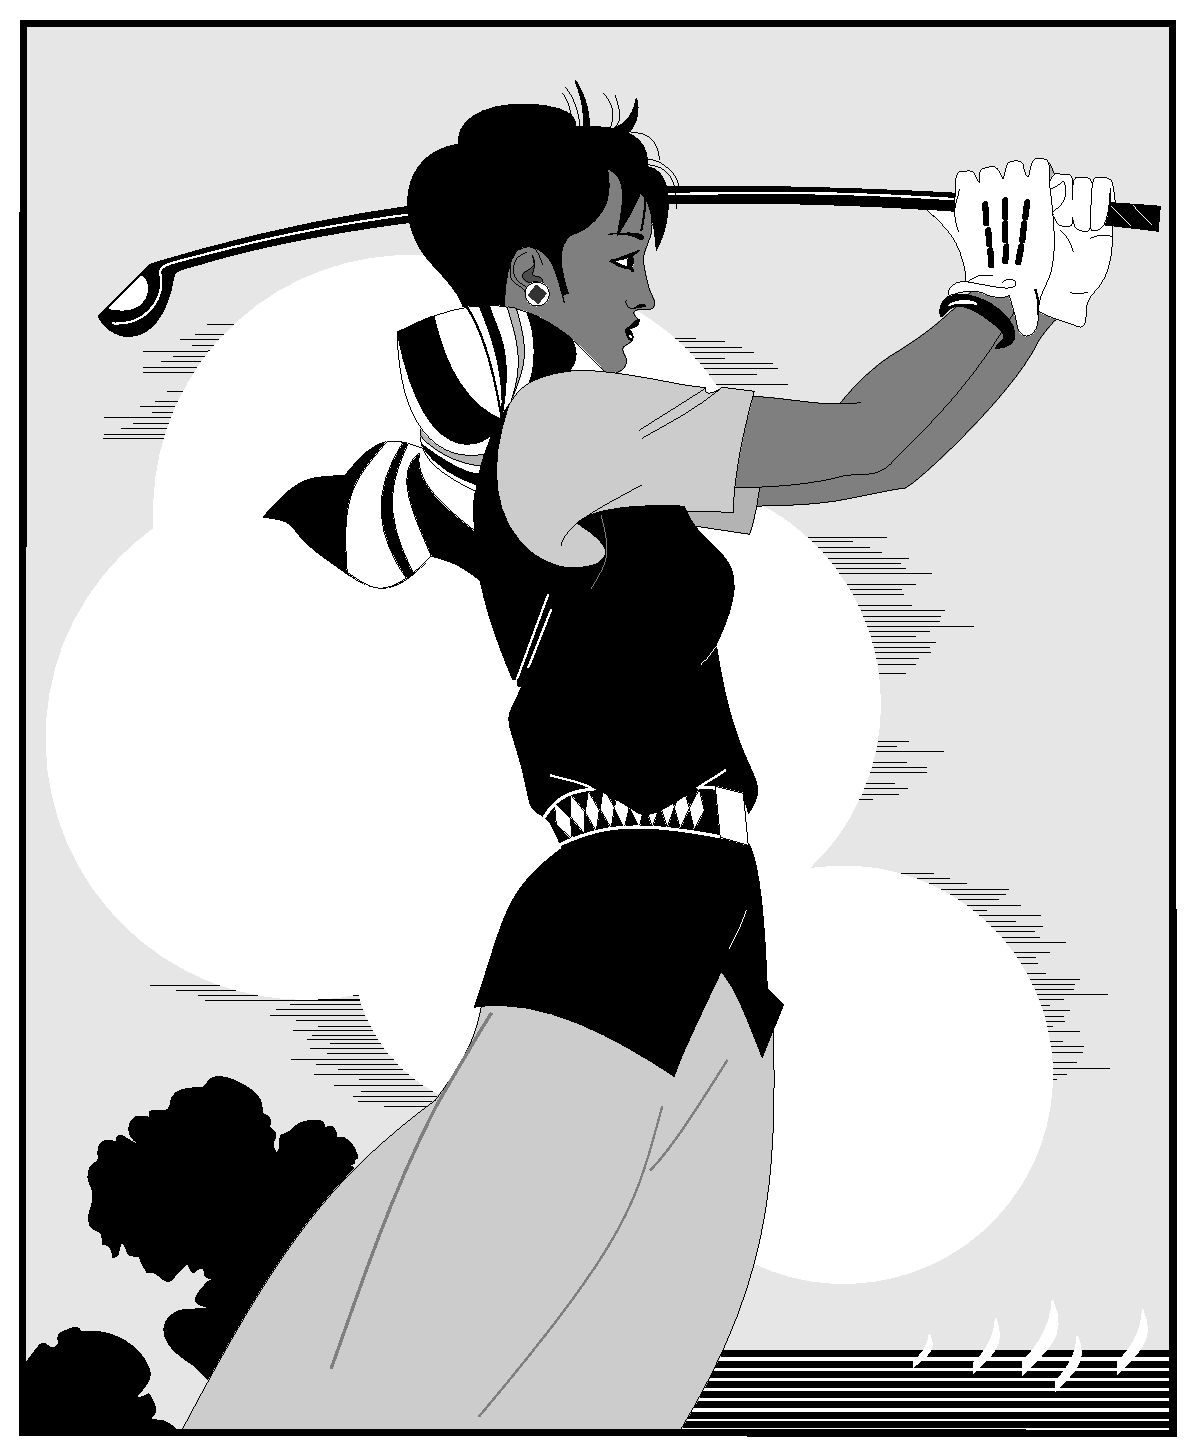
\includegraphics[width = 0.3\textwidth]{golfer}
\caption{打高尔夫球的人}
\label{fig:golfer}
\end{figure}

\begin{code}
\begin{figure}[htbp]
\centering
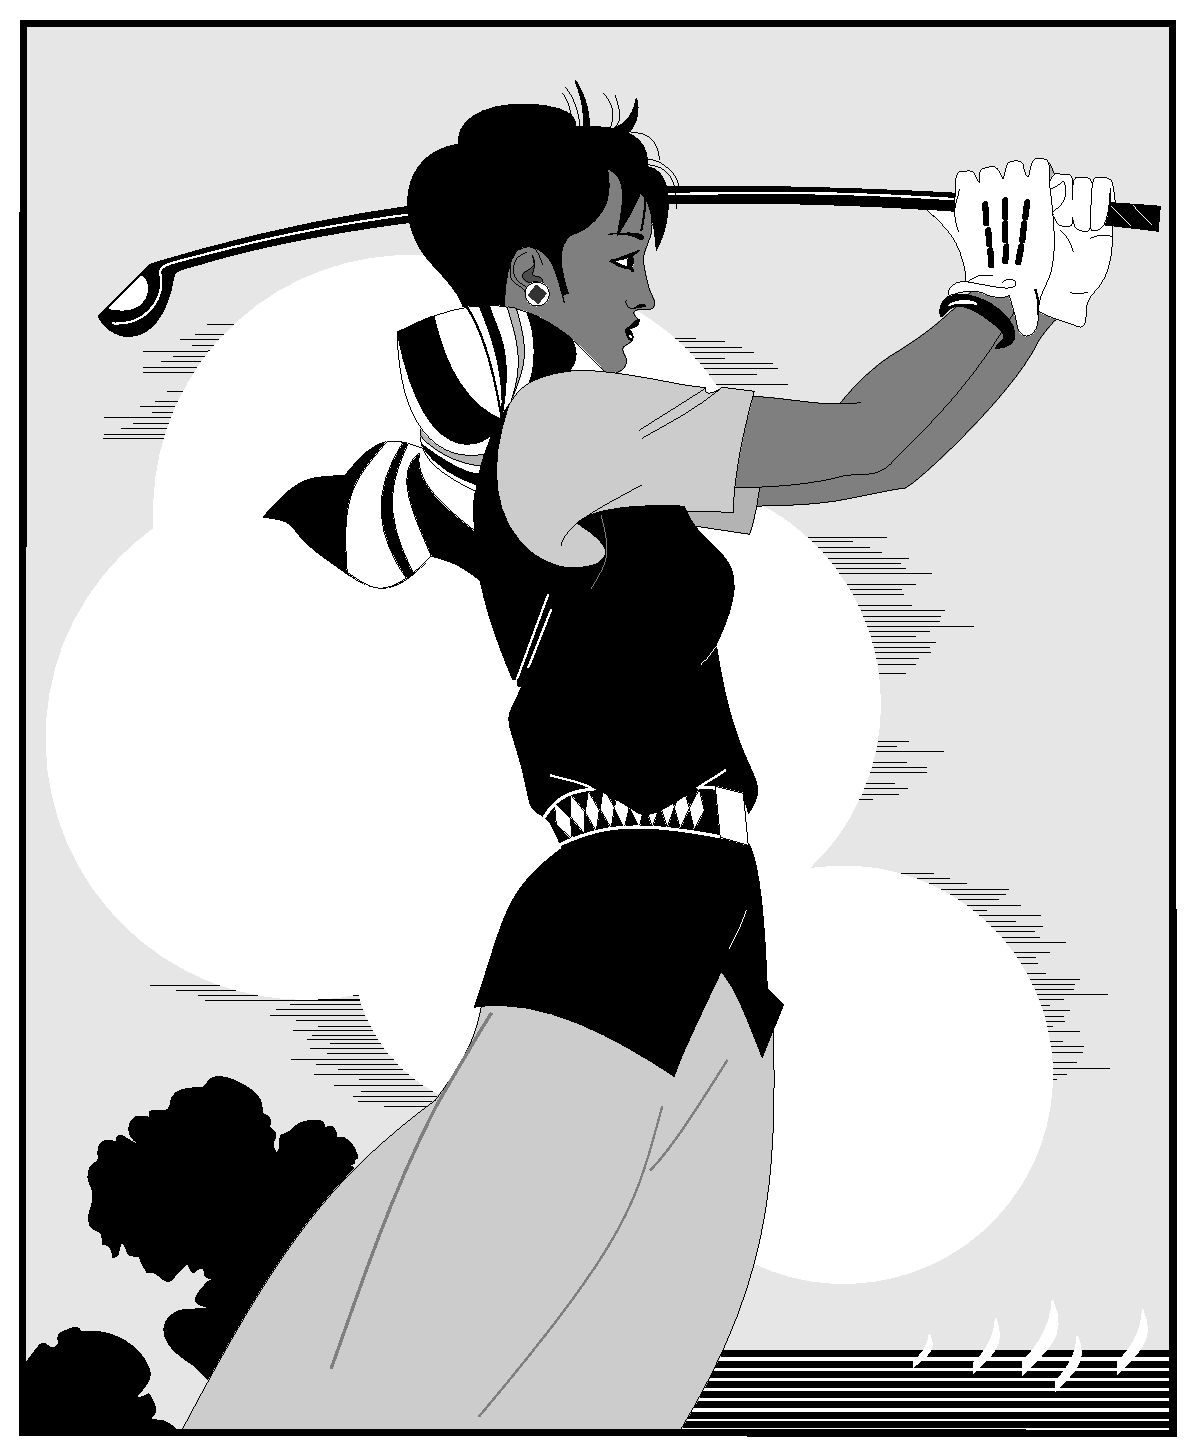
\includegraphics[width=0.3\textwidth]{golfer}
\caption{打高尔夫球的人}
\label{fig:golfer}
\end{figure}
\end{code}

上述代码中,\verb|[htbp]| 选项用来指定插图排版的理想位置,这几个字母分别代表
~here、top、bottom、float page,也就是固定位置、页顶、页尾、单独的浮动页。可
以使用这几个字母的任意组合,一般不推荐单独使用 \verb|[h]|。如果要强制固定浮动
图形的位置,还可以用 \textbf{float} 宏包的 \verb|[H]| 选项。

\verb|\centering| 用来使插图居中,\verb|\caption| 命令设置插图标题,\LaTeX~会
自动给浮动环境的标题加上编号。注意 \verb|label| 应放在 \verb|caption| 之后,否
则引用时指向的是前一个插图。

\subsection{插入多幅图形}

\subsubsection*{并排摆放,共享标题}

当我们需要两幅图片并排摆放,并共享标题时,可以在 \texttt{figure} 环境中使用两个
\verb|\includegraphics| 命令,如图~\ref{fig:fanqingfuming}~所示。

\begin{code}
\begin{figure}[htbp]
\centering

\includegraphics[width=0.3\textwidth]{qingming}
\hspace{36pt}

\includegraphics[width=0.3\textwidth]{fanfu}
\caption{反清复明}
\label{fig:fanqingmuming}
\end{figure}
\end{code}

\begin{figure}[htbp]
\centering

\includegraphics[width=0.3\textwidth]{qingming}
\hspace{36pt}

\includegraphics[width=0.3\textwidth]{fanfu}
\caption{反清复明}
\label{fig:fanqingfuming}
\end{figure}

\subsubsection*{并排摆放,各有标题}

如果想要两幅并排的图片各有自己的标题,可以在 \texttt{figure} 环境中使用两个
 \texttt{minipage} 环境,每个环境里插入一个图,如图~\ref{fig:qingming}~和
~\ref{fig:fanfu}~所示。

\begin{code}
\begin{figure}[htbp]
\centering
\begin{minipage}[t]{0.3\textwidth}
    \centering
    
\includegraphics[width=\textwidth]{qingming}
    \caption{清明}
    \label{fig:qingming}
\end{minipage}
\hspace{36pt}
\begin{minipage}[t]{0.3\textwidth}
    \centering
    
\includegraphics[width=\textwidth]{fanfu}
    \caption{反复}
    \label{fig:fanfu}
\end{minipage}
\end{figure}
\end{code}

\begin{figure}[htbp]
\centering
\begin{minipage}[t]{0.3\textwidth}
    \centering
    
\includegraphics[width=\textwidth]{qingming}
    \caption{清明}
    \label{fig:qingming}
\end{minipage}
\hspace{36pt}
\begin{minipage}[t]{0.3\textwidth}
    \centering
    
\includegraphics[width=\textwidth]{fanfu}
    \caption{反复}
    \label{fig:fanfu}
\end{minipage}
\end{figure}

\subsubsection*{并排摆放,共享标题,各有子标题}

如果想要两幅并排的图片共享一个标题,并各有自己的子标题,可以使用
\textbf{subfig} 宏包提供的 \verb|\subfloat| 命令,如图~\ref{fig:subfig_a}~和
~\ref{fig:subfig_b}~所示。

\verb|\subfloat| 命令缺少宽度参数。虽然我们可以用 \verb|\hspace| 命令调整子图
的距离,子标题却只能和子图本身一样宽,就会出现折行。

\begin{code}
\begin{figure}[htbp]
\centering
\subfloat[清明]{
    \label{fig:subfig_a}
    
\includegraphics[width=0.3\textwidth]{qingming}
}
\hspace{36pt}
\subfloat[反复]{
    \label{fig:subfig_b}
    
\includegraphics[width=0.3\textwidth]{fanfu}
}
\caption{反清复明}
\end{figure}
\end{code}

每个子图可以有各自的引用,就象这个样子:\ref{fig:subfig_a}、
\ref{fig:subfig_b}。

\begin{figure}[htbp]
\centering
\subfloat[清明]{
    \label{fig:subfig_a}
    
\includegraphics[width=0.3\textwidth]{qingming}
}
\hspace{36pt}
\subfloat[反复]{
    \label{fig:subfig_b}
    
\includegraphics[width=0.3\textwidth]{fanfu}
}
\caption{反清复明}
\end{figure}

\subsubsection*{改进的子图方法}

为了避免子标题折行,我们可以在 \verb|\subfloat| 里再嵌套个 \verb|minipage|,因
为后者是有宽度的,如图~\ref{fig:improved_subfig_a}~和
~\ref{fig:improved_subfig_b}~所示。

\begin{code}
\begin{figure}[htbp]
\centering
\subfloat[清明]{
\label{fig:improved_subfig_a}
\begin{minipage}[t]{0.3\textwidth}
    \centering
    
\includegraphics[width=\textwidth]{qingming}
\end{minipage}
}
\hspace{36pt}
\subfloat[反复]{
\label{fig:improved_subfig_b}
\begin{minipage}[t]{0.3\textwidth}
    \centering
    
\includegraphics[width=\textwidth]{fanfu}
\end{minipage}
}
\caption{反清复明}
\end{figure}
\end{code}

\begin{figure}[htbp]
\centering
\subfloat[清明]{
\label{fig:improved_subfig_a}
\begin{minipage}[t]{0.3\textwidth}
    \centering
    
\includegraphics[width=\textwidth]{qingming}
\end{minipage}
}
\hspace{36pt}
\subfloat[反复]{
\label{fig:improved_subfig_b}
\begin{minipage}[t]{0.3\textwidth}
    \centering
    
\includegraphics[width=\textwidth]{fanfu}
\end{minipage}
}
\caption{反清复明}
\end{figure}

\section{表格示例}
\label{sec:table}

模板中关于表格的宏包有四个:\textbf{tabularx}、\textbf{multirow}、
%\textbf{slashbox}、\textbf{array}
\textbf{longtable} 和\textbf{booktabs}。长表格还可以用\textbf{supertabular},
可以方便地在表格下方加入脚注。

\subsection{普通表格的绘制方法}

\texttt{table} 环境是一个将表格嵌入文本的浮动环境,其标题和交叉引用的用法类似
于上一节提到的图形浮动环境 \texttt{figure}。该环境提供了最简单的表格功能。它
用 \verb|\hline| 命令表示横线,\verb&|& 表示竖线;用 \verb|&| 来分列,用
\verb|\\| 来换行;每列可以采用居中、居左、居右等横向对齐方式,分别用 \verb|l|
、\verb|c|、\verb|r| 来表示。

科技文献中常使用三线表格,因此需要调用 \textbf{booktabs} 宏包,三条横线就分别
用 \verb|\toprule|、\verb|\midrule|、\verb|\bottomrule| 等命令表示。其标准格
式如表~\ref{table1}~所示。

\begin{table}[htbp]
\caption{文献类型和标识代码}
\label{table1}
\centering
\begin{tabular}{cccc}
\toprule
文献类型 & 标识代码 & 文献类型 & 标识代码\\
\midrule
普通图书 & M &  会议录 & C\\
汇编 & G & 报纸 & N\\
期刊 & J & 学位论文 & D\\
报告 & R & 标准 & S\\
专利 & P & 数据库 & DB\\
计算机程序 & CP & 电子公告 & EB\\
\bottomrule
\end{tabular}
\end{table}

绘制该表格的代码如下:
\begin{code}
\begin{table}[htbp]
\caption{表格标题}
\label{标签名}
\centering
\begin{tabular}{cc...c}
\toprule
表头第1个格   & 表头第2个格   & ... & 表头第n个格  \\
\midrule
表中数据(1,1) & 表中数据(1,2) & ... & 表中数据(1,n)\\
表中数据(2,1) & 表中数据(2,2) & ... & 表中数据(2,n)\\
...................................................\\
表中数据(m,1) & 表中数据(m,2) & ... & 表中数据(m,n)\\
\bottomrule
\end{tabular}
\end{table}
\end{code}

\subsection{长表格的绘制方法}

长表格是当表格在当前页排不下而需要转页接排的情况下所采用的一种表格环境。若长
表格仍按照普通表格的绘制方法来获得,其所使用的 \verb|table| 浮动环境无法实现
表格的换页接排功能,表格下方过长部分会排在表格第1页的页脚以下。

% \textbf{supertabular} 宏包提供一个 \texttt{supertabular} 环境,是对
% \texttt{tabular} 环境的扩充。它能不断地计算表格长度,当排版到页面底部时,自动
% 结束 \texttt{tabular} 环境,而在下一页再自动生成一个新的 \texttt{tabular} 环境
% ,将剩余表格放入其中。使用该宏包排版长表格时,要用所提供的生成命令专门设计表头
% ,具体方法如下:
% 
% \begin{code}
% \begin{center}
% \tablefirsthead{\toprule 表头第1个格 & 表头第2个格 & ... & 表头第n个格\\
  % \midrule}
% \tablehead{\multicolumn{n}{c}{表~\thetable(续表)}\\
  % \toprule 表头第1个格 & 表头第2个格 & ... & 表头第n个格\\ \midrule}
% \tabletail{\bottomrule
  % \multicolumn{n}{r}{续下页}\\}
% \tablelasttail{\bottomrule}
% \tablecaption{表格标题}\label{标签名}
% \begin{supertabular}{cc...c}
% 表中数据(1,1) & 表中数据(1,2) & ... & 表中数据(1,n)\\
% 表中数据(2,1) & 表中数据(2,2) & ... & 表中数据(2,n)\\
% ...................................................\\
% 表中数据(m,1) & 表中数据(m,2) & ... & 表中数据(m,n)\\
% \end{supertabular}
% \end{center}
% \end{code}
% 
% \verb|\tablehead| 命令描述的是第2页及其之后各页的标题或表头;
% \verb|\tablefirsthead| 命令描述的是第1页的标题和表头,若无此命令,则第1页
% 的表头和标题由 \verb|\tablehead| 命令确定;同理,\verb|\tabletail| 命令描述
% 的是除最后一页之外每页的表格底部内容;\verb|\tablelasttail| 之前的文字描述的是
% 最后一页的表格底部内容,若无此命令,则最后一页表格底部内容由 \verb|\tabletail|
% 命令确定。所绘制的长表格的格式如表~\ref{table2}~所示。
\begin{longtable}{l@{\hspace{6.5mm}}l@{\hspace{5.5mm}}l}
\multicolumn{3}{c}{续表~\thetable\hskip1em 中国省级行政单位一览}\\
\toprule 名称 & 简称 & 省会或首府  \\ \midrule
\endhead
\caption{中国省级行政单位一览}
\label{table2}\\
\toprule 名称 & 简称 & 省会或首府  \\ \midrule
\endfirsthead
\bottomrule
\multicolumn{3}{r}{续下页}\\
\endfoot
\bottomrule
\endlastfoot
北京市 & 京 & 北京\\
天津市 & 津 & 天津\\
河北省 & 冀 & 石家庄市\\
山西省 & 晋 & 太原市\\
内蒙古自治区 & 蒙 & 呼和浩特市\\
辽宁省 & 辽 & 沈阳市\\
吉林省 & 吉 & 长春市\\
黑龙江省 & 黑 & 哈尔滨市\\
上海市 & 沪/申 & 上海\\
江苏省 & 苏 & 南京市\\
浙江省 & 浙 & 杭州市\\
安徽省 & 皖 & 合肥市\\
福建省 & 闽 & 福州市\\
江西省 & 赣 & 南昌市\\
山东省 & 鲁 & 济南市\\
河南省 & 豫 & 郑州市\\
湖北省 & 鄂 & 武汉市\\
湖南省 & 湘 & 长沙市\\
广东省 & 粤 & 广州市\\
广西壮族自治区 & 桂 & 南宁市\\
海南省 & 琼 & 海口市\\
重庆市 & 渝 & 重庆\\
四川省 & 川/蜀 & 成都市\\
贵州省 & 黔/贵 & 贵阳市\\
云南省 & 云/滇 & 昆明市\\
西藏自治区 & 藏 & 拉萨市\\
陕西省 & 陕/秦 & 西安市\\
甘肃省 & 甘/陇 & 兰州市\\
青海省 & 青 & 西宁市\\
宁夏回族自治区 & 宁 & 银川市\\
新疆维吾尔自治区 & 新 & 乌鲁木齐市\\
香港特别行政区 & 港 & 香港\\
澳门特别行政区 & 澳 & 澳门\\
台湾省 & 台 & 台北市\\
北京市 & 京 & 北京\\
天津市 & 津 & 天津\\
河北省 & 冀 & 石家庄市\\
山西省 & 晋 & 太原市\\
内蒙古自治区 & 蒙 & 呼和浩特市\\
辽宁省 & 辽 & 沈阳市\\
吉林省 & 吉 & 长春市\\
黑龙江省 & 黑 & 哈尔滨市\\
上海市 & 沪/申 & 上海\\
江苏省 & 苏 & 南京市\\
浙江省 & 浙 & 杭州市\\
安徽省 & 皖 & 合肥市\\
福建省 & 闽 & 福州市\\
江西省 & 赣 & 南昌市\\
山东省 & 鲁 & 济南市\\
河南省 & 豫 & 郑州市\\
湖北省 & 鄂 & 武汉市\\
湖南省 & 湘 & 长沙市\\
广东省 & 粤 & 广州市\\
广西壮族自治区 & 桂 & 南宁市\\
海南省 & 琼 & 海口市\\
重庆市 & 渝 & 重庆\\
四川省 & 川/蜀 & 成都市\\
贵州省 & 黔/贵 & 贵阳市\\
云南省 & 云/滇 & 昆明市\\
西藏自治区 & 藏 & 拉萨市\\
陕西省 & 陕/秦 & 西安市\\
甘肃省 & 甘/陇 & 兰州市\\
青海省 & 青 & 西宁市\\
宁夏回族自治区 & 宁 & 银川市\\
新疆维吾尔自治区 & 新 & 乌鲁木齐市\\
香港特别行政区 & 港 & 香港\\
澳门特别行政区 & 澳 & 澳门\\
台湾省 & 台 & 台北市\\
\end{longtable}
% \begin{center}
% \tablefirsthead{\toprule 名称 & 简称 & 省会或首府  \\ \midrule}
% \tablehead{\multicolumn{3}{c}{续表~\thetable\hskip1em 中国省级行政单位一览}\\
% \toprule 名称 & 简称 & 省会或首府  \\ \midrule}
% \tabletail{\bottomrule
% \multicolumn{3}{r}{续下页}\\}
% \tablelasttail{\bottomrule}
% \tablecaption{中国省级行政单位一览}
% \label{table2}
% \begin{supertabular}{l@{\hspace{6.5mm}}l@{\hspace{5.5mm}}l}
% 北京市 & 京 & 北京\\
% 天津市 & 津 & 天津\\
% 河北省 & 冀 & 石家庄市\\
% 山西省 & 晋 & 太原市\\
% 内蒙古自治区 & 蒙 & 呼和浩特市\\
% 辽宁省 & 辽 & 沈阳市\\
% 吉林省 & 吉 & 长春市\\
% 黑龙江省 & 黑 & 哈尔滨市\\
% 上海市 & 沪/申 & 上海\\
% 江苏省 & 苏 & 南京市\\
% 浙江省 & 浙 & 杭州市\\
% 安徽省 & 皖 & 合肥市\\
% 福建省 & 闽 & 福州市\\
% 江西省 & 赣 & 南昌市\\
% 山东省 & 鲁 & 济南市\\
% 河南省 & 豫 & 郑州市\\
% 湖北省 & 鄂 & 武汉市\\
% 湖南省 & 湘 & 长沙市\\
% 广东省 & 粤 & 广州市\\
% 广西壮族自治区 & 桂 & 南宁市\\
% 海南省 & 琼 & 海口市\\
% 重庆市 & 渝 & 重庆\\
% 四川省 & 川/蜀 & 成都市\\
% 贵州省 & 黔/贵 & 贵阳市\\
% 云南省 & 云/滇 & 昆明市\\
% 西藏自治区 & 藏 & 拉萨市\\
% 陕西省 & 陕/秦 & 西安市\\
% 甘肃省 & 甘/陇 & 兰州市\\
% 青海省 & 青 & 西宁市\\
% 宁夏回族自治区 & 宁 & 银川市\\
% 新疆维吾尔自治区 & 新 & 乌鲁木齐市\\
% 香港特别行政区 & 港 & 香港\\
% 澳门特别行政区 & 澳 & 澳门\\
% 台湾省 & 台 & 台北市\\
% \end{supertabular}
% \end{center}

表格~\ref{table2}~第~2~页的标题和表头是通过代码自动添加上去的。若表格在页面中
的竖直位置发生了变化,其在第~2~页及之后各页的标题和表头位置能够始终处于各页的
最顶部,无需调整。

\subsection{列宽可调表格的绘制方法}

论文中能用到列宽可调表格的情况共有两种,一种是当插入的表格某一单元格内容过长
以至于一行放不下的情况,另一种是当对公式中首次出现的物理量符号进行注释的情况
,这两种情况都需要调用 \textbf{tabularx} 宏包。下面将分别对这两种情况下可调表格的绘制
方法进行阐述。

\subsubsection{表格内某单元格内容过长的情况}

首先给出这种情况下的一个例子如表~\ref{table3}~所示。

\begin{table}[htbp]
\caption{最小的三个正整数的英文表示法}
\label{table3}
\begin{tabularx}{\textwidth}{llX}
\toprule
Value & Name & Alternate names, and names for sets of the given size\\
\midrule
1 & One & ace, single, singleton, unary, unit, unity\\
2 & Two & binary, brace, couple, couplet, distich, deuce, double, doubleton, duad, duality, duet, duo, dyad, pair, snake eyes, span, twain, twosome, yoke\\
3 & Three & deuce-ace, leash, set, tercet, ternary, ternion, terzetto, threesome, tierce, trey, triad, trine, trinity, trio, triplet, troika, hat-trick\\\bottomrule
\end{tabularx}
\end{table}

绘制该表格的代码如下:

\begin{code}
\begin{table}[htbp]
\caption{表格标题}
\label{标签名}
\begin{tabularx}{\textwidth}{l...X...l}
\toprule
表头第1个格   & ... & 表头第X个格   & ... & 表头第n个格  \\
\midrule
表中数据(1,1) & ... & 表中数据(1,X) & ... & 表中数据(1,n)\\
表中数据(2,1) & ... & 表中数据(2,X) & ... & 表中数据(2,n)\\
.........................................................\\
表中数据(m,1) & ... & 表中数据(m,X) & ... & 表中数据(m,n)\\
\bottomrule
\end{tabularx}
\end{table}
\end{code}

\texttt{tabularx} 环境共有两个必选参数:第1个参数用来确定表格的总宽度,这里取
为排版表格能达到的最大宽度——正文宽度 \verb|\textwidth|;第2个参数用来确定每列
格式,其中标为 \verb|X| 的项表示该列的宽度可调,其宽度值由表格总宽度确定。标
为 \verb|X| 的列一般选为单元格内容过长而无法置于一行的列,这样使得该列内容能
够根据表格总宽度自动分行。若列格式中存在不止一个 \verb|X| 项,则这些标为
\verb|X| 的列的列宽相同,因此,一般不将内容较短的列设为 \verb|X| 。标为
\verb|X| 的列均为左对齐,因此其余列一般选为 \verb|l| (左对齐),这样可使得表格
美观,但也可以选为 \verb|c| 或 \verb|r|。

\subsubsection{对物理量符号进行注释的情况}

为使得对公式中物理量符号注释的转行与破折号“\pozhehao ”后第一个字对齐,此处最
好采用表格环境。此表格无任何线条,左对齐,且在破折号处对齐,一共有“式中”二字
、物理量符号和注释三列,表格的总宽度可选为文本宽度,因此应该采用
\texttt{tabularx} 环境。由该环境生成的对公式中物理量符号进行注释的公式如式
(\ref{eq:1})所示。

\begin{equation}
\label{eq:1}
\ddot{\bm{\rho}}-\frac{\mu}{R_t^3}\left(3\bm{R_t}\frac{\bm{R_t\rho}}{R_t^2}-\bm{\rho}\right)=\bm{a}
\end{equation}
\begin{flushleft}
\renewcommand\arraystretch{1.25}
\begin{tabularx}{\textwidth}{@{}>{\normalsize\rm}l@{\quad}>{\normalsize\rm}l@{\pozhehao }>{\normalsize\rm}X@{}}
式中& $\bm{\rho}$ &追踪飞行器与目标飞行器之间的相对位置矢量;\\
&  $\ddot{\bm{\rho}}$&追踪飞行器与目标飞行器之间的相对加速度;\\
&  $\bm{a}$   &推力所产生的加速度;\\
&  $\bm{R_t}$ & 目标飞行器在惯性坐标系中的位置矢量;\\
&  $\omega_{t}$ & 目标飞行器的轨道角速度;\\
&  $\bm{g}$ & 重力加速度,$=\frac{\mu}{R_{t}^{3}}\left(
3\bm{R_{t}}\frac{\bm{R_{t}\rho}}{R_{t}^{2}}-\bm{\rho}\right)=\omega_{t}^{2}\frac{R_{t}}{p}\left(
3\bm{R_{t}}\frac{\bm{R_{t}\rho}}{R_{t}^{2}}-\bm{\rho}\right)$,这里~$p$~是目标飞行器的轨道半通径。
\end{tabularx}\vspace{.5ex}%TODO : 注释内容自动转页接排
\end{flushleft}
% 式中\quad
% \parbox[t][][c]{2em}{
  % $\ddot{\bm{\rho}}$\\
  % $\bm{a}$\\
  % $\bm{R_t}$\\
  % $\omega_{t}$\\
% }
% \parbox[t][][c]{2em}{
  % \pozhehao\\
  % \pozhehao\\
  % \pozhehao\\
  % \pozhehao\\
% }
% \parbox[t][][c]{\textwidth-8em}{
 % 追踪飞行器与目标飞行器之间的相对加速度;\\
 % 推力所产生的加速度;\\
 % 目标飞行器在惯性坐标系中的位置矢量;\\
 % 目标飞行器的轨道角速度;\\}

% 由此方法生成的注释内容应紧邻待注释公式并置于其下方,因此不能将代码放入
% \texttt{table} 浮动环境中。但此方法不能实现自动转页接排,可能会在当前页剩余空
% 间不够时,全部移动到下一页而导致当前页出现很大空白。

其中生成注释部分的代码及其说明如下:
\begin{code}
\begin{tabularx}{\textwidth}{@{}l@{\quad}l@{\pozhehao}X@{}}
式中 & symbol-1 & symbol-1的注释内容;\\
     & symbol-2 & symbol-2的注释内容;\\
     .............................;\\
     & symbol-m & symbol-m的注释内容。
\end{tabularx}
\end{code}

\texttt{tabularx} 环境的第1个参数为正文宽度,第2个参数里面各个符号的意义为:
\begin{itemize}
\item 第1个@{}表示在“式中”二字左侧不插入任何文本,“式中”二字能够在正文中左对
齐,若无此项,则“式中”二字左侧会留出一定的空白;
\item \verb|@{\quad}| 表示在“式中”和物理量符号间插入一个空铅宽度的空白;
\item \verb|@{\pozhehao}| 实现插入破折号的功能;
\item 第2个 \verb|@{}| 表示在注释内容靠近正文右边界的地方能够实现右对齐。
\end{itemize}

% 若想获得绘制表格的更多信息,请参见网络上的~Tables in \LaTeXe: Packages and
% Methods~文档~http://www.tug.org/pracjourn/2007-1/mori/。 

% \begin{table}[htb]
  % \centering
  % \begin{minipage}[t]{0.8\linewidth} % 如果想在表格中使用脚注,minipage是个不错的办法
  % \caption[模板文件]{模板文件。如果表格的标题很长,那么在表格索引中就会很不美
    % 观,所以要像 chapter 那样在前面用中括号写一个简短的标题。这个标题会出现在索
    % 引中。}
  % \label{tab:template-files}
    % \begin{tabular*}{\linewidth}{lp{10cm}}
      % \toprule
      % {\hei 文件名} & {\hei 描述} \\
      % \midrule
      % zzuthesis.cls & 模板类文件。\\
      % zzuthesis.cfg & 模板配置文。\\
      % thubib.bst    & 参考文献 Bibtex 样式文件。\\
      % main.tex      & 主文档。\\
      % Makefile      & Linux 自动处理文件。\footnote{Linux系统自动编译处理。}\\
      % msmake      & Windows 自动处理文件。\footnote{Windows系统自动编译。}\\
      % data\textbackslash & 封面、摘要、符号说明、正文章节、简历、致谢等。\\
      % figures\textbackslash & 文档用到的图片。\\
      % ref\textbackslash & 参考文献数据库。\\
      % \bottomrule
    % \end{tabular*}
  % \end{minipage}
% \end{table}

% 表\ref{tab:template-files} 列举了本模板主要文件及其功能,还展示了如何在表格
% 中正确使用脚注。由于 \LaTeX{} 本身不支持在表格中使用 \verb|\footnote|,所以
% 不得不将表格放在小页中,而且最好将表格的宽度设置为小页的宽度,这样脚注看起
% 来才更美观。

% 我们经常会在表格下方标注数据来源,或者对表格里面的条目进行解释。前面的脚注
% 是一种不错的方法,如果你不喜欢脚注。那么完全可以在表格后面自己写注释,比如
% 表~\ref{tab:tabexamp1}。

% \begin{table}[ht]
  % \centering
  % \caption{复杂表格示例 1}
  % \label{tab:tabexamp1}
  % \begin{minipage}[t]{0.8\textwidth} 
    % \begin{tabularx}{\linewidth}{|l|X|X|X|X|}
      % \hline
 % \multirow{2}*{\backslashbox{x}{y}}  & \multicolumn{2}{c|}{First Half} & \multicolumn{2}{c|}{Second Half}\\\cline{2-5}
      % & 1st Qtr &2nd Qtr&3rd Qtr&4th Qtr \\ \hline
      % East$^{*}$ &   20.4&   27.4&   90&     20.4 \\
      % West$^{**}$ &   30.6 &   38.6 &   34.6 &  31.6 \\ \hline
    % \end{tabularx}\\[2pt]
    % \footnotesize 注:数据来源《\zzuthesis{} 使用手册》。\\
    % *:东部\\
    % **:西部
  % \end{minipage}
% \end{table}

% 此外,表~\ref{tab:tabexamp1} 同时还演示了另外两个功能:1)通过
% \textbf{tabularx} 的\texttt{|X|} 扩展实现表格自动放大;2)通过命令
% \verb|\backslashbox| 在表头部分插入反斜线。

% 浮动体的并排放置一般有两种情况:1)二者没有关系,为两个独立的浮动体;2)二
% 者隶属于同一个浮动体。对表格来说并排表格既可以像表~\ref{tab:parallel1}、表
% ~\ref{tab:parallel2} 使用小页环境,也可以如表~\ref{tab:subtable} 使用子表格
% 来做。

% \begin{table}[ht]
% \noindent\begin{minipage}{0.5\textwidth}
% \centering
% \caption{第一个并排子表格}
% \label{tab:parallel1}
% \begin{tabular}{p{2cm}p{2cm}}
% \toprule[1.5pt]
% 111 & 222 \\\midrule[1pt]
% 222 & 333 \\\bottomrule[1.5pt]
% \end{tabular}
% \end{minipage}
% \begin{minipage}{0.5\textwidth}
% \centering
% \caption{第二个并排子表格}
% \label{tab:parallel2}
% \begin{tabular}{p{2cm}p{2cm}}
% \toprule[1.5pt]
% 111 & 222 \\\midrule[1pt]
% 222 & 333 \\\bottomrule[1.5pt]
% \end{tabular}
% \end{minipage}
% \end{table}

% \begin{table}
% \centering
% \caption{并排子表格}
% \label{tab:subtable}
% \subfloat[第一个子表格]{
% \begin{tabular}{p{2cm}p{2cm}}
% \toprule[1.5pt]
% 111 & 222 \\\midrule[1pt]
% 222 & 333 \\\bottomrule[1.5pt]
% \end{tabular}}\hskip2cm
% \subfloat[第二个子表格]{
% \begin{tabular}{p{2cm}p{2cm}}
% \toprule[1.5pt]
% 111 & 222 \\\midrule[1pt]
% 222 & 333 \\\bottomrule[1.5pt]
% \end{tabular}}
% \end{table}

% 有的同学不想让某个表格或者图片出现在索引里面,那么请使用命令
% \verb|\caption*{}|,这个命令不会给表格编号,也就是出来的只有标题文字而没有“表
% ~XX”,“图~XX”,否则索引里面序号不连续就显得不伦不类,这也是 \LaTeX{} 里星号命
% 令默认的规则。
% 
% \begin{table}[ht]
% \centering
  % \begin{minipage}{0.45\linewidth}
  % \centering
  % \caption*{表~1.111\hskip1em 这是一个手动编号,不出现在索引中的表格。}
  % \label{tab:badtabular}
  % \begin{picture}(150,50)
    % \framebox(150,50)[c]{\zzuthesis}
  % \end{picture}    
  % \end{minipage}\hfill
  % \begin{minipage}{0.45\linewidth}
  % \centering
  % \begin{picture}(150,50)
    % \framebox(150,50)[c]{薛瑞尼}
  % \end{picture}
  % \caption*{Figure~1.111\hskip1em 这是一个手动编号,不出现在索引中的图。}
  % \label{tab:badfigure}
  % \end{minipage}
% \end{table}
% 

\subsection{小页中的脚注}

关于小页中的脚注,请看下面的例子:
 
\begin{minipage}[t]{\linewidth-2\parindent}
柳宗元,字子厚(773-819),河东(今永济县)人\footnote{山西永济水饺。},是唐
代杰出的文学家,哲学家,同时也是一位政治改革家。与韩愈共同倡导唐代古文运动,
并称韩柳\footnote{唐宋八大家之首二位。}。
\end{minipage}\\[-5pt]

\section{数学公式示例}
\label{sec:equation}

\LaTeX{} 的数学公式有两种形式:行间(inline)模式和独立(display)模式。前者是
指在正文中插入数学内容;后者独立排列,可以有或者没有编号。行间公式和无编号独立
公式都有多种输入方法,一般行间公式用 \verb|$|\ldots \verb|$|,无编号独立公式用
\verb|\[|\ldots \verb|\]|。有编号独立公式则需要用 \texttt{equation} 环境。

注意一下公式显示模式的不同,这个公式为行间模式:
$\lim_{n \to \infty} \sum_{k=1}^n \frac{1}{k^2} = \frac{\pi^2}{6}$;下面的公式
是独立模式:
\[\lim_{n \to \infty} \sum_{k=1}^n \frac{1}{k^2} = \frac{\pi^2}{6}\]

\subsection{多行公式}

\textbf{amsmath} 宏包提供了额外的行间独立(display)公式的结构,主要用于一个
公式太长一行放不下,或几个公式需要写成一组的情况,该宏包主要提供以下几个环境
:
\begin{center}
\begin{tabular}[c]{ccccccc}
equation & equation* & align & align* & gather & gather* & split \\
flalign & flalign* & multline & multline* & alignat & alignat* & \\
\end{tabular}
\end{center}

除了 \texttt{split} 外,其余环境均提供带*的版本,不生成公式编号。

% \subsection{矩阵}
% 
% 数学模式下可以用 \verb|array| 环境来生成矩阵,它提供了外部对齐和列对齐的控制参
% 数。外部对齐是指整个矩阵和周围对象的纵向关系,有三种方式:居顶、居中 (缺省) 、
% 居底,分别用 \verb|l、c、r| 来表示;列对齐也有三种方式:居左、居中、居右,分别
% 用 \verb|l、c、r| 表示。\verb|\\| 和 \verb|&| 用来分隔行和列。
% 
% \[\begin{array}{ccc}
% x_1 & x_2 & \dots \\
% x_3 & x_4 & \dots \\
% \vdots & \vdots & \ddots \\
% \end{array}\]

% \verb|amsmath| 有几个类似的环境:\verb|pmatrix、bmatrix、Bmatrix、vmatrix|~和~
% \verb|Vmatrix|,它们和 \verb|array| 的主要区别是会在表两端加上~$()\; []\;
% \{\}\; ||\; \|\|$~等分隔符,其次这些环境没有列对齐方式参数。
% 
% 行间公式可以用 \verb|smallmatrix| 环境来生成排列紧密的小矩阵,如
% $(\begin{smallmatrix} a&b\\c&d \end{smallmatrix})$。
% 

\subsubsection{长公式}

对于多行不需要对齐的长公式,我们可以用 \texttt{multline} 环境。
\begin{multline}
\framebox[.65\columnwidth]{A}\\
\framebox[.5\columnwidth]{B}\\
\shoveright{\framebox[.5\columnwidth]{C}}\\
\framebox[.65\columnwidth]{D}
\end{multline}

其代码如下:
\begin{code}
\begin{multline}
\framebox[.65\columnwidth]{A}\\
\framebox[.5\columnwidth]{B}\\
\shoveright{\framebox[.tt\columnwidth]{C}}\\
\framebox[.65\columnwidth]{D}
\end{multline}
\end{code}

\texttt{multline} 环境用于单行放不下的长公式,其第一行及最后一行分别居左、居右
对齐,两端均缩进距离 \verb|\multlinegap|;其它行则默认居中排布,但可以用个命令
\verb|\shoveleft|、\verb|\shoveright| 分别使居左或居右排布。

需要对齐的长公式可以用 \texttt{split} 环境,它本身不能单独使用,因此也称作次环境
,必须包含在 \texttt{equation} 或其它数学环境内。\texttt{split} 环境用 \verb|\\| 
和 \verb|&| 来分行和设置对齐位置。
\begin{equation}
\begin{split}
H_c&=\frac{1}{2n} \sum^n_{l=0}(-1)^{l}(n-{l})^{p-2}
\sum_{l _1+\dots+ l _p=l}\prod^p_{i=1} \binom{n_i}{l _i}\\
&\quad\cdot[(n-l)-(n_i-l_i)]^{n_i-l_i}\cdot
\Bigl[(n-l)^2-\sum^p_{j=1}(n_i-l_i)^2\Bigr].
\end{split}
\label{eqn:barwq}
\end{equation}

\subsubsection{公式组}

不需要对齐的公式组用 \texttt{gather} 环境,该环境中的公式均居中排布,各公式间用
\verb|\\| 分开;需要对齐的用 \texttt{align},在该环境中使用 \verb|\text| 命令可
以生成对单独公式的注释。
\begin{gather}
  first equation\\
  \begin{split}
    second & equation\\
           & on twolines
  \end{split}
\end{gather}

\begin{align}
 x & = y_1-y_2+y_3-y_5+y_8-\dots && \text{by \eqref{eqn:barwq}}\\
   & = y'\circ y^*               && \text{by \eqref{eqn:barwq}}\\
   & = y(0) y'                   && \text{by Axiom 1.}
\end{align}

就像单独的行间公式一样,使用 \texttt{gather}、\texttt{align} 和
\texttt{alignat} 环境生成的公式组中的每个公式也都是占据整个文本的宽度,因此
这样的公式组两侧不能再添加其它内容,比如大括号等。不过相应地用
\texttt{gathered}、\texttt{aligned} 和 \texttt{alignedat} 环境则生成仅占据
实际公式宽度的公式组。
\begin{equation*}
\left. \begin{aligned}
  \bm{B'}&=-\bm{\partial}\times \bm{E},\\
  \bm{E'}&=\bm{\partial}\times \bm{B} - 4\pi j,
\end{aligned}
\right\}
\qquad \text{Maxwell's equations}
\end{equation*}

有多种条件的公式组用 \texttt{cases} 次环境。
\[ P_{r-j}=\begin{cases}
  0& \text{if $r-j$ is odd},\\
  r!\,(-1)^{(r-j)/2}& \text{if $r-j$ is even}.
\end{cases} \]

这里仅简单介绍了 \textbf{amsmath} 的功能,更详尽的说明可参见该宏包的文档。

\subsection{定理和证明}

\zzuthesis{} 定义了常用的数学环境:
\begin{center}
\begin{tabular}{*{7}{l}}\hline
  axiom & theorem & definition & proposition & lemma & conjecture &\\
  公理 & 定理 & 定义 & 命题 & 引理 & 猜想 &\\\hline
  proof & corollary & example & exercise & assumption & remark & problem \\
  证明 & 推论 & 例子& 练习 & 假设 & 注释 & 问题\\\hline
\end{tabular}
\end{center}

以上环境的定义采用 \textbf{amsthm} 宏包提供的 \verb|\newtheorem| 命令,其语法
如下:

\begin{code}
\newtheorem{环境名}[编号延续]{显示名}[编号层次]
\end{code}

% 下面的代码定义了四个环境:定义、定理、引理和推论,它们都在一个 \verb|chapter| 
% 内编号,而引理和推论会延续定理的编号。
% \begin{code}
% \newtheorem{definition}{定义}[chapter]
% \newtheorem{theorem}{定理}[chapter]
% \newtheorem{lemma}{引理}[chapter]
% \newtheorem{corollary}[theorem]{推论}
% \end{code}
% 
% 定义了上述环境之后,我们就可以象下面这样使用它们。
下面是应用示例:
\begin{definition}
Java是一种跨平台的编程语言。
\end{definition}

\begin{theorem}
咖啡因会使人的大脑兴奋。
\end{theorem}

\begin{lemma}
茶和咖啡都会使人兴奋。
\end{lemma}

\begin{corollary}
晚上喝咖啡会导致失眠。
\end{corollary}

\texttt{proof} 环境可以用来输入下面这样的证明,它会在证明结尾输入一个~QED~符号
\footnote{拉丁语~quod erat demonstrandum~的缩写。}。

\begin{proof}[命题“物质无限可分”的证明]
一尺之棰,日取其半,万世不竭。
\end{proof}

% \begin{theorem}
% 如果函数$f(x)$满足
% \begin{enumerate}
% \item 在闭区间$[a,b]$上连续;
% \item 在开区间$(a,b)$内可导;
% \item 在区间端点处的函数值相等,即$f(a)=f(b)$,
% \end{enumerate}
% 那么在$(a,b)$内至少有一点$\xi(a<\xi<b)$,使得$f^\prime(\xi)=0$。这个定理称之为%
% \textbf{罗尔定理}。
% \label{the:rolle}
% \end{theorem}
% 
% 贝叶斯公式如式~(\ref{equ:bayes}),其中 $p(y|\mathbf{x})$ 为后验;
% $p(\mathbf{x})$ 为先验;分母 $p(\mathbf{x})$ 为归一化因子。
% \begin{equation}
% \label{equ:bayes}
% p(y|\mathbf{x}) = \frac{p(\mathbf{x},y)}{p(\mathbf{x})}=
% \frac{p(\mathbf{x}|y)p(y)}{p(\mathbf{x})} 
% \end{equation}
% 
% 再看一个 \textbf{amsmath} 的例子:
% \newcommand{\envert}[1]{\left\lvert#1\right\rvert} 
% \begin{equation}\label{detK2}
% \det\mathbf{K}(t=1,t_1,\dots,t_n)=\sum_{I\in\mathbf{n}}(-1)^{\envert{I}}
% \prod_{i\in I}t_i\prod_{j\in I}(D_j+\lambda_jt_j)\det\mathbf{A}
% ^{(\lambda)}(\overline{I}|\overline{I})=0.
% \end{equation} 
% 
% 多级规划的例子:
% \begin{equation}\label{bilevel}
% \left\{\begin{array}{l}
% \max\limits_{{\mbox{\footnotesize\boldmath $x$}}} F(x,y_1^*,y_2^*,\cdots,y_m^*)\\[0.2cm]
% \mbox{subject to:}\\[0.1cm]
% \qquad G(x)\le 0\\[0.1cm]
% \qquad(y_1^*,y_2^*,\cdots,y_m^*)\mbox{ solves problems }(i=1,2,\cdots,m)\\[0.1cm]
% \qquad\left\{\begin{array}{l}
    % \max\limits_{{\mbox{\footnotesize\boldmath $y_i$}}}f_i(x,y_1,y_2,\cdots,y_m)\\[0.2cm]
    % \mbox{subject to:}\\[0.1cm]
    % \qquad g_i(x,y_1,y_2,\cdots,y_m)\le 0.
    % \end{array}\right.
% \end{array}\right.
% \end{equation}
% 
% \begin{theorem}
% 设$f:[a,b]\rightarrow \mathbf R$为一连续函数,$g:[a,b]\rightarrow \mathbf R$为
% 一正的可积函数,那么存在一点$\xi\in [a,b]$使得:
% \[\int_a^b f(x)g(x)\,dx= f(\xi)\int_a^b g(x)\,dx\]
% \end{theorem}
% 
% \begin{proof}
% 
% 因为f是闭区间上的连续函数,f取得最大值M和最小值m。于是:
% \[mg(x)\leq f(x)g(x)\leq Mg(x)\]
% 
% 对不等式求积分,我们有:
% \[m\int_a^b g(x)\,dx\leq \int_a^b f(x)g(x)\,dx \leq M\int_a^b
% g(x)\,dx\]
% 若$\int_a^b g(x)\,dx=0$,则$\int_a^b f(x)g(x)\,dx=0$,$\xi$可取$[a,b]$上任一点
% 。
% 
% 设 $\int_a^b g(x)\,dx>0$,那么:
% \[m\leq \frac{\int_a^b f(x)g(x)\,dx}{\int_a^b g(x)\,dx}\leq M\]
% 
% 因为 $m\leq f(x)\leq M$是连续函数,则必存在一点 $\xi\in [a,b]$,使得:
% \begin{equation}
% f(\xi)= \frac{\int_a^b f(x)g(x)\,dx}{\int_a^b g(x)\,dx}
% \label{eqn:lagrange1}
% \end{equation}
% \end{proof}
% 
% \begin{corollary}
% 在式~\ref{eqn:lagrange1}中令$g(x)=1$,则可得出:
% 
% 设$f:[a,b]\rightarrow \mathbf R$为一连续函数,则$\exists\xi\in [a,b]$,使:
% \begin{equation}
% f(\xi)= \frac{\int_a^b f(x)\,dx}{b-a}
% \label{eqn:lagrange2}
% \end{equation}
% \end{corollary}
% 
% \begin{example}
  % 大家来看这个例子。
% \begin{equation}
% \label{ktc}
% \left\{\begin{array}{l}
% \nabla f({\mbox{\boldmath $x$}}^*)-\sum\limits_{j=1}^p\lambda_j\nabla g_j({\mbox{\boldmath $x$}}^*)=0\\[0.3cm]
% \lambda_jg_j({\mbox{\boldmath $x$}}^*)=0,\quad j=1,2,\cdots,p\\[0.2cm]
% \lambda_j\ge 0,\quad j=1,2,\cdots,p.
% \end{array}\right.
% \end{equation}
% \end{example}
% 
% \begin{exercise}
% 请列出 Andrew S. Tanenbaum 和 W. Richard Stevens 的所有著作。
% \end{exercise}
% 
% \begin{conjecture}
% \textit{Poincare Conjecture} If in a closed three-dimensional space, any
% closed curves can shrink to a point continuously, this space can be deformed
% to a sphere.
% \end{conjecture}
% 
% \begin{problem}
 % 回答还是不回答,是个问题。 
% \end{problem}



%%%%%%%%%%%%%%%%%%%%%%%%%%%%%%%%%%%%%%%%%%%%%%%%%%
%% 文后
%%%%%%%%%%%%%%%%%%%%%%%%%%%%%%%%%%%%%%%%%%%%%%%%%%
\backmatter

\bibliographystyle{gbt-7714-2015-numerical}
\bibliography{ref/test}%参考文献

\makeatletter%致谢,研究生论文中在参考文献后,附录前
\ifzzu@bachelor\else
  %%================================================
%% Filename: ack.tex
%% Encoding: UTF-8
%% Author: Yuan Xiaoshuai - yxshuai@gmail.com
%% Created: 2012-01-12 18:09
%% Last modified: 2016-08-28 21:05
%%================================================
\begin{ack}

韶华易逝,光阴荏苒,余自入渝倏忽而又三年矣。曩者,离鲁地,弃吴越奔巴蜀,恢恢乎
若漏网之鲫,惶惶乎似惊弓之鸟,几无容身之地。幸遇刘徐二相荐,得拜于恩师魏公门下
,而今已历六秋。先生治学严谨,博通中外,蔚为家,研习学术,废寝忘食,已臻忘我之
境界。犹忆当年,乍入门墙,耻无寸功先生不以余愚钝,委以重托,是以矢勤矢勇,思惟
速战,毋负所托。然欲速不心忧如焚。全赖先生数次点拨,每自躬亲,甚于子夜,共为进
退,方有所成。于缀词成文,苦心孤诣,字斟句酌,独具匠心,深为叹服,并于耳提面命
之际益良多。先生之德才,若高山仰止,亦非庸庸如吾辈者所能望其项背。每至周常言:
“修身者智之府也,爱施者仁之端也,取予者义之符也,耻辱者勇之决也立名者行之极也
。凡此五者,皆安身立命之本,不可偏废。”言之谆谆,听之诚若醍醐灌顶。退而思之,
果斯然也,大为拜服。兼之师母,待余恩厚,视若螟多得给养,感激涕零。余素朴陋,尚
无剖符丹书之功,反受此殊遇,非结草衔不可报也!今虽即辞师门,必常怀乌鸟之情,反
哺之心,诚不失其望也!

师门同侪,学强张骞,皆忠义之士,情同手足;乐至四国,许都耀琼,此良实,多蒙所助
;兰莉二姊,性行淑均,爱如姐弟。其他诸君,皆为志虑忠纯士,多有广益。区区不才,
有何德能,安得广助若此?感荷之心,亦自拳拳。实验中曾多次求教于杨(明莉)、杜(
军)二老师,受益匪浅;中心实验室(光辉)、鲜(晓红)二位老师及刘姊渝萍为实验工
作大开方便之门,谨表谢忱家中上至期颐之祖母,中至慈爱之父母、姊姊,下至始龀之甥
男,均不遗力以支持,融融亲情,曷其幸甚!谨撰此文,鱼传尺素,答报椿萱!

嗟乎!聚散无常,盛况难再;书不尽意,略陈固陋。临别赠言,幸承恩于公;登高作赋,
是所望于群贤。斗胆献拙,情之不已;一言均赋,四韵俱成。洒陵江,以酹逝去之岁月。

\begin{center}
西入渝州已六霜,貔貅帐里铸鱼肠。\\
书山文海研学术,翠袖红巾戏皮黄。\\
莫叹时舛惟虎踞,且图运转季鹰扬。\\
今朝叩别师尊去,一片丹心化碧江。
\footnote{重庆大学化工博士季孟波学位论文《抗溺水性气体多孔电极的研究》致谢词}
\end{center}

\end{ack}

\fi
\makeatother

% 附录
% 本科生论文三个附录,分别是附表,外文翻译和外文原文
% 研究生论文无具体要求
\begin{appendix}
  %%================================================
%% Filename: app01.tex
%% Encoding: UTF-8
%% Created: 2017-05-20
%%================================================
\newgeometry{left=2cm,top=3cm,bottom=2cm,right=2cm,includefoot}
\chapter{表格附件}
\section*{\centering\sanhao\hei 毕业设计(论文)任务书}
\addcontentsline{toc}{section}{附表~1:毕业设计(论文)任务书}
\vspace*{.5ex}
\begin{center}
\renewcommand\arraystretch{1.25}
\newcommand{\minitab}[2][>{\rm}m{2em}]{\begin{tabular}{#1}#2\end{tabular}}
\begin{tabularx}{\textwidth}{|>{\centering\rm}m{2em}|X|}
\hline
\multirow{6}{2em}{\minitab{课\\题\\情\\况}} &
\minitab[>{\centering\rm}m{7em}|c]{课题名称 & } \\ 
\cline{2-2}
&\minitab[>{\centering\rm}m{7em}|>{\centering}m{3em}|>{\centering\rm}m{2em}|>{\centering}m{2em}|>{\centering\rm}m{2em}|>{\centering}m{2em}|>{\centering\rm}m{3em}|X]{
教师姓名 & & 职称 & & 学位 & & 教研室 & }\\
\cline{2-2}
 & \minitab[>{\centering\rm}m{7em}|>{\rm}c]{课题来源 & A. 科研 \checkmark\quad B. 生产\quad C. 教学\quad D. 其它}\\
\cline{2-2}
 &\minitab[>{\centering\rm}m{7em}|>{\centering\rm}m{12em}|>{\centering\rm}m{4em}|X]{课题类别 & A. 设计\quad B. 论文 \checkmark & 实施地点 & }\\
\cline{2-2}
 &
\minitab[>{\centering\rm}m{7em}|>{\centering}m{12em}|>{\centering\rm}m{4em}|>{\rm}X]{起止时间 & 2011 年 11 月 $\sim$ 2012 年 6 月 & 上机时数 & }\\
\cline{2-2}
 & \minitab[>{\centering\rm}m{7em}|>{\rm}X]{拟指导的学生数 & \minitab[c|>{\rm}c|c]{1 人 & 对学生的特殊要求 & 基础知识扎实,动手能力较强}}\\
\hline
{\renewcommand\arraystretch{1}\minitab{主\\要\\研\\究\\内\\容}}&{
\vspace*{-7ex}\begin{minipage}[t][10ex][s]{.9\textwidth}\hspace{2em}
主要研究内容
\end{minipage}
}\\
\hline
{\renewcommand\arraystretch{1}\minitab{目\\标\\和\\要\\求}} &{
\vspace*{-6.4ex}\begin{minipage}[t][10ex][s]{.9\textwidth}\hspace{2em}
目标和要求
\end{minipage}
}\\
\hline
{\renewcommand\arraystretch{1}\minitab{特\\色}} & 特色\\
\hline
{成果形式} & 论文\\
\hline
{成果价值} & 有一定的学术价值\\
\hline
{\renewcommand\arraystretch{1}\minitab{科\\室\\审\\题\\意\\见}} &
{\rm\vspace*{2.4ex}\hbox{\hspace{.2\textwidth}负责人签字:\hspace{8em}年\hspace{2em}月\hspace{2em}日}}
\\
\hline
{\renewcommand\arraystretch{1}\minitab{学\\院\\审\\批\\意\\见}} &
{\rm\vspace*{2.4ex}\hbox{\hspace{.2\textwidth}主管院长签字:\hspace{7em}年\hspace{2em}月\hspace{2em}日}}
\\
\hline
\end{tabularx}
\end{center}

\newpage
\renewcommand\arraystretch{1.25}
\section*{\centering\song\sanhao 郑州大学毕业论文开题报告表}
\addcontentsline{toc}{section}{附表~2:郑州大学毕业论文开题报告表}
\begin{center}
\vspace*{0.5ex}
\hfil 院(系):\texttt{物理工程学院}\hspace{15em} 类别:论文\hfil\hfil
\vspace*{0.5ex}

\begin{tabularx}{\textwidth}{|>{\centering\rm}p{.12\textwidth}|>{\centering}p{.12\textwidth}|>{\centering\rm}p{.08\textwidth}|>{\centering}p{.15\textwidth}|>{\centering\rm}p{.05\textwidth}|Z|}
\hline
课题名称 & \multicolumn{5}{c|}{} \\
\hline
导师姓名 & & 职\quad{}称 & \multicolumn{3}{c|}{} \\
\hline
学生姓名 & & 学\quad{}号 & & 专业 & \\
\hline
\multicolumn{6}{|c|}{
\begin{minipage}[c]{.96\textwidth}
\vskip 1ex
\textrm{开题报告内容:}(调研资料的准备,选题依据、目的、要求;毕业论文进度安
排;完成毕业论文所需要实验条件等、主要参考文献与资料情况等)\CJKindent

\vspace*{.5ex}
一、选题依据、目的和要求
\vspace*{.5ex}

\vspace*{15ex}

\vspace*{.5ex}
二、实验和检测方法
\vspace*{.5ex}

\vspace*{15ex}

\vspace*{.5ex}
三、实验进度安排
\vspace*{.5ex}

\vspace*{15ex}

\vspace*{.5ex}
四、主要参考文献
\vspace*{.5ex}

\vspace*{15ex}

% \begin{enumerate}[{$[$}1{$]$}]
% 
% \item 
% 
% \end{enumerate}

\vskip 5ex
\hfill \textrm{指导教师:}\hspace{.4\textwidth}
\vskip 1.5ex
\hfill \textrm{学\hspace{2em}生:}\hspace{.4\textwidth}
\vskip 1.5ex
\hfill \textrm{年\hspace{2em}月\hspace{2em}日}\hspace{.2\textwidth}
\vspace{1ex}
\end{minipage}}\\
\hline
\end{tabularx}
\end{center}

\newpage

\section*{\centering\sanhao 毕业设计(论文)计划进程表}
\addcontentsline{toc}{section}{附表~3:毕业设计(论文)计划进程表}

\begin{center}
\renewcommand\arraystretch{1.5}
\newcommand{\minitab}[2][>{\rm}c]{\begin{tabular}{#1}#2\end{tabular}}
\begin{tabularx}{\textwidth}{|>{\centering\rm}p{.12\textwidth}|X|}
\hline
学生姓名 & \minitab[c|>{\rm}c|c|>{\rm}c|c|>{\rm}c|c]{\hspace{4em} & 学号 & \hspace{4em} & 教师姓名 & \hspace{4em} & 职称 & \hspace{3em}}\\\hline
题\hspace{2em}目 & {}\\\hline
周\hspace{2em}次 & {\hfil\textrm{工作内容}\hfil}\\\hline
 & \\
1 $\sim$ 8 周 & \\
9 $\sim$ 10 周 & \\
11 $\sim$ 16 周 & \\
17 $\sim$ 18 周 & \\
19 $\sim$ 21 周 & \\
22 $\sim$ 23 周 & \\
24 周 & \\
 & \begin{minipage}[c]{\textwidth}
\vspace{64ex}
\end{minipage}\\\hline
\end{tabularx}
\end{center}

\newpage
\section*{\centering\sanhao 郑州大学毕业设计中期检查表}
\addcontentsline{toc}{section}{附表~4:郑州大学毕业设计中期检查表}
\begin{center}
\vspace*{0.5ex}
院系:\texttt{物理工程学院}\hfill
\vspace*{0.5ex}

\newcommand{\minitab}[2][>{\rm}c]{\begin{tabular}{#1}#2\end{tabular}}
\begin{tabularx}{\textwidth}{|l|}
\hline
\minitab[>{\rm}c|X]{题\hspace{2em}目 & }\\\hline
\minitab[>{\rm}c|c|>{\rm}c|c]{导师姓名 & \hspace{3em} & 职称 & \hspace{3em}}\\\hline
\minitab[>{\rm}c|c|>{\rm}c|c|>{\rm}c|c]{学生姓名 & \hspace{3em} & 学号 & \hspace{5em} 
& 专业 & \hspace{6em}}\\\hline
\begin{minipage}[c]{.96\textwidth}
\vskip 2ex 
\textrm{一、阶段性成果}
\vskip 1ex\CJKindent

\vspace*{15ex}

\vspace{20ex}
\end{minipage}\\\hline
\begin{minipage}[c]{.96\textwidth}
\vskip 2ex
\textrm{二、存在问题及解决方法}
\vskip 1ex\CJKindent

\vspace*{15ex}

\vskip 1ex
解决方法:
\vskip 1ex

\vskip 20ex
\hfill \textrm{指导教师:}\hspace{.4\textwidth}
\vskip 1.5ex
\hfill \textrm{学\hspace{2em}生:}\hspace{.4\textwidth}
\vskip 1.5ex
\hfill \textrm{年\hspace{2em}月\hspace{2em}日}\hspace{.2\textwidth}
\vspace{2ex}
\end{minipage}\\\hline
\end{tabularx}
\end{center}

\newpage
\section*{\centering\sanhao 毕业设计(论文)成绩评定表}
\addcontentsline{toc}{section}{附表~5:毕业设计(论文)成绩评定表}
\begin{center}
\vspace*{.5ex}
\hspace{4em}学院:\texttt{物理工程学院}\hfill 班级:\hspace{6em}
\vspace*{1ex}

\renewcommand\arraystretch{1.5}
\newcommand{\minitab}[2][>{\rm}c]{\begin{tabular}{#1}#2\end{tabular}}
\begin{tabularx}{\textwidth}{!{\vrule width1.5bp}>{\centering\rm}Z|>{\centering}p{6em}|>{\rm}Z|>{\centering}p{8em}|>{\rm}Z|>{\centering}p{5em}!{\vrule width1.5bp}}
\Xhline{1.5bp}
姓名 & & 学号 & & 总成绩 & \\\hline
题目 & \multicolumn{5}{c!{\vrule width1.5bp}}{}\\\hline
\multirow{8}{3em}{% \renewcommand\arraystretch{1}
  \minitab{指\\导\\老\\师\\评\\语}} &
  \multicolumn{5}{>{\rm}c!{\vrule width1.5bp}}{\multirow{5}*{}}\\
  & \multicolumn{5}{>{\rm}c!{\vrule width1.5bp}}{}\\
  & \multicolumn{5}{>{\rm}c!{\vrule width1.5bp}}{}\\
  & \multicolumn{5}{>{\rm}c!{\vrule width1.5bp}}{}\\
  & \multicolumn{5}{>{\rm}c!{\vrule width1.5bp}}{}\\
  & \multicolumn{5}{>{\rm}c!{\vrule width1.5bp}}{}\\
  & \multicolumn{5}{>{\rm}c!{\vrule width1.5bp}}{}\\
  \cline{2-6}
  & \multicolumn{5}{>{\rm}c!{\vrule width1.5bp}}{
\hspace{2em}评定成绩:\hfill 签名:\hfill \hspace{2em}年\hspace{2em}月
\hspace{2em}日\hspace{2em}
}\\
\hline
\multirow{7}{3em}{% \renewcommand\arraystretch{1}
  \minitab{评\\阅\\人\\评\\语}} &
  \multicolumn{5}{>{\rm}c!{\vrule width1.5bp}}{\multirow{5}*{}}\\
  & \multicolumn{5}{>{\rm}c!{\vrule width1.5bp}}{}\\
  & \multicolumn{5}{>{\rm}c!{\vrule width1.5bp}}{}\\
  & \multicolumn{5}{>{\rm}c!{\vrule width1.5bp}}{}\\
  & \multicolumn{5}{>{\rm}c!{\vrule width1.5bp}}{}\\
  & \multicolumn{5}{>{\rm}c!{\vrule width1.5bp}}{}\\
  \cline{2-6}
  & \multicolumn{5}{>{\rm}c!{\vrule width1.5bp}}{
\hspace{2em}评定成绩:\hfill 签名:\hfill \hspace{2em}年\hspace{2em}月
\hspace{2em}日\hspace{2em}
}\\
\hline
\multirow{8}{3em}{% \renewcommand\arraystretch{1}
  \minitab{答\\辩\\小\\组\\评\\语}} &
  \multicolumn{5}{>{\rm}c!{\vrule width1.5bp}}{\multirow{5}*{}}\\
  & \multicolumn{5}{>{\rm}c!{\vrule width1.5bp}}{}\\
  & \multicolumn{5}{>{\rm}c!{\vrule width1.5bp}}{}\\
  & \multicolumn{5}{>{\rm}c!{\vrule width1.5bp}}{}\\
  & \multicolumn{5}{>{\rm}c!{\vrule width1.5bp}}{}\\
  & \multicolumn{5}{>{\rm}c!{\vrule width1.5bp}}{答辩组成员签名\hspace{12em}}\\
  & \multicolumn{5}{>{\rm}c!{\vrule width1.5bp}}{}\\
  \cline{2-6}
  & \multicolumn{5}{>{\rm}c!{\vrule width1.5bp}}{
\hspace{2em}评定成绩:\hfill 签名:\hfill \hspace{2em}年\hspace{2em}月
\hspace{2em}日\hspace{2em}
}\\
\Xhline{1.5bp}
\end{tabularx}
\end{center}
{\wuhao 注:设计(论文)总成绩 = 指导教师评定成绩(30\%) + 评阅人评定成绩(
30\%) +答辩成绩(40\%)}
\restoregeometry

  %%================================================
%% Filename: app02.tex
%% Encoding: UTF-8
%% Author: Yuan Xiaoshuai - yxshuai@gmail.com
%% Created: 2012-05-04 18:51
%% Last modified: 2016-08-28 21:06
%%================================================
\chapter{\sl The Name of the Game}

English words like `technology' stem from a Greek root beginning with
the letters $\tau\epsilon\chi\ldots\,$; and this same Greek word means {\sl
art\/} as well as technology. Hence the name \TeX, which is an
uppercase form of $\tau\epsilon\chi$.

Insiders pronounce the $\chi$ of \TeX\ as a Greek chi, not as an `x', so that
\TeX\ rhymes with the word blecchhh. It's the `ch' sound in Scottish words
like {\sl loch\/} or German words like {\sl ach\/}; it's a Spanish `j' and a
Russian `kh'. When you say it correctly to your computer, the terminal
may become slightly moist.

The purpose of this pronunciation exercise is to remind you that \TeX\ is
primarily concerned with high-quality technical manuscripts: Its emphasis is
on art and technology, as in the underlying Greek word. If you merely want
to produce a passably good document---something acceptable and basically
readable but not really beautiful---a simpler system will usually suffice.
With \TeX\ the goal is to produce the {\sl finest\/} quality; this requires
more attention to detail, but you will not find it much harder to go the
extra distance, and you'll be able to take special pride in the finished
product. 

On the other hand, it's important to notice another thing about \TeX's name:
The `E' is out of kilter. This 
displaced `E' is a reminder that \TeX\ is about typesetting, and it
distinguishes \TeX\ from other system names. In fact, TEX (pronounced
{\sl tecks\/}) is the admirable {\sl Text EXecutive\/} processor developed by
Honeywell Information Systems. Since these two system names are
pronounced quite differently, they should also be spelled differently. The
correct way to refer to \TeX\ in a computer file, or when using some other
medium that doesn't allow lowering of the `E', is to type `TeX'. Then
there will be no confusion with similar names, and people will be
primed to pronounce everything properly.

\section*{References}
\noindent{\itshape NOTE: these references are only for demonstration, they are
  not real citations in the original text.}

\begin{enumerate}[{$[$}1{$]$}]
\item Donald E. Knuth. The \TeX book. Addison-Wesley, 1984. ISBN: 0-201-13448-9
\item Paul W. Abrahams, Karl Berry and Kathryn A. Hargreaves. \TeX\ for the
  Impatient. Addison-Wesley, 1990. ISBN: 0-201-51375-7
\item David Salomon. The advanced \TeX book.  New York : Springer, 1995. ISBN:0-387-94556-3
\end{enumerate}

  %%================================================
%% Filename: app03.tex
%% Encoding: UTF-8
%% Created: 2017-05-20 18:51
%%================================================
\chapter{此名有诗意}

英语单词“technology”来源于以字母$\tau\epsilon\chi$……开头的希腊词根;
并且这个希腊单词除了technology的意思外也有art的意思。因此,名称\TeX{}是
$\tau\epsilon\chi$的大写格式。

在发音时,\TeX{}的$\chi$发音与希腊的chi一样, 而不是“x”,所以\TeX{}与blecchhh押
韵。“ch”听起来象苏格兰单词中的loch或者德语单词中的ach;它在西班牙语中是“j”,
在俄语中是“kh”。当你对着计算机正确读出时,终端屏幕上可能有点雾。

这个发音练习是提醒你,\TeX{}主要处理的是高质量的专业书稿:它的重点在艺术和专
业方面, 就象希腊单词的含义一样。如果你仅仅想得到一个过得去——可读下去但不那么
漂亮——的文书,那么简单的系统一般就够用了。使用\TeX{}的目的是得到最好的质量;
这就要在细节上花功夫,但是你不会认为它难到哪里去, 并且你会为所完成的作品感到
特别骄傲。

另一方面重要的是要注意到与\TeX{}名称有关的另一件事:“E”是错位的。这个偏移“E”
的标识提醒人们,\TeX{}与排版有关,并且把\TeX{}从其它系统的名称区别开来。实际
上,TEX(读音为tecks)是Honeywell Information Systems 的极好的Text EXecutive处
理器。因为这两个系统的名称读音差别很大,所以它们的拼写也不同。在计算机中表明
\TeX{}文件的正确方法,或者当所用的方式无法降低“E”时,就要写作“TeX”。这样,就
与类似的名称不会产生混淆,并且为人们可以x正确发音提供了条件。

\end{appendix}

\makeatletter%个人简历
\ifzzu@bachelor\else
  %%================================================
%% Filename: resume.tex
%% Encoding: UTF-8
%% Created: 2017-05-20 
%%================================================
\begin{resume}

  \resumeitem{个人简历}

  xxxx 年 xx 月 xx 日出生于 xx 省 xx 县。
  
  xxxx 年 9 月考入 xx 大学 xx 系 xx 专业,xxxx 年 7 月本科毕业并获得 xx 学士学位。
  
  xxxx 年 9 月免试进入 xx 大学 xx 系攻读 xx 学位至今。

  \resumeitem{发表的学术论文} % 发表的和录用的合在一起

  \begin{enumerate}[{[}1{]}]
  \item Yang Y, Ren T L, Zhang L T, et al. Miniature microphone with silicon-
    based ferroelectric thin films. Integrated Ferroelectrics, 2003,
    52:229-235. (SCI 收录, 检索号:758FZ.)
  \item 杨轶, 张宁欣, 任天令, 等. 硅基铁电微声学器件中薄膜残余应力的研究. 中国机
    械工程, 2005, 16(14):1289-1291. (EI 收录, 检索号:0534931 2907.)
  \item 杨轶, 张宁欣, 任天令, 等. 集成铁电器件中的关键工艺研究. 仪器仪表学报,
    2003, 24(S4):192-193. (EI 源刊.)
  \item Yang Y, Ren T L, Zhu Y P, et al. PMUTs for handwriting recognition. In
    press. (已被 Integrated Ferroelectrics 录用. SCI 源刊.)
  \item Wu X M, Yang Y, Cai J, et al. Measurements of ferroelectric MEMS
    microphones. Integrated Ferroelectrics, 2005, 69:417-429. (SCI 收录, 检索号
    :896KM.)
  \item 贾泽, 杨轶, 陈兢, 等. 用于压电和电容微麦克风的体硅腐蚀相关研究. 压电与声
    光, 2006, 28(1):117-119. (EI 收录, 检索号:06129773469.)
  \item 伍晓明, 杨轶, 张宁欣, 等. 基于MEMS技术的集成铁电硅微麦克风. 中国集成电路, 
    2003, 53:59-61.
  \end{enumerate}

  \resumeitem{研究成果} % 有就写,没有就删除
  \begin{enumerate}[{[}1{]}]
  \item 任天令, 杨轶, 朱一平, 等. 硅基铁电微声学传感器畴极化区域控制和电极连接的
    方法: 中国, CN1602118A. (中国专利公开号.)
  \item Ren T L, Yang Y, Zhu Y P, et al. Piezoelectric micro acoustic sensor
    based on ferroelectric materials: USA, No.11/215, 102. (美国发明专利申请号.)
  \end{enumerate}
\end{resume}
%本科论文无要求
\fi
\makeatother

\makeatletter%致谢,本科论文在最后
\ifzzu@bachelor
  %%================================================
%% Filename: ack.tex
%% Encoding: UTF-8
%% Author: Yuan Xiaoshuai - yxshuai@gmail.com
%% Created: 2012-01-12 18:09
%% Last modified: 2016-08-28 21:05
%%================================================
\begin{ack}

韶华易逝,光阴荏苒,余自入渝倏忽而又三年矣。曩者,离鲁地,弃吴越奔巴蜀,恢恢乎
若漏网之鲫,惶惶乎似惊弓之鸟,几无容身之地。幸遇刘徐二相荐,得拜于恩师魏公门下
,而今已历六秋。先生治学严谨,博通中外,蔚为家,研习学术,废寝忘食,已臻忘我之
境界。犹忆当年,乍入门墙,耻无寸功先生不以余愚钝,委以重托,是以矢勤矢勇,思惟
速战,毋负所托。然欲速不心忧如焚。全赖先生数次点拨,每自躬亲,甚于子夜,共为进
退,方有所成。于缀词成文,苦心孤诣,字斟句酌,独具匠心,深为叹服,并于耳提面命
之际益良多。先生之德才,若高山仰止,亦非庸庸如吾辈者所能望其项背。每至周常言:
“修身者智之府也,爱施者仁之端也,取予者义之符也,耻辱者勇之决也立名者行之极也
。凡此五者,皆安身立命之本,不可偏废。”言之谆谆,听之诚若醍醐灌顶。退而思之,
果斯然也,大为拜服。兼之师母,待余恩厚,视若螟多得给养,感激涕零。余素朴陋,尚
无剖符丹书之功,反受此殊遇,非结草衔不可报也!今虽即辞师门,必常怀乌鸟之情,反
哺之心,诚不失其望也!

师门同侪,学强张骞,皆忠义之士,情同手足;乐至四国,许都耀琼,此良实,多蒙所助
;兰莉二姊,性行淑均,爱如姐弟。其他诸君,皆为志虑忠纯士,多有广益。区区不才,
有何德能,安得广助若此?感荷之心,亦自拳拳。实验中曾多次求教于杨(明莉)、杜(
军)二老师,受益匪浅;中心实验室(光辉)、鲜(晓红)二位老师及刘姊渝萍为实验工
作大开方便之门,谨表谢忱家中上至期颐之祖母,中至慈爱之父母、姊姊,下至始龀之甥
男,均不遗力以支持,融融亲情,曷其幸甚!谨撰此文,鱼传尺素,答报椿萱!

嗟乎!聚散无常,盛况难再;书不尽意,略陈固陋。临别赠言,幸承恩于公;登高作赋,
是所望于群贤。斗胆献拙,情之不已;一言均赋,四韵俱成。洒陵江,以酹逝去之岁月。

\begin{center}
西入渝州已六霜,貔貅帐里铸鱼肠。\\
书山文海研学术,翠袖红巾戏皮黄。\\
莫叹时舛惟虎踞,且图运转季鹰扬。\\
今朝叩别师尊去,一片丹心化碧江。
\footnote{重庆大学化工博士季孟波学位论文《抗溺水性气体多孔电极的研究》致谢词}
\end{center}

\end{ack}

\else\fi
\makeatother

\end{document}
